% See http://www.ecn.purdue.edu/~mark/puthesis/#Options
% for documentclass options.
%
% Please note that at the present time, Overleaf is not a 
% suitable platform for Theses that include export controlled
% information. If your thesis was generated from a project 
% with a Technology Control Plan, please contact 
% exportcontrols@purdue.edu before proceeding.
%
\documentclass[ece,dissertation]{puthesis}
\usepackage{amsmath}
\usepackage{multicol}
\usepackage{subfigure}
\usepackage{amssymb}
\DeclareMathOperator*{\argmax}{arg\,max}
\DeclareMathOperator*{\argmin}{arg\,min}

% Title of thesis (used on cover and in abstract).
\title{Optimization and Heuristics for Cognitive Radio Design}

% First author name with first name first is used for cover.
% Second author name with last name first is used for abstract.
\author{Bharath Keshavamurthy}{Keshavamurthy, Bharath}

% First is long title of degree (used on cover).
% Second is abbreviation for degree (used in abstract).
% Third is the month the degree was (will be) awarded (used on cover
% and abstract).
% Last is the year the degree was (will be) awarded (used on cover
% and abstract).
\pudegree{Master of Science}{M.S.}{May}{2020}

% Major professor (used in abstract).
% Use \majorprofs{...} if you have more than one professor.
\majorprof{Nicol\`{o} Michelusi}

% Campus (used only on cover)
\campus{West Lafayette}

%
%  mydefs.tex  2007-03-19  Mark Senn  http://www.ecn.purdue.edu/~mark
%
%  Command definitions that can be used in all documents that have
%      %
%  mydefs.tex  2007-03-19  Mark Senn  http://www.ecn.purdue.edu/~mark
%
%  Command definitions that can be used in all documents that have
%      %
%  mydefs.tex  2007-03-19  Mark Senn  http://www.ecn.purdue.edu/~mark
%
%  Command definitions that can be used in all documents that have
%      \input{mydefs}
%

% CHANGE NEXT 3 LINES?
% Define \be and \ee to start and end the equation environment.
\newcommand{\be}{\begin{equation}}
\newcommand{\ee}{\end{equation}}

% CHANGE NEXT 12 LINES?
% Define \Repeat so, for example,
%     \Repeat{whatever}{10}
% is the same as typing whatever 10 times.
\newcount{\myi}
\newcommand{\Repeat}[2]{%
    \myi=0
    \loop
        \ifnum\myi<#2
        #1
        \advance\myi by 1
    \repeat
}

% CHANGE NEXT 3 LINES?
% Make "\Sum ab" or "\Sum{a}{b}" do "\sum_{a}^{b}".
% This can only be used when in math mode.
\newcommand\Sum[2]{\sum_{#1}^{#2}}

% CHANGE NEXT 4 LINES?
% Make "\xn" do "$x_n$".
% Because this definition contains the "$" to go into math mode
% this definition must be used when not in math mode.
\newcommand{\xn}{$x_n$}

% CHANGE NEXT 5 LINES?
% Since \xn is already defined we must use \renewcommand to redefine it.
% Normally you would not have the above definition for \xn in this file
% if you were just going to override it later.
% The \ensuremath goes into math mode if not already in math mode.
\renewcommand{\xn}{\ensuremath{x_n}}
%

% CHANGE NEXT 3 LINES?
% Define \be and \ee to start and end the equation environment.
\newcommand{\be}{\begin{equation}}
\newcommand{\ee}{\end{equation}}

% CHANGE NEXT 12 LINES?
% Define \Repeat so, for example,
%     \Repeat{whatever}{10}
% is the same as typing whatever 10 times.
\newcount{\myi}
\newcommand{\Repeat}[2]{%
    \myi=0
    \loop
        \ifnum\myi<#2
        #1
        \advance\myi by 1
    \repeat
}

% CHANGE NEXT 3 LINES?
% Make "\Sum ab" or "\Sum{a}{b}" do "\sum_{a}^{b}".
% This can only be used when in math mode.
\newcommand\Sum[2]{\sum_{#1}^{#2}}

% CHANGE NEXT 4 LINES?
% Make "\xn" do "$x_n$".
% Because this definition contains the "$" to go into math mode
% this definition must be used when not in math mode.
\newcommand{\xn}{$x_n$}

% CHANGE NEXT 5 LINES?
% Since \xn is already defined we must use \renewcommand to redefine it.
% Normally you would not have the above definition for \xn in this file
% if you were just going to override it later.
% The \ensuremath goes into math mode if not already in math mode.
\renewcommand{\xn}{\ensuremath{x_n}}
%

% CHANGE NEXT 3 LINES?
% Define \be and \ee to start and end the equation environment.
\newcommand{\be}{\begin{equation}}
\newcommand{\ee}{\end{equation}}

% CHANGE NEXT 12 LINES?
% Define \Repeat so, for example,
%     \Repeat{whatever}{10}
% is the same as typing whatever 10 times.
\newcount{\myi}
\newcommand{\Repeat}[2]{%
    \myi=0
    \loop
        \ifnum\myi<#2
        #1
        \advance\myi by 1
    \repeat
}

% CHANGE NEXT 3 LINES?
% Make "\Sum ab" or "\Sum{a}{b}" do "\sum_{a}^{b}".
% This can only be used when in math mode.
\newcommand\Sum[2]{\sum_{#1}^{#2}}

% CHANGE NEXT 4 LINES?
% Make "\xn" do "$x_n$".
% Because this definition contains the "$" to go into math mode
% this definition must be used when not in math mode.
\newcommand{\xn}{$x_n$}

% CHANGE NEXT 5 LINES?
% Since \xn is already defined we must use \renewcommand to redefine it.
% Normally you would not have the above definition for \xn in this file
% if you were just going to override it later.
% The \ensuremath goes into math mode if not already in math mode.
\renewcommand{\xn}{\ensuremath{x_n}}
\newcommand{\margins}{\Repeat{Show where the margins for the page are.}{4}}
\let\en=\ensuremath
\newcommand{\ve}[2]{\en{#1_1},~\en{#1_2},\ \ldots,~\en{#1_{#2}}}

\begin{document}

\volume

% Front matter (dedication, etc.).
%
%  revised  front.tex  2017-01-08  Mark Senn  http://engineering.purdue.edu/~mark
%  created  front.tex  2003-06-02  Mark Senn  http://engineering.purdue.edu/~mark
%
%  This is ``front matter'' for the thesis.
%
%  Regarding ``References'' below:
%      KEY    MEANING
%      PU     ``A Manual for the Preparation of Graduate Theses'',
%             The Graduate School, Purdue University, 1996.
%      PU8    ``A Manual for the Preparation of Graduate Theses'',
%             Eighth Revise Edition, Purdue University.
%      TCMOS  The Chicago Manual of Style, Edition 14.
%      WNNCD  Webster's Ninth New Collegiate Dictionary.
%
%  Lines marked with "%%" may need to be changed.
%

  % Statement of Thesis/Dissertation Approval Page
  % This page is REQUIRED.  The page should be numbered page ``ii''
  % and should NOT be listed in your TABLE OF CONTENTS.
  % References: PU8 ordinal pages 5 and 29.
  % The web page https://engineering.purdue.edu/AAE retrieved on
  % January 8, 2017 had "School of Aeronautics and Astronautics"---that
  % is used instead of "Department of Aeronautics and Astronautics"
  % below.
\begin{statement}
  \entry{Dr.~Nicol\`{o} Michelusi, Chair}{School of Electrical and Computer Engineering}
  \entry{Dr.~Xiaojun Lin}{School of Electrical and Computer Engineering}
  \entry{Dr.~Shreyas Sundaram}{School of Electrical and Computer Engineering}
  \approvedby{Dr.~Dimitrios Peroulis}{Head of the School of Electrical and Computer Engineering}
\end{statement}

 % Acknowledgements page is optional but most theses include
 % a brief statement of appreciation or recognition of special
 % assistance.
 % Reference: PU 16.
\begin{acknowledgments}
 This research has been funded in part by NSF, under grant CNS-1642982.
\end{acknowledgments}

  % The Table of Contents is required.
  % The Table of Contents will be automatically created for you
  % using information you supply in
  %     \chapter
  %     \section
  %     \subsection
  %     \subsubsection
  % commands.
  % Reference: PU 16.
\tableofcontents

  % If your thesis has figures, a list of figures is required.
  % The List of Figures will be automatically created for you using
  % information you supply in
  %     \begin{figure} ... \end{figure}
  % environments.
  % Reference: PU 16.
\listoffigures

  % Abstract is required.
  % Note that the information for the first paragraph of the output
  % doesn't need to be input here...it is put in automatically from
  % information you supplied earlier using \title, \author, \degree,
  % and \majorprof.
  % Reference: PU 17.
\begin{abstract}
Cognitive Radio technologies have been touted to be instrumental in solving resource-allocation problems in resource-constrained radio environments. The adaptive computational intelligence of these radios facilitates the dynamic allocation of network resources\texttt{-{}-}particularly, the spectrum, a scarce physical asset. In addition to consumer-driven innovation that is governing the wireless communication ecosystem, its associated infrastructure is being increasingly viewed by governments around the world as critical national security interests\texttt{-{}-}the US Military instituted the DARPA Spectrum Collaboration Challenge which requires competitors to design intelligent radios that leverage optimization, A.I., and game-theoretic strategies in order to efficiently access the RF spectrum in an environment wherein every other competitor is vying for the same limited resources. In this work, we detail the design of our radio, i.e., the design choices made in each layer of the network protocol stack, strategies rigorously derived from convex optimization, the collaboration API, and heuristics tailor-made to tackle the unique scenarios emulated in this DARPA Grand Challenge. We present performance evaluations of key components of our radio in a variety of military and disaster-relief deployment scenarios that mimic similar real-world situations. Furthermore, specifically focusing on channel access in the MAC, we formulate the spectrum sensing and access problem as a POMDP; derive an optimal policy using approximate value iteration methods; prove that our strategy outperforms the state-of-the-art, and facilitates means to control the trade-off between secondary network throughput and incumbent interference; and evaluate this policy on an ad-hoc distributed wireless platform constituting ESP32 radios, in order to study its implementation feasibility.
\end{abstract}

%
%  revised  introduction.tex  2011-09-02  Mark Senn  http://engineering.purdue.edu/~mark
%  created  introduction.tex  2002-06-03  Mark Senn  http://engineering.purdue.edu/~mark
%
%  This is the introduction chapter for a simple, example thesis.
%


\chapter{INTRODUCTION}\label{A}
"Wireless Companies share the airwaves"\texttt{-{}-}an article \cite{WSJ:CBRS} published in the Wall Street Journal in December 2019 emphasises a few key points about Cognitive Radio (CR) technologies, also known as Dynamic Spectrum Access (DSA) or neXt-Generation (xG) technologies in the wireless communication landscape: firstly, it reiterates a critical fact that has long been known in the industry that the economics of spectrum licensing plays a vital role in driving innovation in Radio Access Technologies (RATs); secondly, the article reports that in September 2019, the Federal Communications Commission (FCC) allowed private players in the telephone, cable, and internet space to provide their services over Citizens Broadband Radio Service (CBRS) without having to buy a license, provided their transmissions do not interfere with the U.S. Navy and entities that pay for a license; thirdly, it details the three tiers under which the CBRS spectrum ($3550$MHz-$3700$MHz) has been categorized by the FCC\texttt{-}the U.S. military (particularly, naval radar operators and aircraft communications), "Priority-Access" licensees constituting service providers that pay for access to this spectrum, and "General Authorized Access" users comprising unlicensed users; and finally, the article reports on the administrative and bureaucratic red-tape that prevented this policy that was first brought-up in 2012 to be realized almost 8 years later, quoting Craig Moffett, an analyst at MoffettNathanson LLC\texttt{-}``The concept has been in place for a really long time, waiting for the pieces to fall in place".

With fifth-generation (5G) mobile communication technologies in full-deployment mode around the world today, several countries\texttt{-{}-}especially, the U.S. and China, are vying to dominate the space\texttt{-}with the U.S. being extra cautious, citing national security concerns. Many analysts have expressed the need for better spectrum auctioning and availability provisions at the federal level in order to facilitate efficient deployment of 5G services across the country \cite{WSJ:5Gdominance}. The 5G ecosystem brings in an extraordinary demand for these limited spectrum resources due to the promises of extremely high data rates; extremely low latencies; high reliability for critical infrastructure; massive Machine-Type Communication (MTC) enabling the embedded-IoT boom involving Wireless Sensor Networks (WSNs)\texttt{-}both, industrial and personal, Human-Computer interfaces, autonomous vehicles, and Vehicular Ad-Hoc Networks (VANs); and improved mobility \cite{WCL:1,Ericsson:5Gusecases}. Although a significant number of research works exist in the state-of-the-art professing widespread adoption of cognitive radio technologies for the 5G landscape and trying to solve problems associated with shared access of spectrum resources \cite{WCL:7,WCL:6,WCL:4,WCL:5,WCL:9,WCL:10,WCL:11}, little progress has been made with respect to the real-world deployment of these technologies. Spectrum-sharing technologies have never been in the limelight more than they are today, especially among economists, academics, and national security analysts, with Holman Jenkins Jr. writing in the Journal, "...new spectrum-sharing technologies increasingly make the airwaves seem less scarce than once thought". He further goes on to state that efficient re-allocations of existing spectrum coupled with the widespread deployment spectrum-sharing technologies will have huge public benefits \cite{WSJ:HolmanJenkinsJr.}.

Exhibiting much-needed prescience, in 2016, a Grand Challenge was instituted by the U.S. Defense Advanced Research Projects Agency (DARPA), known as the Spectrum Collaboration Challenge (SC2) to understand the implications of spectrum sharing and to drive innovation in the space using Artificial Intelligence (A.I.). DARPA understood that the division of the spectrum into rigid, licensed bands is infeasible in the current wireless environment due to the massive demand \cite{DARPA:SC2}. The DARPA SC2 envisioned a fully collaborative radio environment in which competing radios exhibited collaborative spectrum access strategies to not only satisfy their individual Quality of Service (QoS) requirements, but to also view the problem altruistically, i.e., to allow for the entire ensemble to satisfy their QoS requirements. The DARPA SC2 involved several simulated scenarios that mimic similar situations these radios have to operate in, in the real-world, for example, troop-deployment scenarios in urban areas, high-priority audio and video communication among first responders fighting a wildfire, everyday user communication in consumer centers such as shopping malls, and scenarios in which the radios have to work around jammers and licensed users (incumbents) \cite{DARPA:SC2scenarios}. Cognitive Radio technologies typically involve solving spectrum sensing and access problems in an independent setting wherein the cognitive radio node uses its passive sensing capabilities to deliver its traffic over licensed bands, subject to constraints on the amount of interference caused to military and licensed users. While we do discuss our solution to the independent spectrum sensing and access problem in this work using tools from Dynamic Programming (DP) and estimation theory, the DARPA SC2 featured a more collaborative radio environment in which the radios deployed in certain scenarios communicated with each other using a shared protocol (i.e., language) over a common communication link (air link/public internet/satellite) in order to exchange relevant performance metrics and their respective QoS requirements, which would then be used in solving a joint resource-allocation problem for mutual benefits \cite{DARPA:SC2collaboration}. Leveraging the capabilities of Software-Defined Radios (SDRs) and A.I., competitors from both the industry and academia competed in the challenge that lasted for 3 years (Dec 2016-Oct 2019). The Purdue BAM! Wireless team from the Department of Electrical and Computer Engineering (ECE) designed radios from the ground-up for operations in Collaborative Intelligent Radio Network (CIRN) environments emulated in the DARPA Massive CHannel EMulator (MCHEM) known as the Colosseum. In this work, we detail the design principles underlying the development of our radios for the SC2, while also discussing their crucial performance metrics and behavioral characteristics. Various advancements are now being built-upon the standards and strategies established as a result of this Grand Challenge, including the CIRN Interaction Language (CIL), the Colosseum test-bed for public use, adaptive spectrum use visualization technologies, and A.I. techniques in various layers of the radio network protocol stack \cite{DARPASC2:end1,DARPASC2:end2,DARPASC2:end3,DARPASC2:end4}. Simplifying the problem by narrowing our focus on the design of optimal channel access strategies in a single cognitive radio node operating in a radio environment with multiple priority or licensed users, we introduce our POMDP formulation next.

From an independent cognitive radio perspective, our solution to the spectrum sensing and access problem in the Medium Access Control (MAC) layer of a cognitive radio node, referred to as a Secondary User (SU) from this perspective, sharing a discretized multi-channel AWGN radio environment with several licensed users, involves a Partially Observable Markov Decision Processes (POMDP) formulation \cite{WCL:paper}. As alluded to earlier, a cognitive radio facilitates efficient spectrum utilization by intelligently accessing unused spectrum holes across both time and frequency known as "spectrum white spaces", in order to deliver its network flows while limiting interference to the priority or licensed users (incumbents), referred to as Primary Users (PUs) from this perspective \cite{WCL:2}. In order to intelligently access these white spaces, the SU needs to solve for a channel sensing and subsequent access policy based on the noisy observations of the occupancy behavior of the PUs in the network. However, critical design limitations prevent the SU from sensing all the channels in the discretized spectrum of interest. These sensing limitations are primarily driven by energy efficiency requirements, with some additional restrictions imposed by the need for minimal sensing times \cite{WCL:3}. So, in view of these sensing limitations, the logical next step would be to develop algorithms that try to maximize the accuracy of incumbent occupancy behavior estimation, subject to upper bounds on the number of channels that can be sensed by the SU at the beginning of each time-slot: several works in the state-of-the-art \cite{WCL:4,WCL:5,WCL:6,WCL:7} propose algorithms to solve this limited information spectrum sensing and access problem. However, almost all of these works \cite{WCL:4,WCL:5,WCL:8,WCL:9,WCL:10,WCL:11} fail to leverage the correlations exhibited in the occupancy behavior of the incumbents across both frequency and time \cite{WCL:12}, which as we will illustrate later in this work, lead to significant improvements in the estimation accuracy, which in turn leads to a greater number of white spaces accessed by the SU for delivering its network flows, thereby resulting in a higher SU network throughput with lower levels of interference caused to the PUs in the network. In the sections that follow, we detail solutions to learn these frequency-time correlations in PU occupancy behavior, and to concurrently utilize these learned statistics to solve for an optimal sensing and access policy using approximate POMDP value iteration methods.

As alluded to earlier, the existing state-of-the-art does tackle the spectrum sensing and access problem, albeit with some underlying assumptions\texttt{-{-}-}many of these assumptions when broken down or generalized will lead to a better solution, as discussed in this work. Firstly, \cite{WCL:5} details a solution for distributed spectrum sensing employing SARSA with linear value function approximation. However, this work fails to capitalize on the correlated occupancy behavior of the PUs across channels. Additionally, the authors fail to provide a mechanism to manage the trade-off between secondary network throughput and incumbent interference, which we do. Unlike \cite{WCL:5}, although \cite{WCL:7} considers frequency correlation, the assumed observation model is noise-free, which is not realistic. On the other hand, we in this work, present a Hidden Markov Model (HMM) system-level framework in which the true occupancy states of the incumbents in the channels are hidden behind noisy observations at the SU's spectrum sensor\texttt{-{}-}HMMs call for the Viterbi algorithm (for state estimation), Baum-Welch algorithm (for model estimation), and POMDP formulations. In addition to the noise-free observation model assumptions in \cite{WCL:7}, our solution outperforms both the Minimum Entropy Merging (MEM) algorithms detailed in it, i.e., Markov Process Estimation coupled with Greedy Clustering (MPE-GC) and Markov Process Estimation (MPE) coupled with Minimum Entropy Increment Clustering (MPE-MEI). Additionally, among works that tackle this problem as an HMM framework \cite{WCL:6} like we do, the Viterbi algorithm is featured as a potential solution for occupancy behavior estimation. As illustrated in the subsequent sections of this work, not only does our solution outperform the Viterbi algorithm (with the same channel sensing limitations), our solution also provides for an online transition model estimation algorithm that operates concurrently with the approximate POMDP value iteration algorithm, i.e., PERSEUS. In contrast, the proposals outlined in \cite{WCL:6} and \cite{WCL:7} determine the time-frequency incumbent occupancy correlation structure offline using pre-loaded databases, which is inefficient in non-stationary settings.

In this section, we have detailed the need for spectrum sharing from an administrative, economic, and scientific perspective, which serves as the motivation for our work. In view of this need, we have hinted at the prescience of DARPA in establishing the SC2, the design of our radios specifically for this competition, and the technologies/standards to be born out of this Grand Challenge. Furthermore, narrowing our focus down to a sub-problem in cognitive radio design, i.e., spectrum sensing and access in the MAC layer of the radio, we have introduced the design of our solution along with a comparison, both in terms of the capabilities and the system performance, with other similar works in the state-of-the-art. Additionally, the subsequent sections of this work will present illustrations and metrics regarding the implementation of the optimal POMDP channel sensing and access policy on an ad-hoc distributed test-bed consisting of ESP32 radios, which will establish the simplicity in the policy's implementation.


\chapter{THE DARPA SC$2$ RADIO DESIGN}\label{B}
As discussed in Chapter \ref{A}, the ever-increasing demand for spectrum resources\texttt{-{}-}fueled by the massive MTC (IoT devices, VANs, WSNs), high-capacity user applications (UHD real-time video streaming, cloud-based applications, consumer device diversity), and advancements in military technologies\texttt{-{}-}has caused governments around the world to focus a lot of resources at scaling up, protecting, and maintaining the wireless communication infrastructure. In this regard, the DARPA Spectrum Collaboration Challenge (SC2) aims to bring in the enormous might of private industry, academic research organizations, and independent technology entrepreneurs to compete in a nation-wide competition that would result in the delivery of breakthrough technologies in the cognitive radio space\texttt{-{}-}particularly promoting the exploitation of advancements in collaborative A.I. and the plethora of capabilities offered by software-defined radios.

In this chapter, we discuss the design of the software-defined radio node developed by the Purdue BAM! Wireless team which competed in the DARPA SC2. The BAM! Wireless software-defined radio operates as either a Standard Radio Node (SRN)\texttt{-{}-}of which there are many in a given emulation scenario\texttt{-{}-}the primary responsibilities for which include:
\begin{itemize}
    \item Interacting with the DARPA SC2 emulation environment, i.e., the Colosseum, using the pre-determined and agreed-upon radio API,
    \item Delivering the assigned network flows within our network,
    \item Performing Power Spectral Density (PSD) measurements
    \item Following the various decisions made by the Gateway node in every layer of the protocol stack, and
    \item Sharing its PSD measurements, along with any other relevant metrics, with the Gateway node;
\end{itemize}
or a Gateway node\texttt{-{}-}of which there is just one deployed for our network in a given emulation scenario\texttt{-{}-}the primary responsibilities for which include:
\begin{itemize}
    \item Communicating with other competitor networks using the peer-reviewed and standardised Collaborative Intelligent Radio Network (CIRN) Interaction Language (CIL) over a dedicated collaboration channel,
    \item Coordinating channel access decisions, bandwidth allocation decisions, incumbent interference monitoring activities, and scoring analysis activities, among others.
\end{itemize}
In Section \ref{B.I} of this chapter, we discuss the various strategies employed in different layers of our radio's network protocol stack; in Section \ref{B.II}, we detail the radio API; in Section \ref{B.III}, we describe the CIRN Interface Language (CIL); in Section \ref{B.IV}, we present the performance results of various components of our radio operating in various military and disaster-relief scenarios; and finally, in Section \ref{B.V}, we present our concluding arguments.
\section{Cognitive Radio Subsystems}\label{B.I}
\subsection{Transmission Power Control (PHY)}\label{B.I.I}
In the ``Passive Incumbent Protect" SC2 scenario\texttt{-{}-}emulated in the Colosseum\texttt{-{}-}a licensed radio has prioritized access to the RF spectrum ($20$MHz bandwidth) and requires that the aggregate interference caused to its transmissions, in that bandwidth, by the radios of the competitors, should be below a specified threshold \cite{DARPA:SC2pi}. This threshold varies over time and varies based on the amounts of interference caused by the cognitive radio nodes, i.e., the threshold changes over time according to a pre-configured schedule and there are additional threshold tightening challenges wherein if the aggregate interference caused by the competitors exceeds the nominal threshold, the threshold becomes more stringent and will stay there until the aggregate interference drops below this stricter threshold\texttt{-{}-}additionally, the threshold will drop back to its nominal setting if the aggregate interference stays below the stricter threshold for a pre-determined duration. We incorporate transmission power control in our radio's design to specifically address the challenges brought on by this incumbent protection scenario. As a part of its design the Passive Incumbent, emulated in the Colosseum, performs periodic relative-power measurements in its specified $20$MHz RF spectrum of interest, compares these measurements with the current aggregate interference threshold setting, and broadcasts warning or violation messages to the competitors over the collaboration network.

When the relative-power spectrum measurements at the Passive Incumbent exceed its current threshold, and this persists for a pre-defined duration, the Passive Incumbent broadcasts a ``Violation" message to the competitors over the collaboration network. Upon receiving this violation message, the transmission power at every SRN within each competitor network should be lowered (collaboratively) until the aggregate interference level at the Passive Incumbent drops below the threshold. The competitor networks can also rely on the Passive Incumbent's ``Report" messages to determine if the SRN transmit power has to be lowered in anticipation of exceeding the allowed interference at the Passive Incumbent.

Now, specifically focusing on the transmission power control strategy at the SRNs in our network, deployed in a Passive Incumbent SC2 scenario: based on the CIL messages received from other competitor networks and knowing the occupancy characteristics of the SRNs in our network, our decision engine first determines the number of radio nodes in this deployment that are accessing portions of the spectrum under observation or under use by the Passive Incumbent, denoted by $\Lambda$, i.e., all the radios in all the competitor networks participating in this scenario that are occupying fragments of the $20$MHz spectrum under observation by the Passive Incumbent\texttt{-{}-}including our own\texttt{-{}-}we reduce the transmission power of our SRNs by a factor proportional to the difference between the aggregate interference power measured by the Passive Incumbent and its current threshold setting, divided by $\Lambda$, i.e., 
\begin{equation}\label{B.1}
    P_{T}'=P_{T}-\left(\frac{P_{obs}-\omega P_{th}}{\Lambda}\right),
\end{equation}
where $P_{T}$ denotes the transmit power of SRNs in our network (in dBFS), 
\begin{equation}\label{B.2}
    P_{obs}=10\log_{10}(I^{2}{+}Q^{2})-31.5\text{\cite{DARPA:SC2pi},}
\end{equation}
denotes the relative-power measured at the Passive Incumbent (in dBFS), $P_{th}$ denotes the current threshold of the Passive Incumbent (in dBFS), and $\omega$ (slightly less than $1$) is a multiplicative offset factor to account for synchronization inconsistencies. Here, for this formulation to work successfully and result in the aggregate interference observed at the Passive Incumbent to be
\begin{equation}\label{B.3}
    P_{obs}=\sum_{\nu}\sum_{\mu}(P_{T}')^{\nu,\mu}=\sum_{\lambda=1}^{\Lambda}\left(P_{T}-\frac{\Lambda P_{T}}{\Lambda}+\frac{{\omega}P_{th}}{\Lambda}\right)={\omega}P_{th}<P_{th},    
\end{equation}
where $\nu$ represents the competitor index, $\mu$ represents the SRN index within a given competitor network\texttt{-{}-}we ensure that all competitors make similar adjustments in the transmit power of their respective SRNs, by collaborating with them via CIL messages over the collaboration network.
\subsection{Network Control Data Broadcast}\label{B.I.II}
There are two types of network control messages employed in our radio. The first being the so-called ``short" control message that is transmitted using a non-coherent $8$-FSK modulated link using a channel of $480$kHz bandwidth and whose center frequency changes every second between the upper and lower band edges of the RF spectrum determined by the Colosseum environment; with Reed-Solomon error control coding; and a time-hopping synchronization technique. Every SRN broadcasts these short control messages to all the other SRNs in our network, and these messages contain information regarding the number of SRNs in our network, the current channel allocation of this SRN, and a timestamp. This FSK control channel uses the following media access scheme: Considering a slot duration of $60$ms, at the beginning of each time-slot, each SRN in our network transmits its short control message packet over the FSK control channel with a probability of $\frac{1}{\tilde{\Lambda}}$, where $\tilde{\Lambda}$ denotes the number of SRNs in our network\texttt{-{}-}additionally, packet collisions that occur between/among concurrent short control message transmissions of two or more SRNs result in decoding errors, and are hence discarded at the receiver. When an SRN receives a short control message from another SRN in our network, it updates its view of the network, and re-broadcasts this modified ``observed network state" to other SRNs in the network. The short control messages are primarily used for network bootstrapping and for the node discovery phase during network setup. Additionally, this FSK control channel serves as a fallback mechanism for all control data in high-interference communication environments. 
\begin{figure} [htb]
    \centerline{
    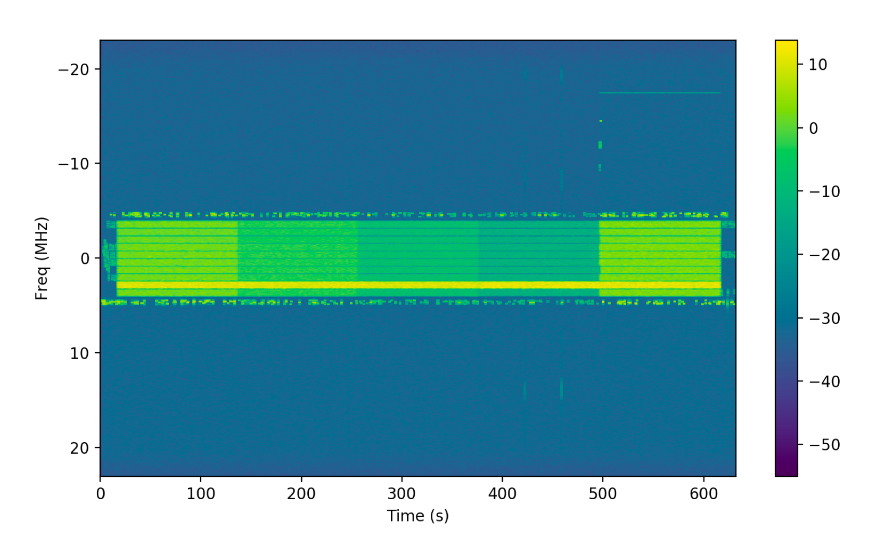
\includegraphics[width = 1.0\textwidth]{Control_Channels_At_Band_Edges.PNG}}
    \caption{The power spectrum observed by an SRN during an SC2 qualification run}
    \label{fig:B.1}
\end{figure}

The second type of control message, i.e., the ``long" control message, contains information regarding traffic statistics, QoS metrics relevant for scoring (SC2 scoring ``rates" the performance of our network as a whole, by assigning points to successfully completed delivery of assigned flows at each source-destination pair in our network), the estimated noise-variance matrix, and DLL flow schedule updates, among others. Each SRN in our network broadcasts these long control messages every second, interleaved with the data traffic\texttt{-{}-}transmitted over the DFT-s-OFDM high data rate link (discussed in \ref{B.I.III}) using the center frequency and bandwidth assigned to this SRN by the Gateway SRNs current channel allocation strategy. Fig. \ref{fig:B.1} illustrates the fact that ``short" control transmissions employ the upper and lower band-edges of the spectrum, while ``long" control transmissions are interleaved with data and sent over the four wideband channels.
\subsection{The DFT-s-OFDM Data Link}\label{B.I.III}
As outlined in Section \ref{B.I.II}, both data traffic and ``long" control message traffic are transmitted by the SRNs in our network over the high data rate Discrete Fourier Transform-spread-Orthogonal Frequency Division Multiplexing (DFT-s-OFDM) channel\texttt{-{}-}using the center frequency and bandwidth assigned to the corresponding SRN, according to the current channel access action determined by the Gateway SRN. Each SRN, upon receiving the current channel and bandwidth allocations for all the other $\tilde{\Lambda}{-}1$ SRNs in our network\texttt{-{}-}over the FSK control link (i.e., ``short" control messages) described in Section \ref{B.I.II}\texttt{-{}-}tunes its $\tilde{\Lambda}{-}1$ receive chains to these $\tilde{\Lambda}{-}1$ channels (center frequency and bandwidth information shared by the other SRNs over the FSK control link), and is therefore able to receive transmissions from all the other SRNs in our network. Additionally, these receive chains perform Schmidl \& Cox time synchronization and frequency offset compensation, in addition to channel noise variance estimation and frequency-domain equalization. All waveforms in this high data rate link constitute $128$ sub-carriers: $108$ are used for data symbols, $12$ are used for pilot symbols, and the remaining $8$ are used for null transmissions that are essential for channel noise variance estimation (the estimates are used in the MCS adaptation technique described in Section \ref{B.I.IV}).
\begin{figure} [htb]
    \centerline{
    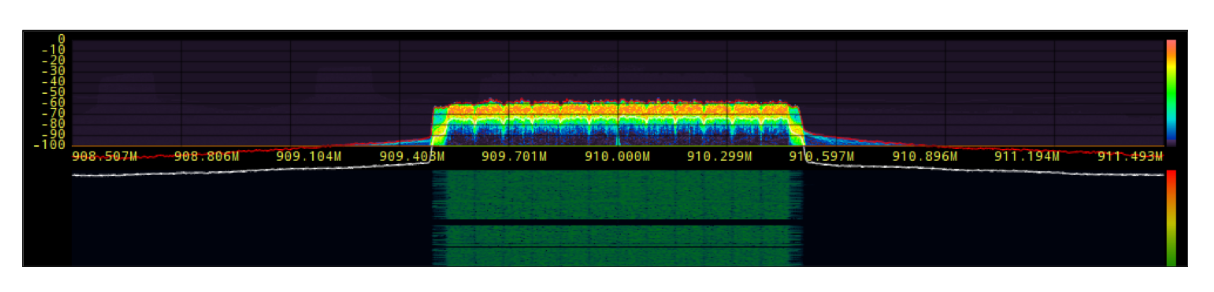
\includegraphics[width = 1.0\textwidth]{Data_Channel_DFT-spread-OFDM_Power_Spectrum.PNG}}
    \caption{The power spectrum of the DFT-s-OFDM waveform}
    \label{fig:B.2}
\end{figure}

A segment, which is the simplest data unit in the Data Link Layer (DLL) of our radio, can an IPv$4$ segment carrying Colosseum data or an IPv$4$ segment carrying ARQ data or a control segment. These segments in the DLL constitute the payload in a frame, which is the simplest data unit in the PHY. A PHY frame consists of a frame header\texttt{-{}-}which contains the source SRN ID, the destination SRN ID, the modulation order and code rate (MCS-$(\mathcal{M},\mathcal{R})$ pair discussed in Section \ref{B.I.IV}) used for the frame payload, a unique identifier for logging, a $32$-bit Cyclic Redundancy Check (CRC), and the number of code-words (blocks) in the frame payload\texttt{-{}-}with the frame header being modulated using QPSK and coded using a rate-$\frac{1}{2}$ Low Density Parity Check (LDPC) code; and the frame payload\texttt{-{}-}which constitutes a sequence of code-words (blocks) populated from a sequence of DLL segments\texttt{-{}-}with this frame payload being modulated and IEEE 802.11 Quasi-Cyclic LDPC (QC-LDPC) coded using an aptly chosen modulation order and code rate (MCS-$(\mathcal{M},\mathcal{R})$ pair discussed in Section \ref{B.I.IV}) which is additionally heralded in the frame header, and finally, mapped onto the sub-carriers of a sequence of OFDM symbols. It is important to note here that, as also discussed in Section \ref{B.I.IV}, the modulation schemes used in our design are QPSK ($\mathcal{M}{=}4$), QAM$16$ ($\mathcal{M}{=}16$), QAM$32$ ($\mathcal{M}{=}32$), and QAM$64$ ($\mathcal{M}{=}64$)\texttt{-{}-}and the code rates ($\mathcal{R}$) used in our design are $\frac{1}{2},\frac{2}{3},\frac{3}{4},\text{ and }\frac{5}{6}$. The power spectrum of the DFT-s-OFDM waveform is illustrated in Fig. \ref{fig:B.2}.
\subsection{Modulation and Coding Scheme (MCS) Adaptation (PHY)}\label{B.I.IV}
The MCS adaptation formulation used in the PHY is a link throughput maximization problem, performed at each individual link $l$ (i.e., a source-destination pair) in our network, subject to constraints on the minimum achieved throughput and maximum allowable bit error probability. This optimization problem involves maximizing the link throughput by finding the modulation order (${=}4,16,32,64$\texttt{-{}-}corresponding to QPSK, QAM$16$, QAM$32$, and QAM$64$, respectively), denoted by $\mathcal{M}$, and the code rate (${=}\frac{1}{2},\frac{2}{3},\frac{3}{4},\frac{5}{6}$), denoted by $\mathcal{R}$, having the smallest Euclidean distance between two circles centered about adjacent symbols in the constellation diagram, with the radius of each of these circles being proportional to the ratio of the estimated standard deviation of the additive channel noise (and the interference from other SRNs on this channel) to the asymptotic code gain. Additionally, in order to remove noise variance measurements with low probabilities of occurrence, we apply a sliding window median filter to the estimated noise variance. Furthermore, as a part of the constraint on the maximum allowable bit error probability, we employ a closed-form approximation for evaluating the bit error probability, denoted by $\mathbb{P}_{b}^{(l)}$, as a function of the noise variance estimate $\hat{\sigma}^{2}$ and the minimum constellation distance $d_{\text{min}}$, given by
\begin{equation}\label{B.4}
    \begin{cases}
        \mathbb{P}_{b}^{(l)}=Q\left(\frac{d_{\text{min}}}{\sqrt{2\hat{\sigma}^{2}}}\right),&\text{ if $\mathcal{M}=4$},\\
        \mathbb{P}_{b}^{(l)}=\frac{4}{\log_{2}(\mathcal{M})}Q\left(\frac{d_{\text{min}}}{\sqrt{2\hat{\sigma}^{2}}}\right),&\text{ if $\mathcal{M}>4$},
    \end{cases}
\end{equation}
where,
\begin{equation}\label{B.5}
    Q(x)=\frac{1}{2\pi}\int_{x}^{\infty}e^{-\frac{y^{2}}{2}}.
\end{equation}
The throughput over this link $l$, denoted by $\rho_{l}$, is given by
\begin{equation}\label{B.6}
    \rho_{l}=\mathcal{R} \cdot BW_{l} \cdot \log_{2}(\mathcal{M}),
\end{equation}
where $BW_{l}$ refers to the bandwidth allocated by the Gateway SRN for this link (based on PSD measurements and collaboration network messages, as a part of the channel access strategy in the MAC).
\begin{figure} [htb]
    \centerline{
    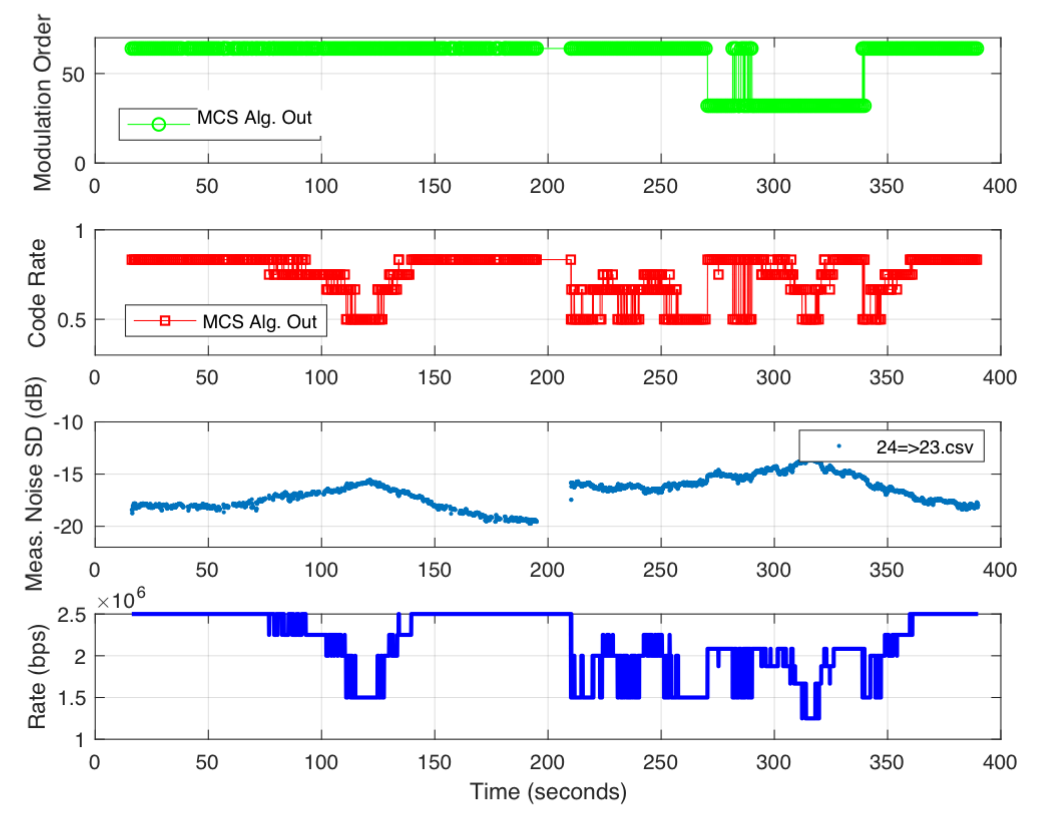
\includegraphics[width = 1.0\textwidth]{Payline_MCS_Adaptation.PNG}}
    \caption{The MCS adaptation scheme during a Payline scenario}
    \label{fig:B.3}
\end{figure}
\begin{figure} [htb]
    \centerline{
    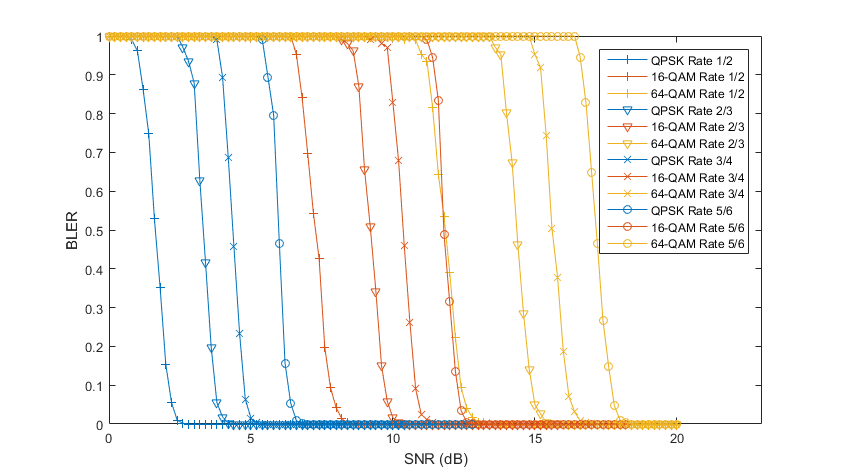
\includegraphics[width = 1.0\textwidth]{BLER.PNG}}
    \caption{The block error rates (BLERs) for different modulation order and code rate pairs, over varying values of SNR (dB)}
    \label{fig:B.4}
\end{figure}

So, at each link (source SRN-destination SRN), upon receiving a NotificationEvent (an inter-module memo in the C${++}$ publish-subscribe software architecture) which indicates a change in the estimated noise variance of the channel used by this link, the MCS adaptation algorithm involves finding the $(\mathcal{M},\mathcal{R})$ pair that has the smallest Euclidean distance between two circles centered about adjacent constellation points, with the radius of each circle given by the ratio of the current estimate of the standard deviation of the channel noise (and the interference caused by other SRNs on this channel) to the asymptotic code gain; subject to minimum required throughput and maximum allowable bit error probability requirements, i.e.,
\begin{equation}\label{B.7}
    \begin{aligned}
        &\min_{\mathcal{M},\mathcal{R}}\ d_{\text{min}}(\mathcal{M},\mathcal{R},\hat{\sigma}),\\
        &\text{subject to}\\
        &\rho_{l} \geq \rho_{l,\text{min}},\text{ and}\\
        &\mathbb{P}_{b}^{(l)} \leq \mathbb{P}_{b}^{(l,\text{max})},
    \end{aligned}
\end{equation}
where $\rho_{l,\text{min}}$ refers to the QoS constraint of supporting a minimum required throughput, $\mathbb{P}_{b}^{(l,\text{max})}$ refers to the maximum allowable bit error probability, $\mathbb{P}_{b}^{(l)}$ is computed using \eqref{B.5}, and $\rho_{l}$ is computed using \eqref{B.6}. Note here that a channel allocation update triggered by the Gateway SRN in our network, induces changes in the estimated (and filtered) noise variance map, which in turn triggers MCS adaptation. Consequently, MCS adaptation triggers an update to the flow schedule in the DLL, which is discussed in Section \ref{B.I.V}. Fig. \ref{fig:B.3} depicts the process of determining the most appropriate modulation order and coding rate adaptive to the changes in the estimated additive channel noise standard deviation. Note here that the link data rate reduces as the channel noise variance increases. Fig \ref{fig:B.4} illustrates the BLock Error Rate (BLER) curves for different combinations of the modulation order and the code rate, over different SNR values.
\subsection{Prioritized Flow Scheduling with ARQ Heuristic (DLL)}\label{B.I.V}
The prioritized flow scheduling algorithm employed in the DLL of our radio involves an adaptive time-quanta based deficit round-robin scheduler with a value-per-resource heuristic and recursive revisitation, in addition to Automatic Repeat reQuest (ARQ) for bursty User Datagram Protocol (UDP) flows (i.e., emulated file transfers). A DARPA SC2 emulation scenario in the Colosseum involves ``mandates" to deliver a variety of flows with pre-specified priorities\texttt{-{}-}quantified by their associated point-values. For instance, Voice Over Internet Protocol (VOIP) traffic is assigned 4 points per flow, the real-time camera feed from an Unmanned Aerial Vehicle (UAV) is assigned 9 points per flow, and the real-time continuous video stream from a water-bomber deployed to fight wildfires in California (emulated scenario) is assigned 15 points per flow. Additionally, a DARPA SC2 scenario also specifically categorizes flows into two groups: intermittent, bursty flows (file transfers) and all other non-bursty traffic.

Based on the available spectrum resources, i.e., channel bandwidth, and the amount of time remaining to complete an assigned flow, each flow is assigned time-quanta\texttt{-{}-}with a non-zero time-quanta assigned to a flow only if it is determined to be likely successful with the given time-quanta. The underlying infrastructure of our scheduler involves individual flow-specific at each SRN in our network\texttt{-{}-}additionally, this includes queues for file bursts and queues for ARQ packets that are supposed to be re-sent to the destination. At each SRN, we employ an ordered resource-fitting heuristic with recursive revisitation wherein we first determine the upper and lower bounds of the resource-block (which termed as a QuantumSchedule)\texttt{-{}-}where the lower bound represents the smallest amount of time required to send a frame corresponding to all the flow-queues at this SRN, subject to the quality of the links; while the upper bound represents the smallest maximum allowable latency among all the flows at this SRN, indicating a temporal resource bound at which ``mandates" start to fail. After determining the upper and lower bounds, based on its assigned flow metrics and quality of its links\texttt{-{}-}each SRN ranks (in decreasing order of priority) its assigned flows according a value-per-resource heuristic, determines the percentage utilization of the QuantumSchedule block for each of these flows (i.e.,  the resource block with the quantified upper and lower bounds), and starts fitting these flows onto the resource block with the added optimization of minimizing the amount of unused resources in this QuantumSchedule block\texttt{-{}-}a recursive revisitation strategy helps the scheduler to recursively perform an ordered fit routine on flows that are yet to be fitted onto the resource block with the intention of completely utilizing the QuantumSchedule block.

In more detail, as and when a new flow is assigned to a particular SRN $i$ in our network, the DLL creates a queue that holds the packets arriving at this SRN from the C2API (discussed in Section \ref{B.II}). When a schedule update is triggered by the arrival of new flows at the SRN, or when the channel and bandwidth allocation changes (as notified by the Gateway SRN via OFDMChannelUpdate NotificationEvents), or when the modulation order and code rate pair changes as a result of the MCS adaptation strategy in the PHY of this SRN (notified internally via MCSRequest NotificationEvents)\texttt{-{}-}the scheduler evaluates the smallest amount of temporal resources needed to serve each flow (on a frame-by-frame basis), i.e.,
\begin{equation}\label{B.8}
    t_{\text{min}}^{(f)}=\frac{f_{\text{ov}}+f_{\text{nseg}}(f_{\text{seg-ov}}+f_{\text{seg-bits}})}{\rho_{l_{f}}},
\end{equation}
where $f_{\text{ov}}$ refers to the frame overhead of flow $f$, $f_{\text{nseg}}$ refers to the number of DLL segments per frame of flow $f$, $f_{\text{seg-ov}}$ denotes a per segment overhead per frame of flow $f$, $f_{\text{seg-bits}}$ is the number of bits per segment of flow $f$, and $\rho_{l_{f}}$ indicates the link throughput\texttt{-{}-}evaluated using the allocated channel bandwidth, the estimated channel noise variance (and interference from competitor SRNs), and the $(\mathcal{M},\mathcal{R})$ pair\texttt{-{}-}with $l_{f}$ referring to the link between the source SRN $i$ and the destination SRN $j$, relevant to this flow $f$. The upper and lower bounds of the QuantumSchedule resource block, for this specific SRN $i$, at this time, are now determined as
\begin{equation}\label{B.9}
    \begin{aligned}
        \text{lb}_{i}&=\sum_{f \in \mathcal{F}_{i}}t_{\text{min}}^{(f)},\text{ and}\\
        \text{ub}_{i}&=\min_{f \in \mathcal{F}_{i}}\delta_{\text{max}}^{(f)},\text{ respectively},
    \end{aligned}
\end{equation}
where $\mathcal{F}_{i}$ refers to the set of all flows assigned to SRN $i$, and $\delta_{\text{max}}^{(f)}$ refers to the maximum allowable latency (QoS constraint) of flow $f$ at SRN $i$. The scheduler then ranks the flows at this SRN according to a value-per-resource metric, i.e., 
\begin{equation}\label{B.10}
    \begin{aligned}
        \text{Rank the flows $f \in \mathcal{F}_{i}$ in the decreasing order of}\\
        \psi_{f}=\frac{V_{f}f_{\text{nseg}}(f_{\text{seg-bits}}-f_{\text{seg-payload-ov}})}{t_{\text{min}}^{(f)}\rho_{l_{f}}},
    \end{aligned}
\end{equation}
where $V_{f}$ denotes the point value of the flow (discussed earlier in this section) $f{\in}\mathcal{F}_{i}$ at SRN $i$, and $f_{\text{seg-payload-ov}}$ denotes the bit overhead in the segment payload per frame corresponding to flow $f$ at SRN $i$. Next, the scheduler ``fits" these flows in a prioritized fashion corresponding to the value-per-resource ranked list of the flows at this SRN, denoted by $\mathcal{S}_{i}$, i.e., flows with a higher value-per-resource metric ($\psi_{f}$) will be fitted first into the QuantumSchedule resource block\texttt{-{}-}if all the flows can be fit into the resource block, we are done; else, the flow with the smallest value-per-resource metric will be removed from this list and added into a revisitation list, denoted by $\tilde{\mathcal{S}}$, and the fitting operation is tried again on the set $\mathcal{S}{-}\tilde{\mathcal{S}}$ in the same prioritized fashion. This procedure takes place until all the flows in the final list $\mathcal{S}$ can be fit into the resource block, with flows (with comparatively lower value-per-resource) which could not be fit into the resource block will be present in $\tilde{\mathcal{S}}$. Next, if there exist no available resources in this QuantumSchedule resource block, the scheduler terminates and publishes the updated schedule to the queueing service controller, thereby leading to all the ``high value-per-resource" flows (present in $\mathcal{S}$) being perfectly scheduled in the available resource block (governed by link quality, allocated bandwidth, and flow-specific QoS constraints). On the other hand, if available resources exist in the QuantumSchedule resource block, the list $\tilde{\mathcal{S}}$ is recursively traversed, again in the decreasing order of the flow value-per-resource heuristic, and each of these value-per-resource ranked ``recursively re-visited" flows are evaluated for their fit into the available/remaining portion of the resource block. These combination of heuristics account for a prioritized flow scheduling strategy in the DLLs of our SRNs\texttt{-{}-}triggered by assigned traffic changes, QoS mandate changes, channel and bandwidth changes, and MCS choice updates; constituting a recursive-revisitation strategy to account for the maximum utilization of an elementary resource block, and a value-per-resource ranking and traversing heuristic to account for the need to prioritize flows that give our network a higher utility per unit resource consumed.

Additionally, ARQ is employed for file flows to ensure that the packets corresponding to these simulated file transfers are reliably sent across the network from the source SRN to the destination SRN. These simulated file transfers correspond to bursty UDP flows, and the packets within these bursts are sequenced by the DLL at the sender SRN. The receiver SRN provides positive acknowledgements (ACKs) for the sequence numbers within a burst which have been successfully received and decoded. A separate ARQ queue is employed in the deficit round-robin queueing infrastructure discussed earlier\texttt{-{}-}based on the feedback from the ARQ mechanism, the scheduler (prioritized value-per-resource strategy with recursive revisitation) dynamically reschedules these ARQ packets for re-transmission\texttt{-{}-}the priority of these ARQ flows deteriorates with every re-transmission.
\subsection{Channel and Bandwidth Allocation Heuristic (MAC)}\label{B.I.VI}
Based on the given initial network conditions (by the Command and Control radio API (C2API) discussed in Section \ref{B.II}), the information gleaned during network discovery over the FSK control channel, and the offered traffic statistics reported by the SRNs over the high data rate DFT-s-OFDM link, the channel and bandwidth allocation algorithm in the Gateway SRN (fusion/data aggregation center) coordinates a center frequency and bandwidth assignment to all the back-logged SRNs in our network. An environment update\texttt{-{}-}such as a change to the offered traffic at certain SRNs, or a change in the minimum required throughput and maximum allowable latency QoS constraints for certain traffic flows, or a change in the overall available RF spectrum bandwidth in the scenario, among others; or a performance notification from our peers, or incumbents (see Section \ref{B.I.I}), or our network coordinator (i.e., self: the Gateway SRN)\texttt{-{}-}indicating that the ensemble is performing poorly due to the over-exploitation of spectrum resources by our network, or that the ensemble transmissions are interfering with the incumbent resulting in the aggregate interference observed at the incumbent being higher than the current threshold, or that our network is failing to satisfy the QoS requirements for a significant number of traffic flows for the past pre-specified duration of time (typically, 10 seconds), respectively\texttt{-{}-}triggers a change in the channel and bandwidth allocation.

We decompose this problem into two sub-problems: bandwidth allocation and subsequent center-frequency assignment. Based on the emulation scenario bandwidth, the Gateway SRN's bandwidth allocation strategy assigns bandwidths to each SRN in the network based on the amount of traffic offered to the SRN, the QoS requirements imposed on each of these traffic flows, and the quality of the links.
\begin{figure} [htb]
    \centerline{
    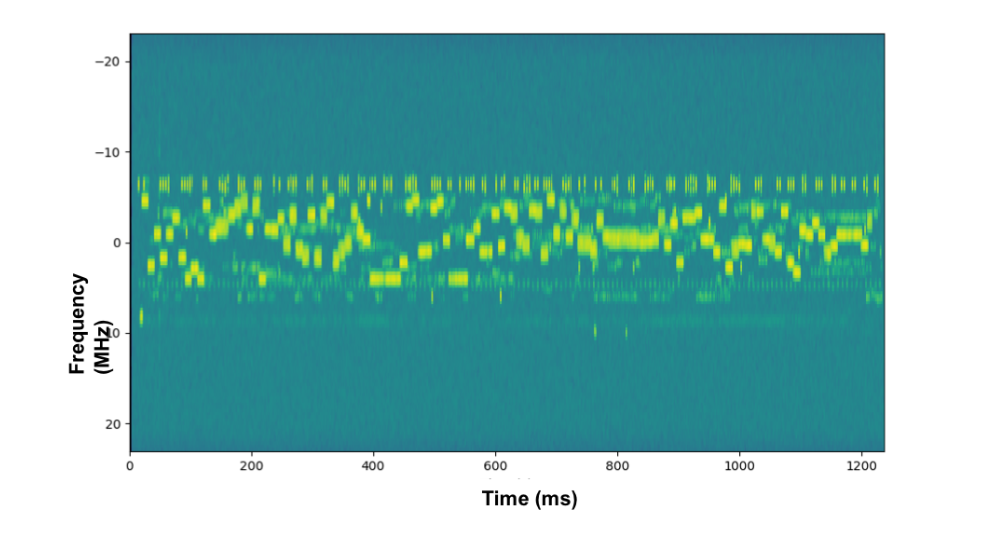
\includegraphics[width = 1.0\textwidth]{Alleys_of_Austin_Channel_Access.PNG}}
    \caption{The spectrum occupied by our network during an Alleys of Austin scenario emulation}
    \label{fig:B.5}
\end{figure}

Post-bandwidth assignment, the channel allocation sub-problem is taken up by the Gateway SRN: it should determine the center frequencies that minimize interference from (and in turn interference to) the other competitors' SRNs in the emulation scenario, while achieving the mandated minimum required throughput and maximum allowable latency QoS constraints imposed on each traffic flow (additional QoS constraints can be imposed on file transfer flows\texttt{-{}-}typically, the time window within which the file transfer needs to be completed from the source SRN to the destination SRN within our network). In order to obtain a complete picture about the spectrum occupancy at a specific SRN in our network (i.e., at a particular location), we exploit two kinds of data: CIL messages from the other competitor networks in the emulation scenario\texttt{-{}-}specifically, the SpectrumUsage messages and the LocationUpdate messages; and the PSD measurements made at the SRN. The Gateway SRN's channel allocation heuristic employs the data gleaned from the SpectrumUsage and LocationUpdate CIL messages broadcasted over the collaboration network by the other competitors in the emulation scenario, and the collated location-specific PSD measurements in the following fashion: first, the channel gain between a pair of SRNs in our network is estimated based on their location information (which is typically obtained from the C2API, if not, it is obtained from the periodic GPS NotificationEvents published by individual SRNs and sent to the Gateway SRN over the high data rate DFT-s-OFDM control link (interleaved with data)) and an empirical path loss exponent; second, based on this estimated channel gain\texttt{-{}-}and a weighted combination of collated PSD measurements and competitor CIL messages\texttt{-{}-}the Gateway SRN determines the amount of interference experienced by our SRNs in each of these channels, and performs a heuristic search to determine the center frequencies that minimize the total interference caused at our SRNs. Fig.\ref{fig:B.5} illustrates the spectrum occupancy of SRNs in our network (as seen by one SRN\texttt{-{}-}collated using PSD measurements and internal occupancy notifications from the Gateway SRN).
\subsection{Multi-hop Routing Heuristic (NET)}\label{B.I.VII}
When the ``short" control messages over the FSK control channel cannot be received by SRN $i$ from SRN $j$ for a pre-determined amount of time (typically, $10$ seconds), the link $l_{ji}$ is reported to be blocked/down by SRN $i$ (similar behavior by all the other SRNs in our network). This routinely occurs in any given DARPA SC2 emulation scenario due to the presence of emulated physical obstacles (hills, buildings, etc.), or the presence of jammers in the network, or the emulation of node mobility characteristics, or high noise and interference in the spectrum as a whole resulting in failed decoding of the short control message packets sent over the FSK control channel (which uses the band-edges of the spectrum). On the other hand, a successful/working link is reported by SRN $i$ with respect to link $l_{ji}$, if short control message packets from SRN $j$ can be successfully decoded. Hence, a binary vector can be constructed at each individual SRN indicating the status of its incoming links\texttt{-{}-}which is then shared with all the other SRNs in the network over the FSK control channel, in order to build a routing table at each SRN, which is periodically updated throughout the emulation.

During data transmission, assuming a correct and current routing table exists at each SRN (which is true because of the periodic updates sent from all the other SRNs over the robust FSK control link), in the Network layer (NET) of each SRN, Dijkstra's algorithm is applied to this routing table, to find the route to the destination SRN using the smallest number of hops.
\section{The Colosseum Command and Control radio API (C2API)}\label{B.II}
The Colosseum Command and Control API (C2API), also referred to as the Radio C2API, is an interface of four shell scripts\texttt{-{}-}namely, start.sh, stop.sh, status.sh, and statistics.sh; which should be supported by every SRN in the deployment, and the combinations of which are used by the scenario emulator, i.e., the Colosseum, in any given deployment, to orchestrate the following activities \cite{DARPA:SC2c2api}:
\begin{itemize}
    \item Notify all the SRNs in the deployment of changes to the radio environment, i.e., changes to the available scenario bandwidth, Passive Incumbent center frequency and threshold changes (discussed in Section \ref{B.I.I}), and scenario stage resets;
    \item Notify all the SRNs in the deployment of their respective newly assigned traffic flows and the QoS constraints (termed ``Individual Mandates (IMs)") for each of them\texttt{-{}-}in addition to performance mandates for a competitor network as a whole (termed ``Network Mandated Outcomes");
    \item Provide static Colosseum configuration information such as the channel emulator's operating frequency, in addition to collaboration network parameters; and
    \item Administration and Management of individual SRNs in individual competitor networks in the deployment, throughout the scenario execution process.
\end{itemize}
\section{The CIRN Interface Language (CIL)}\label{B.III}
As discussed earlier, the DARPA SC2 Grand Challenge involves a collaboration channel (outside the RF environment) that facilitates the cooperative exchange of crucial operational and performance messages among competing CIRNs\texttt{-{}-}in order to not only ensure optimal performance by individual competitor networks, but also by the ensemble, as a whole. By design, every competitor network should have a designated gateway node that communicates with other competitors in the deployment, over the collaboration channel. The gateway SRN corresponding to every competitor network in the deployment will connect to a collaboration server over a wired IP link (ip\_addr:access\_interface), with this collaboration server acting as a publisher-subscriber\texttt{-{}-}tracking competitor SRNs in the deployment, and re-directing peer-to-peer collaboration traffic from the sender gateway to the destination gateway \cite{DARPA:SC2collaboration}.

The collaboration API involves two types of messages \cite{DARPA:SC2collaborationprotocol}:
\begin{itemize}
    \item Client-Server: a set of procedures and semantics to be followed by competitor networks in the deployment, while interacting with the collaboration server in order to ``discover" the addresses of other competitors in the scenario emulation; and
    \item Peer-to-Peer: a set of procedures and semantics that forms the crux of the CIRN Interface Language (CIL) specifications, and is used to describe the collaborative information exchange between two competitor networks in the deployment.
\end{itemize}
The format/structure/semantics of these messages are described in the now standardised CIL protocol specifications. We list a few important collaboration client-server and peer-to-peer messages below:
\begin{itemize}
    \item TalkToServerMessage: All client-server messages, i.e., the messages from a gateway SRN to the collaboration server, should be formatted according to this top-level wrapper\texttt{-{}-}derived instances include Register (a gateway SRN wishes to register its network with the collaboration server), KeepAlive (serves as a heartbeat message from the gateway, informing the collaboration server that it is still active), and Leave (a gateway SRN informs the collaboration server that its network wishes to leave the collaboration channel);
    \item TalkToClientMessage: All messages from the collaboration server to the client are instances of this parent structure\texttt{-{}-}encapsulates Inform (response to Register from the client: the collaboration server sends the unique client ID, maximum keep-alive count, and a list of registered competitors in the collaboration network (i.e., their client IDs and IP addresses); and Notify (the collaboration server broadcasts to all registered clients on the collaboration network that either a new competitor has successfully registered with it, or an existing competitor has left the collaboration channel);
    \item CilMessage: A top-level wrapper encapsulating all peer-to-peer messages in the collaboration network\texttt{-{}-}specifically, IncumbentNotify and IncumbentPassiveInfo (Passive Incumbent messages: discussed in Section \ref{B.I}), LocationUpdate (GPS location information for all SRNs in a competitor network), SpectrumUsage (the exact spectrum voxels, i.e., time-frequency resources, being accessed by SRNs in a competitor network, along with their perceived importance to satisfying the network's assigned mandates), and DetailedPerformance (total number of QoS constraints assigned, total number of QoS constraints satisfied, total score achieved, score threshold for ensemble utility optimization, etc.).
\end{itemize}
\section{Capabilities and Performance Evaluations from DARPA SC2 scenario emulations}\label{B.IV}
In this section, we present plots illustrating the operational capabilities and the performance of our SRNs (and our network, as a whole) in a military deployment scenario, i.e., Alleys of Austin, and a disaster relief deployment scenario, i.e., Wildfire.
\subsection{Alleys of Austin}
This emulated military deployment scenario in the Colosseum, involves a $45$-member platoon (with an Unmanned Aerial Vehicle (UAV)) from the Texas Army National Guard practicing urban maneuvers and communications in Austin, Texas. The platoon is divided into $5$ squads, with $9$ members in each squad, and is moving through the streets of Austin in three stages\texttt{-{}-}involved in basic voice communications in Stage $1$, Stage $2$ involves the exchange of voice, imagery, and video, and Stage $3$ involves a significant increase in the amount of traffic (voice, imagery, and video) exchanged among the squad members. Each competitor CIRN represents a squad\texttt{-{}-}thereby resulting in a $5$ team, $50$ node ($5{\cdot}9{=}45$ SRNs${+}5{\cdot}1{=}5$ gateway SRNs, with an emulated UAV), large-scale, small packet, military deployment scenario, employing a single-tap propagation model \cite{DARPA:SC2scenarios}. Each team must achieve $50$\% of the QoS mandates assigned to it, during the scenario emulation\texttt{-{}-}in a given time snapshot, teams get scores only if every competitor network achieves their corresponding desired performance in that time snapshot, thereby each competitor is incentivized to work with the others in the network in achieving the required mandates.
\begin{figure} [htb]
    \centerline{
    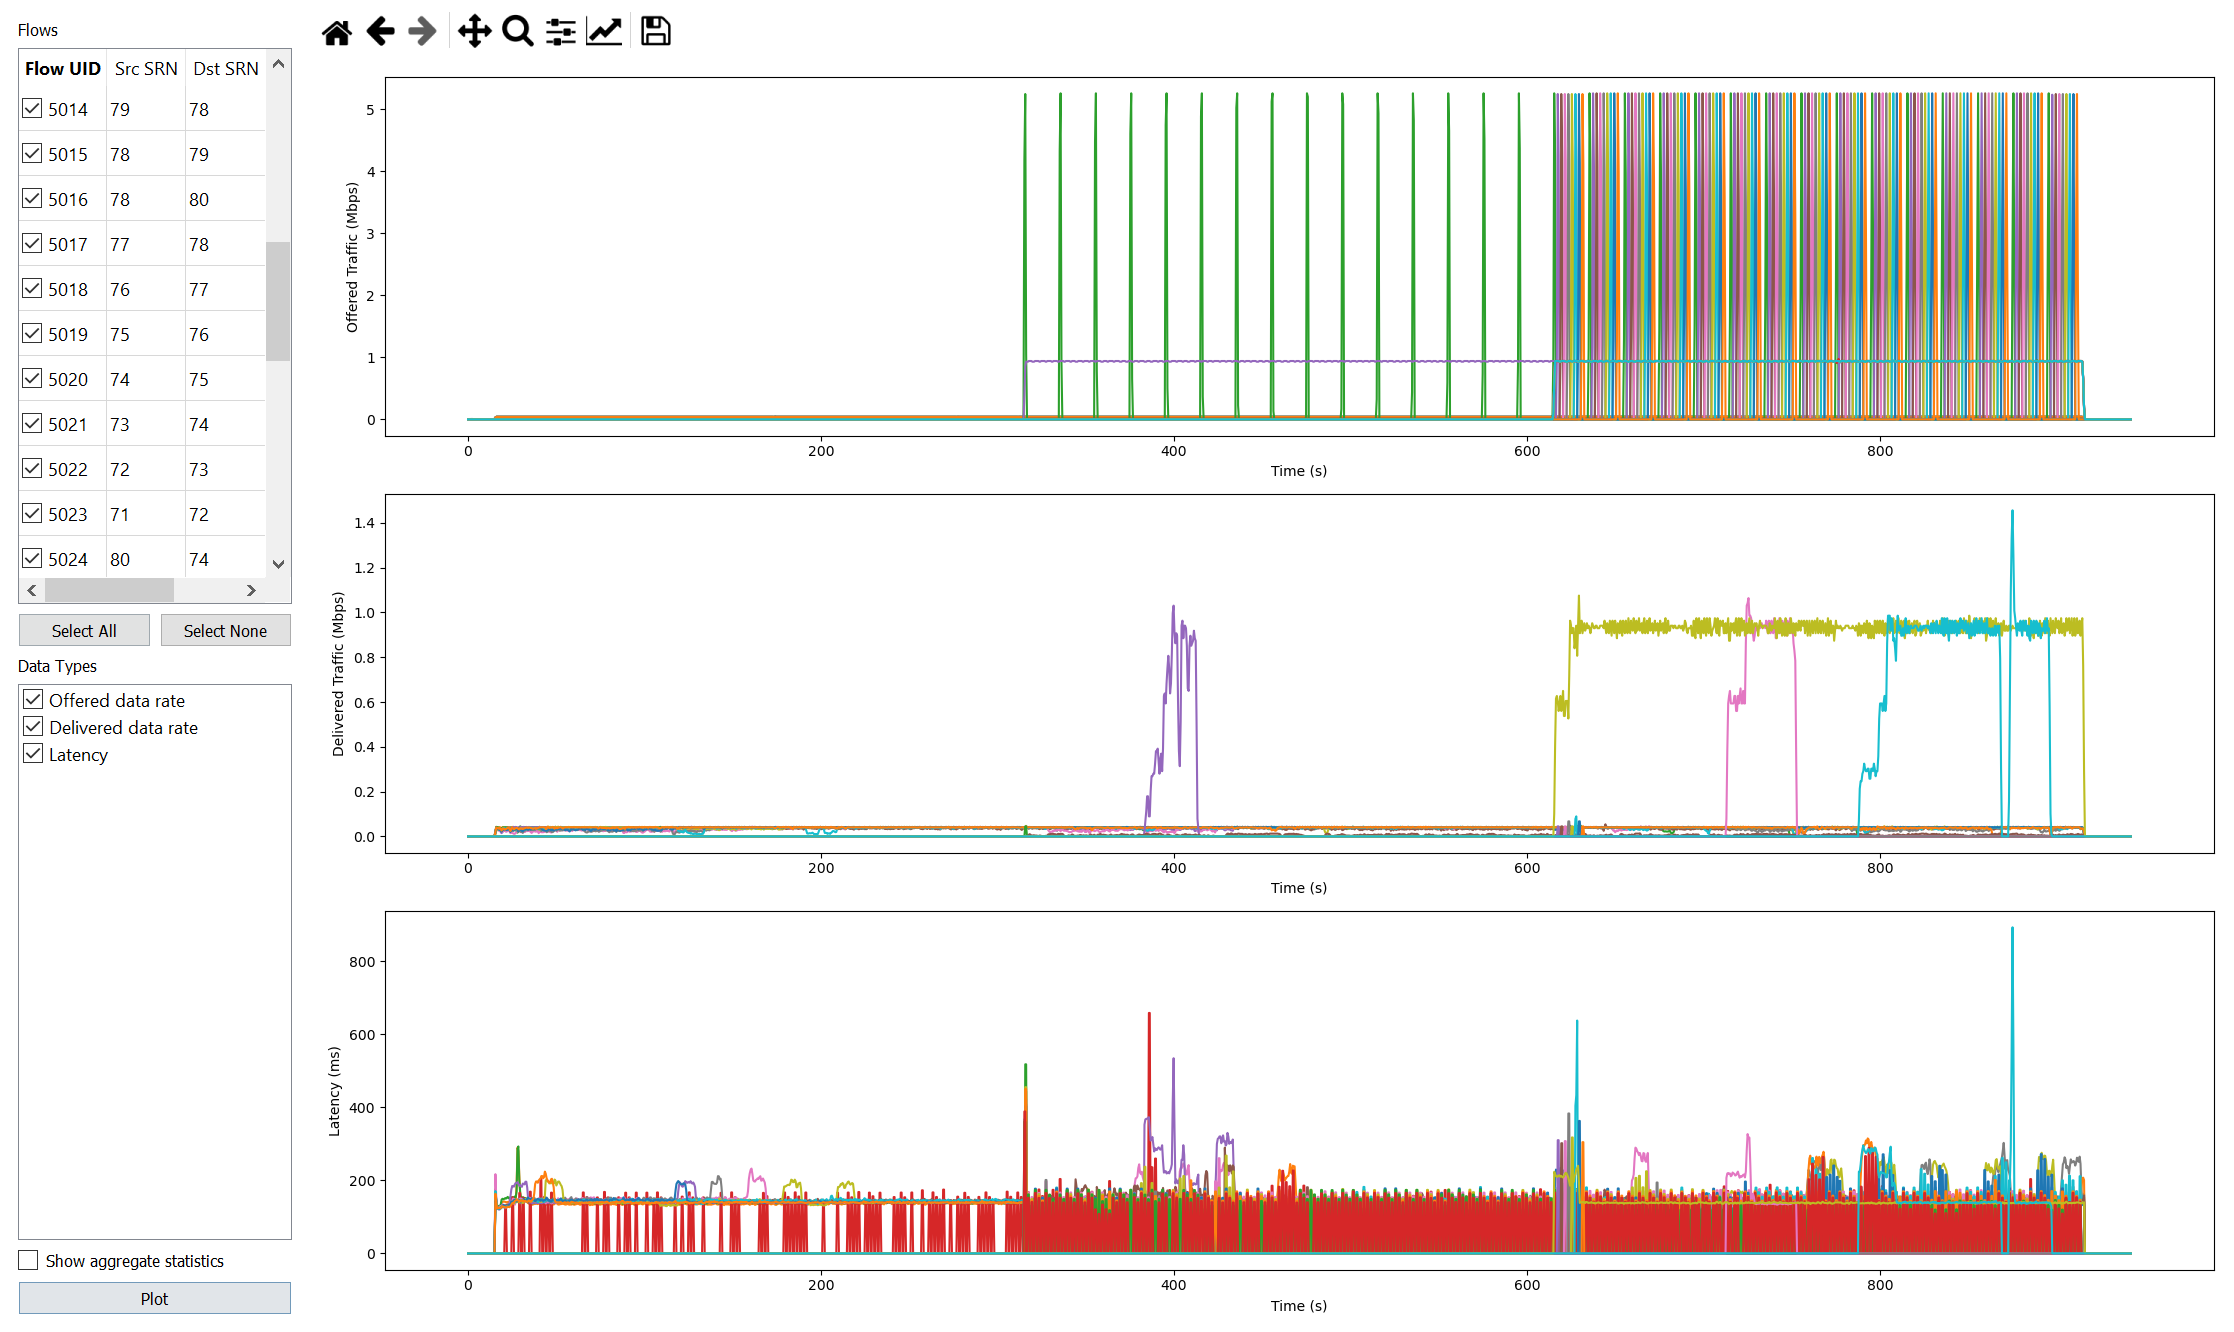
\includegraphics[width = 1.0\textwidth]{Alleys_NET.PNG}}
    \caption{The offered and delivered traffic corresponding to various (selected) flows during the Alleys of Austin scenario emulation}
    \label{fig:B.6}
\end{figure}

Fig. \ref{fig:B.6} illustrates the offered traffic corresponding to the individual selected flows, their corresponding delivered traffic, and the latency experienced by these flows as they are being scheduled/delivered by our network. Note here that our network is able to deliver almost all of these flows with minimal latency. Also, note the stages in the scenario emulation\texttt{-{}-}as described earlier, Stage $1$ constitutes basic voice traffic, i.e., the initial flows have a low offered traffic data rate of $40$kbps; Stage 2 constitutes voice, imagery, and video traffic, i.e., the flows in this Stage have low offered traffic data rate, but imagery and video flows carry higher point values (flow priorities); and finally Stage $3$ involves a significant increase in the amount of offered traffic for the voice, imagery, and video flows. From Fig. \ref{fig:B.6}, we observe that our network is able to deliver most of the flows in Stages $1$ and $2$\texttt{-{}-}however, in Stage $3$, as is usually expected, due to the extremely high offered traffic, our network is not able to satisfy all the assigned flows.
\begin{figure} [htb]
    \centerline{
    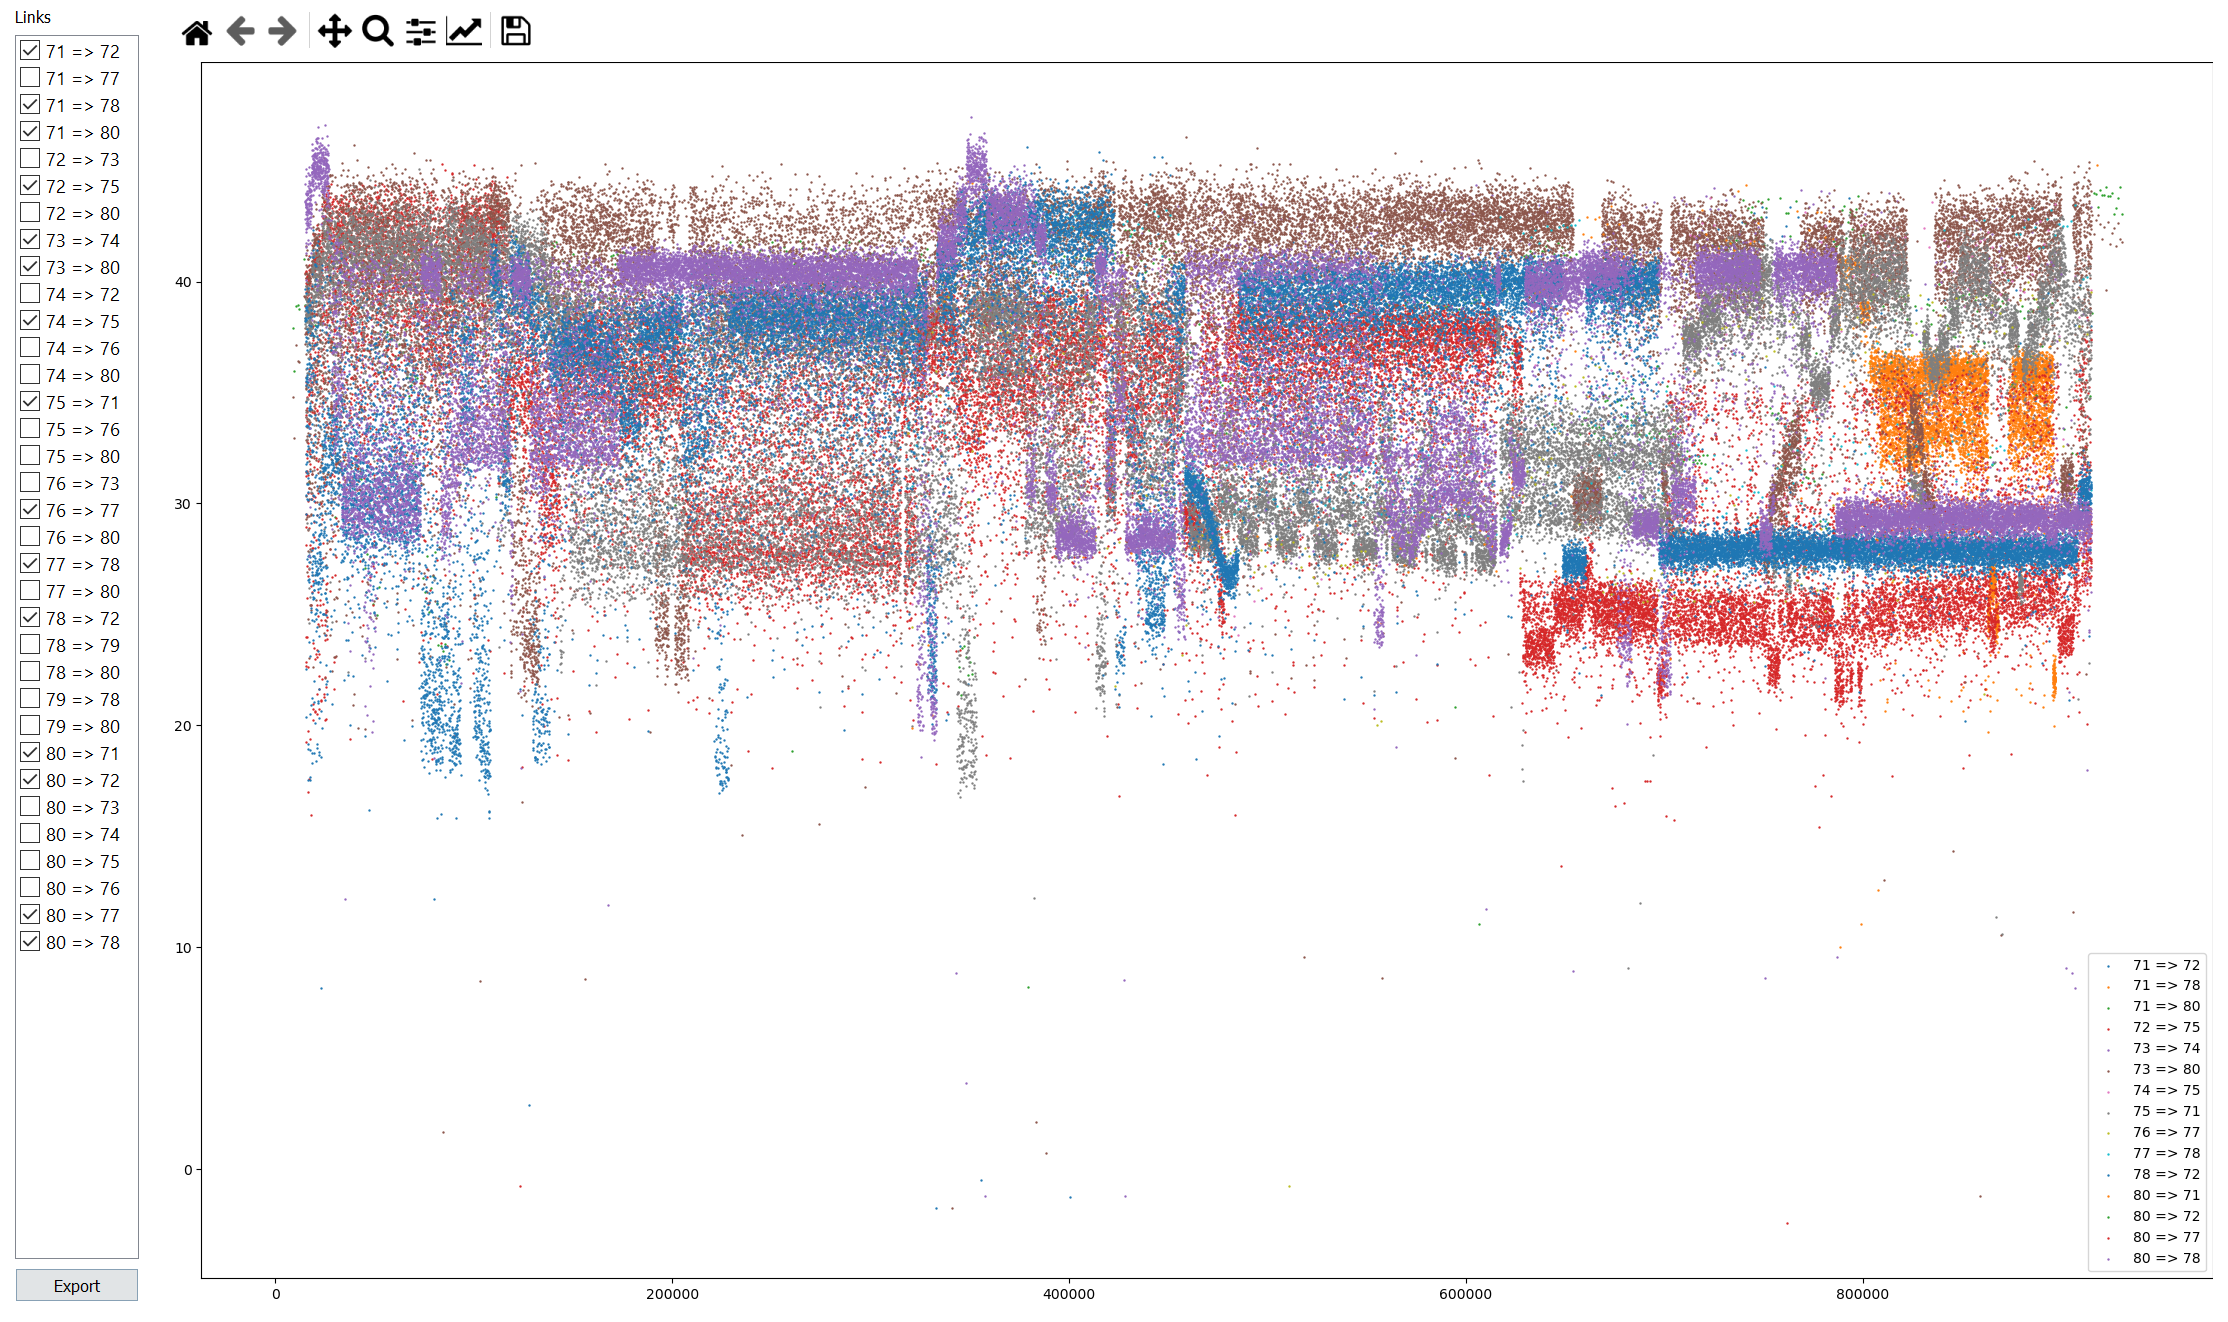
\includegraphics[width = 1.0\textwidth]{Alleys_SNR.PNG}}
    \caption{The estimated SNR on various (selected links) during the Alleys of Austin scenario emulation}
    \label{fig:B.7}
\end{figure}
\begin{figure} [htb]
    \centerline{
    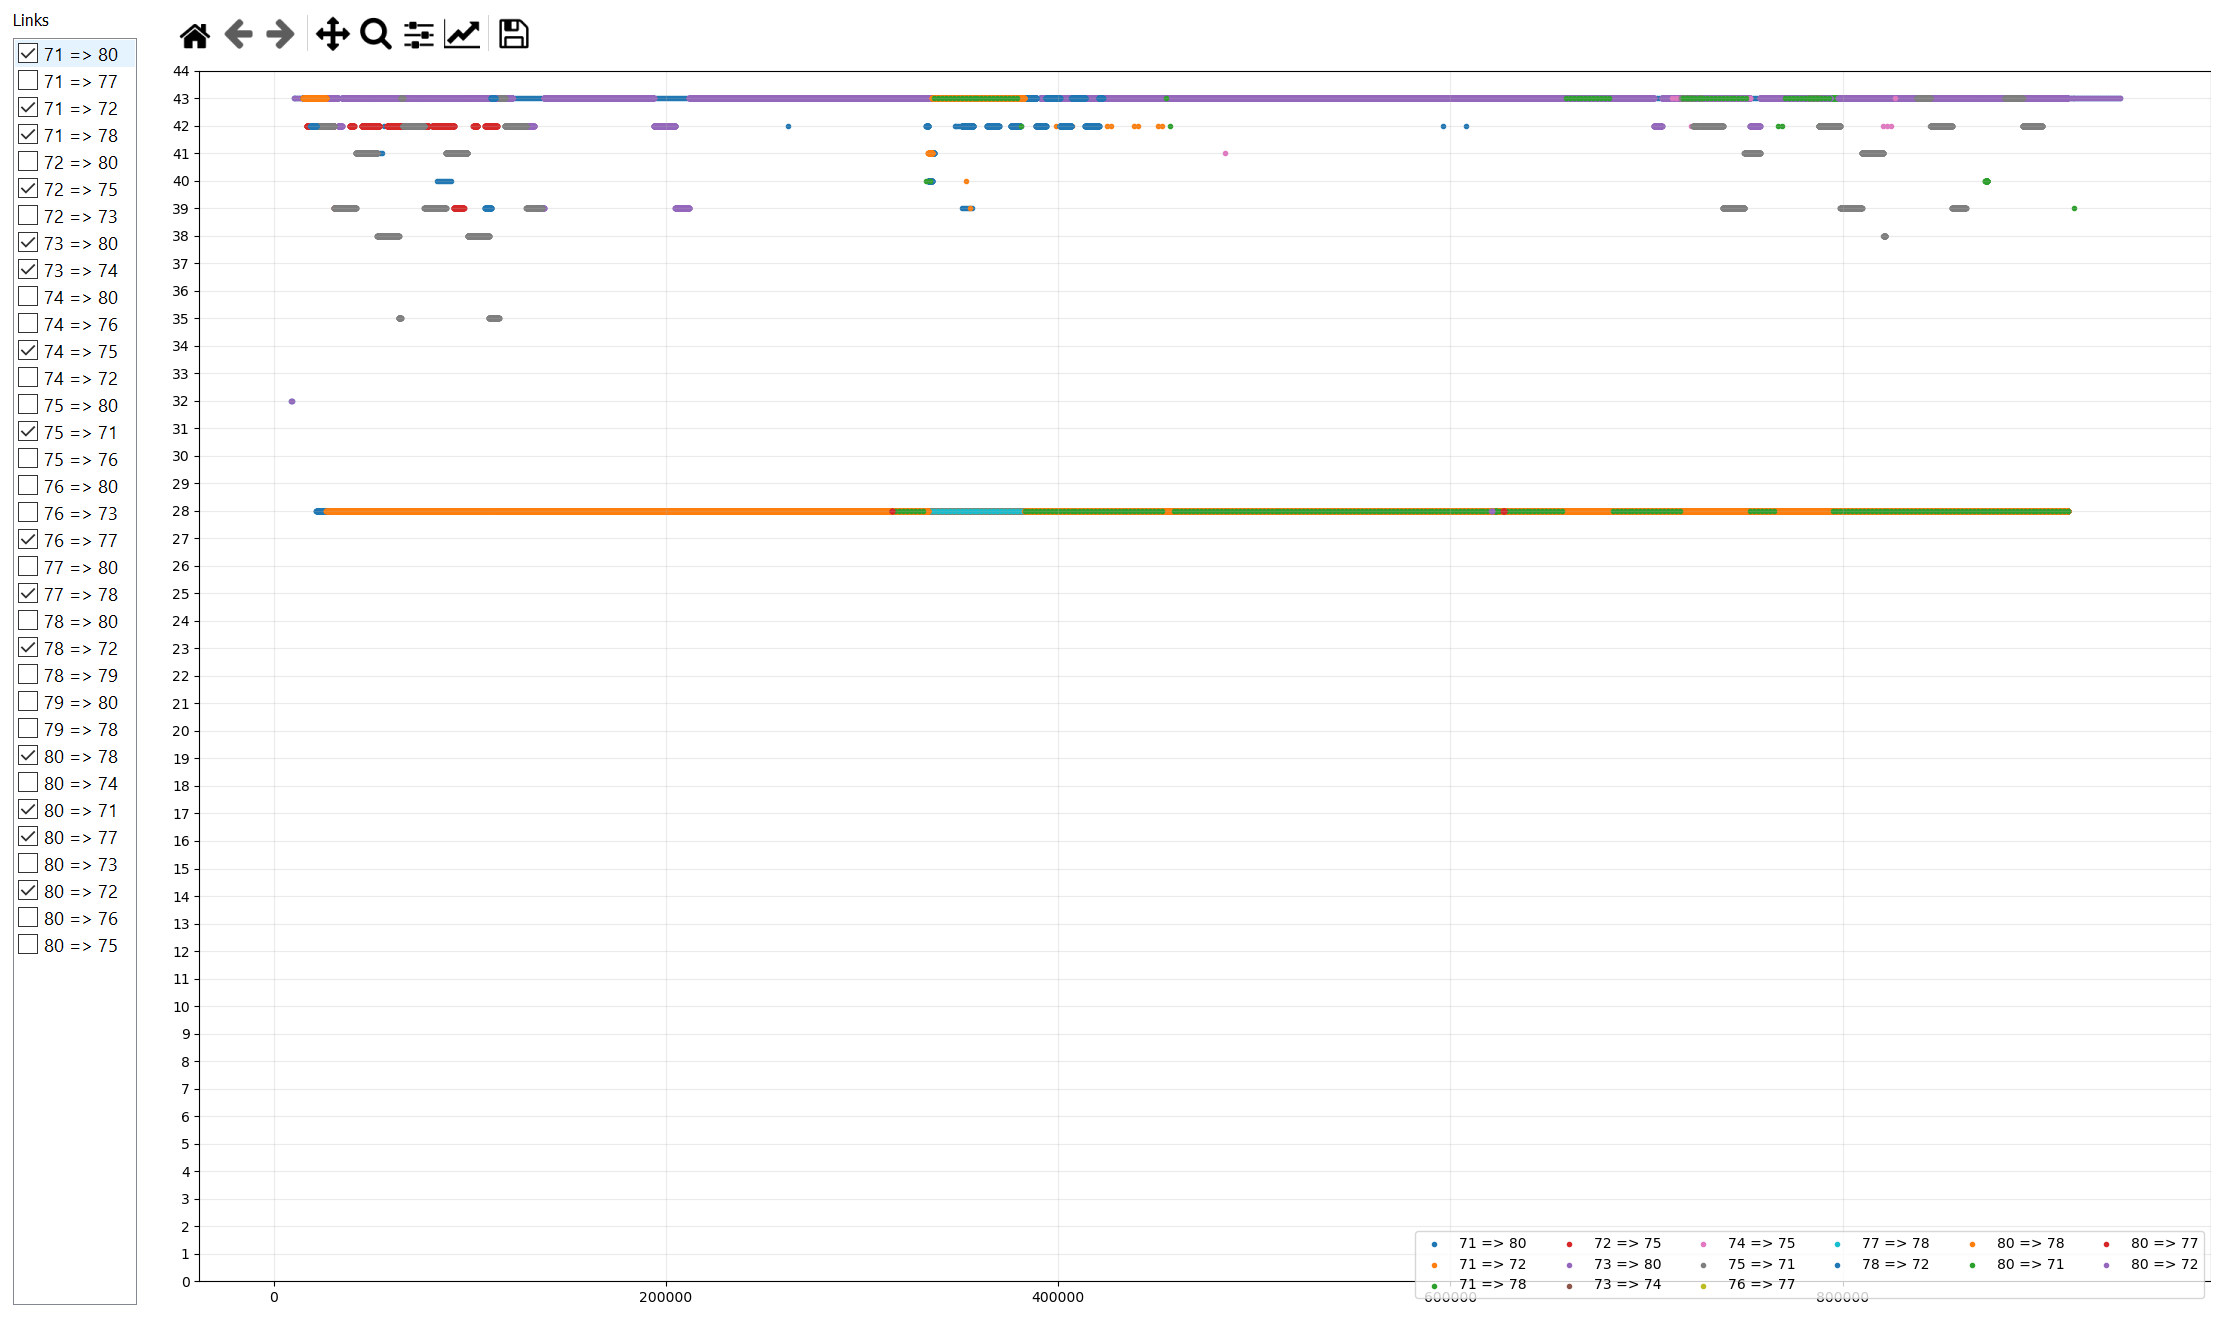
\includegraphics[width = 1.0\textwidth]{Alleys_MCS.PNG}}
    \caption{The MCS adaptation scheme at each (selected) link during the Alleys of Austin scenario emulation}
    \label{fig:B.8}
\end{figure}

Fig. \ref{fig:B.7} depicts the estimated SNR on various selected links (source SRN - destination SRN), during the progression of the Alleys of Austin scenario\texttt{-{}-}these SNR estimates at each link are, as discussed earlier, employed in the MCS adaptation scheme, the prioritized flow scheduler, and the bandwidth allocation algorithm. Consequently, Fig. \ref{fig:B.8} depicts the MCS adaptation scheme at each of these selected links, adapting to the changing estimated SNR with respect to the corresponding channels used by these links\texttt{-{}-}the Y-axis of the MCS adaptation plot in Fig. \ref{fig:B.8} refers to the C${++}$ enumeration value corresponding to the $(\mathcal{M},\mathcal{R})$ pair, i.e., for example, $43$ in the plot refers to QAM$64$ modulation with a code rate of $\frac{5}{6}$, while $28$ refers to QPSK modulation with $\frac{1}{2}$ code rate\texttt{-{}-}in other words, the highest modulation order used in this Alleys of Austin run is $\mathcal{M}{=}64$ (i.e., QAM$64$), while the lowest modulation order used in $\mathcal{M}{=}4$ (i.e., QPSK).
\begin{figure} [htb]
    \centerline{
    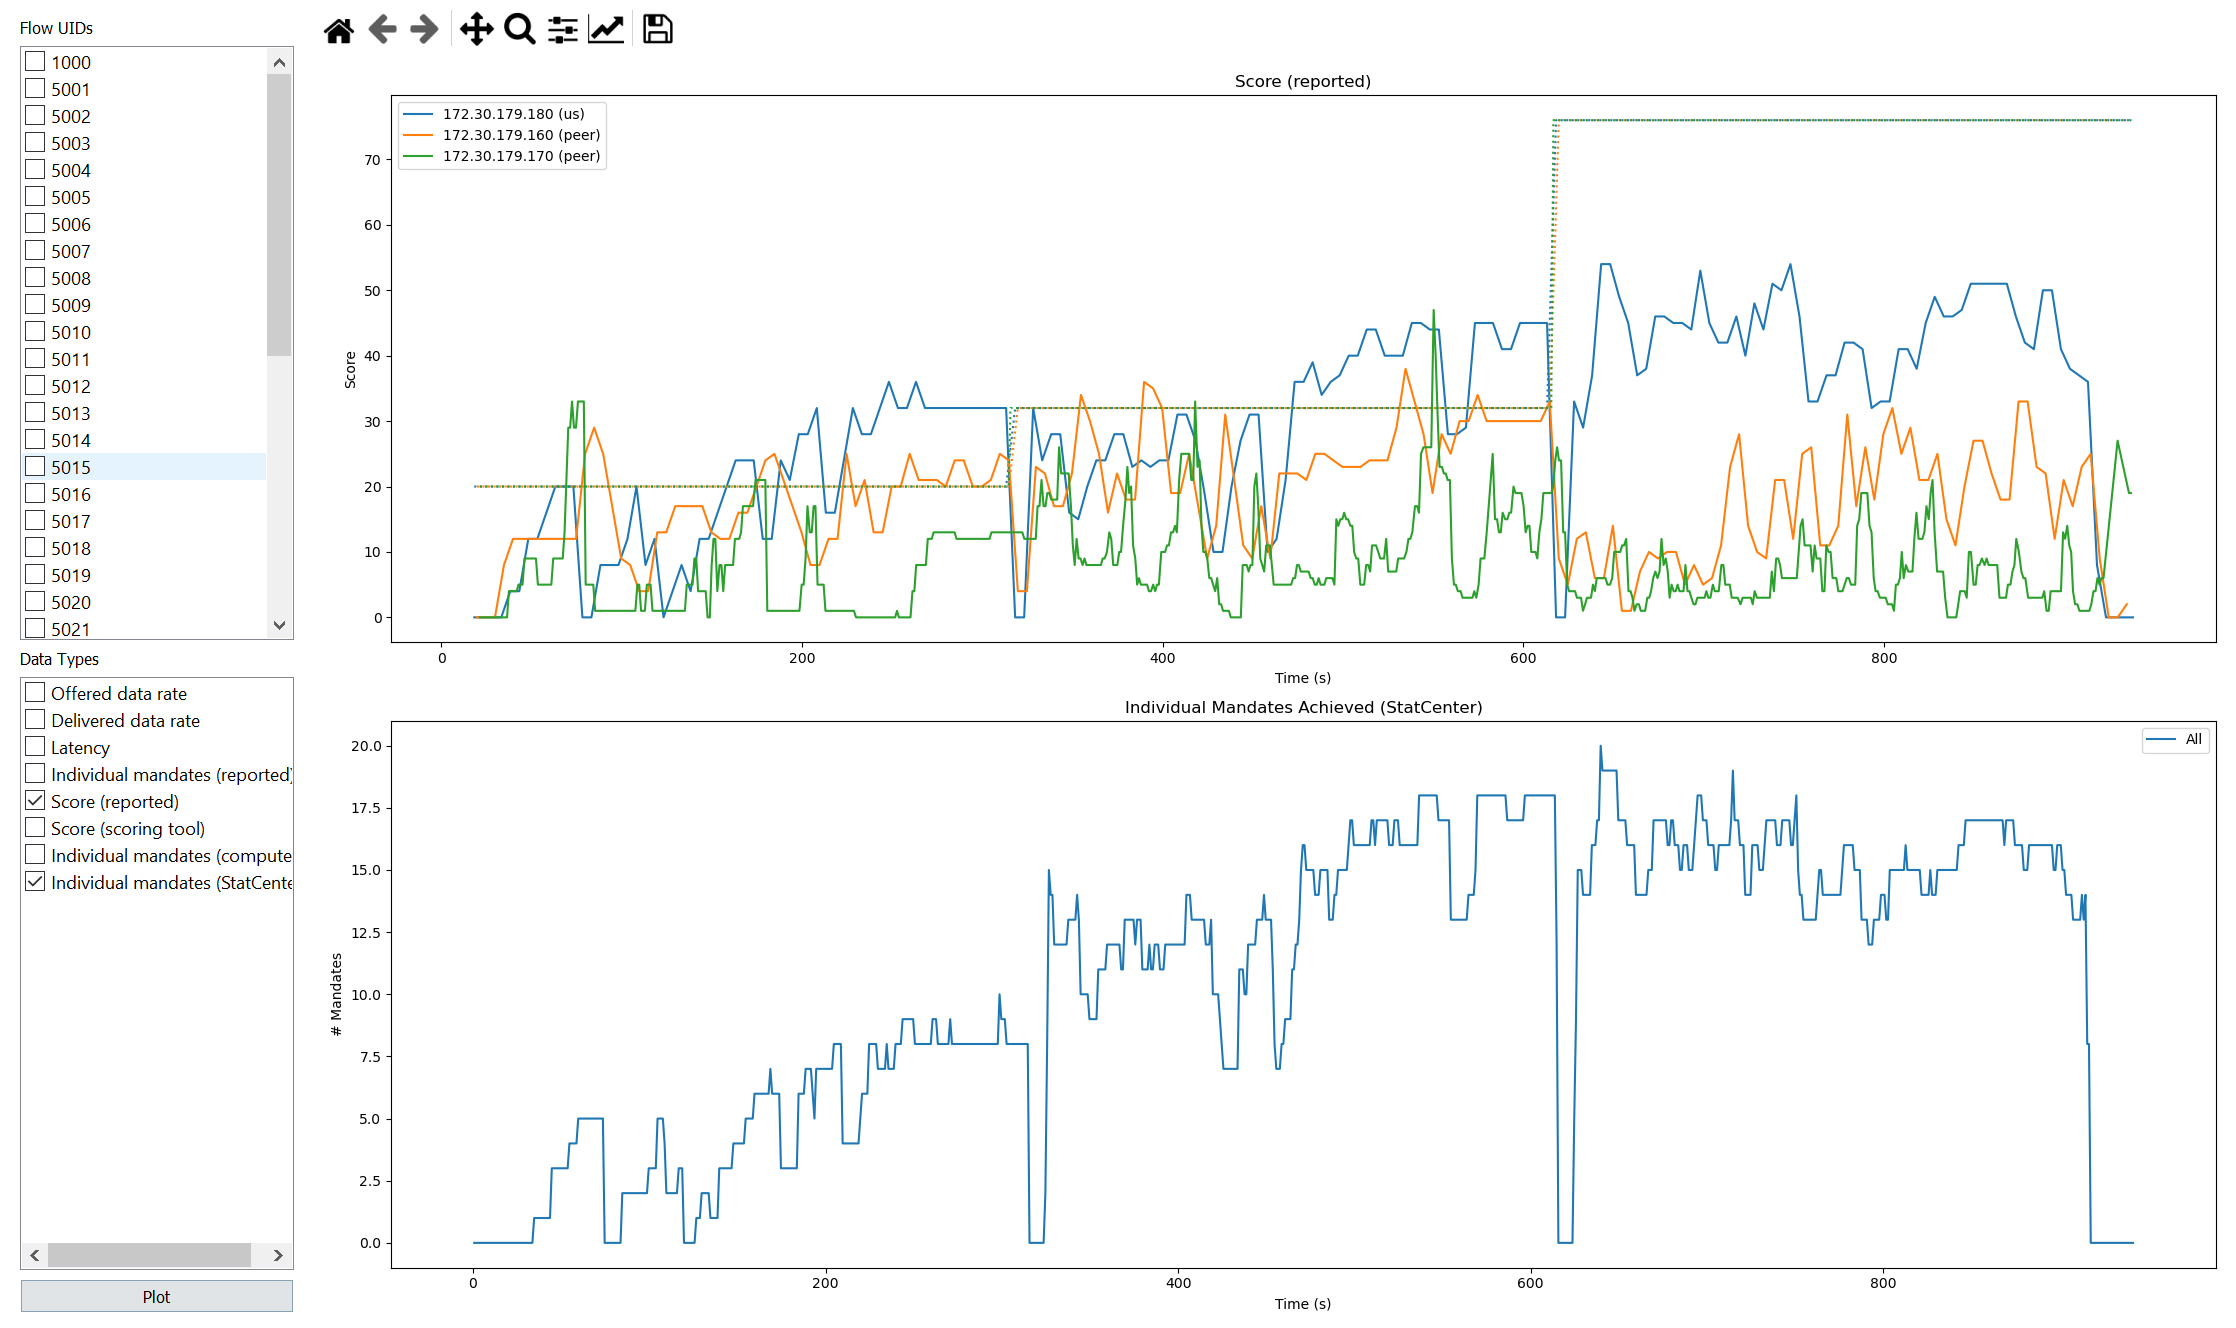
\includegraphics[width = 1.0\textwidth]{Alleys_Scoring.PNG}}
    \caption{The scores attained by our network and other competing networks during the Alleys of Austin scenario emulation, in addition to the number of QoS mandates satisfied by our network in a given time snapshot}
    \label{fig:B.9}
\end{figure}

Fig. \ref{fig:B.9} illustrates the score obtained by our network (indicated by our Gateway SRN's IP address) along with the scores obtained by our peers (indicated by the IP addresses of their corresponding gateway SRNs) in the scenario emulation. The dotted lines in the first sub-plot indicate the score thresholds that need to be achieved by each network, in a Stage. As is evident from the figure, our network satisfies/exceeds the score threshold in Stages $1$ and $2$, but fails in Stage $3$\texttt{-{}-}however, our network does have the best performance among all the teams in the scenario emulation. It is important to note here that even though there were $5$ teams in the emulation of this Alleys of Austin scenario, only the scores of $3$ of them are visualized in this figure\texttt{-{}-}$2$ teams did not report their scores over the collaboration network, and hence their scores were not visualized in this illustration. The second sub-plot illustrates the number of flow-specific QoS mandates that were achieved by our network in a given time snapshot.
\begin{figure} [htb]
    \centerline{
    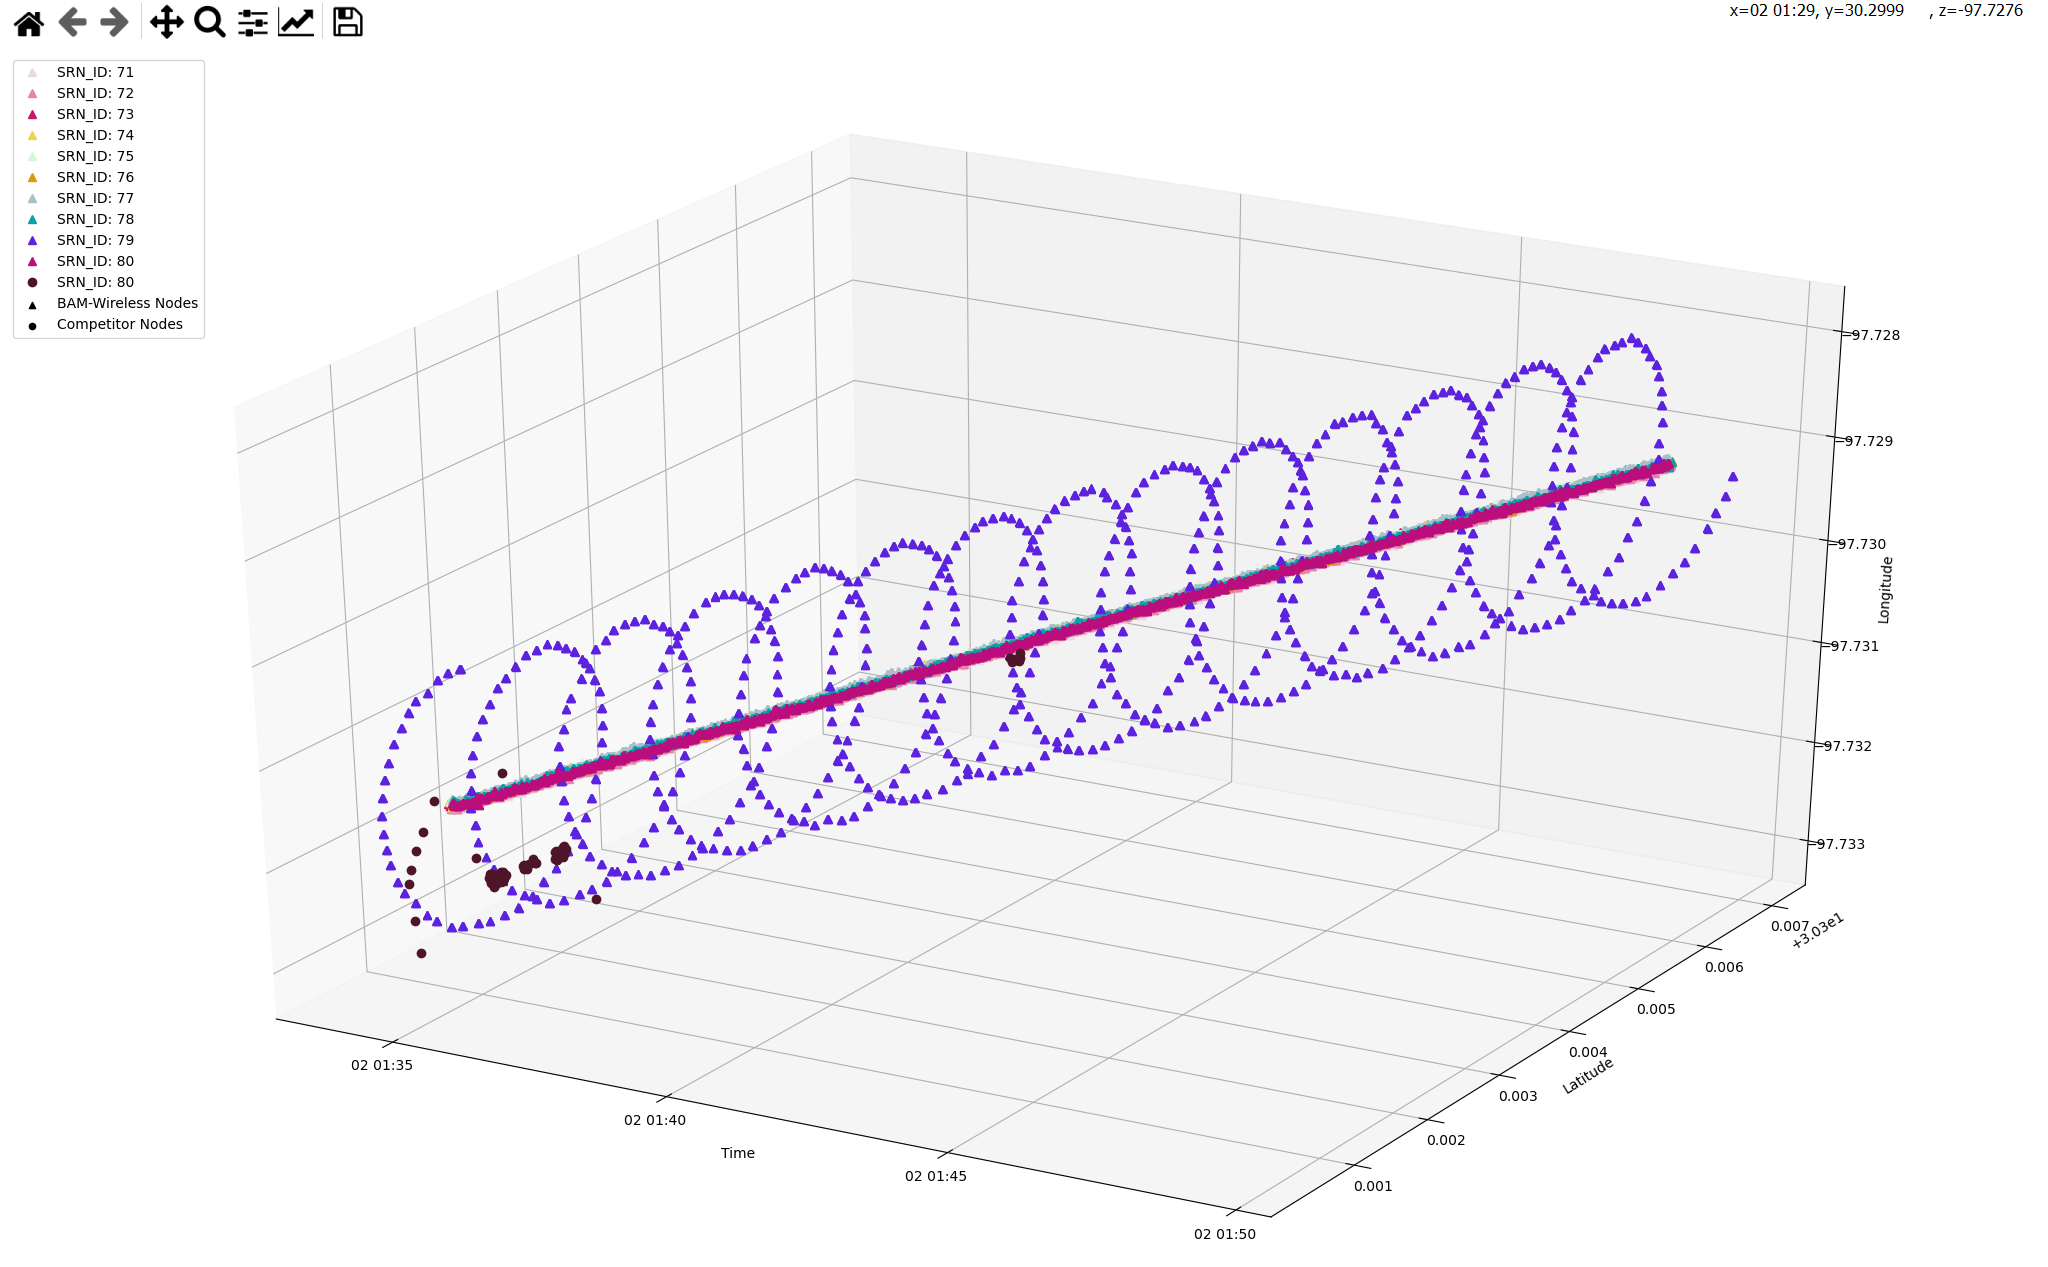
\includegraphics[width = 1.0\textwidth]{Alleys_GPS.PNG}}
    \caption{The reported GPS locations of our SRNs, in addition to those of our competing SRNs, during the Alleys of Austin scenario emulation}
    \label{fig:B.10}
\end{figure}
\begin{figure} [htb]
    \centerline{
    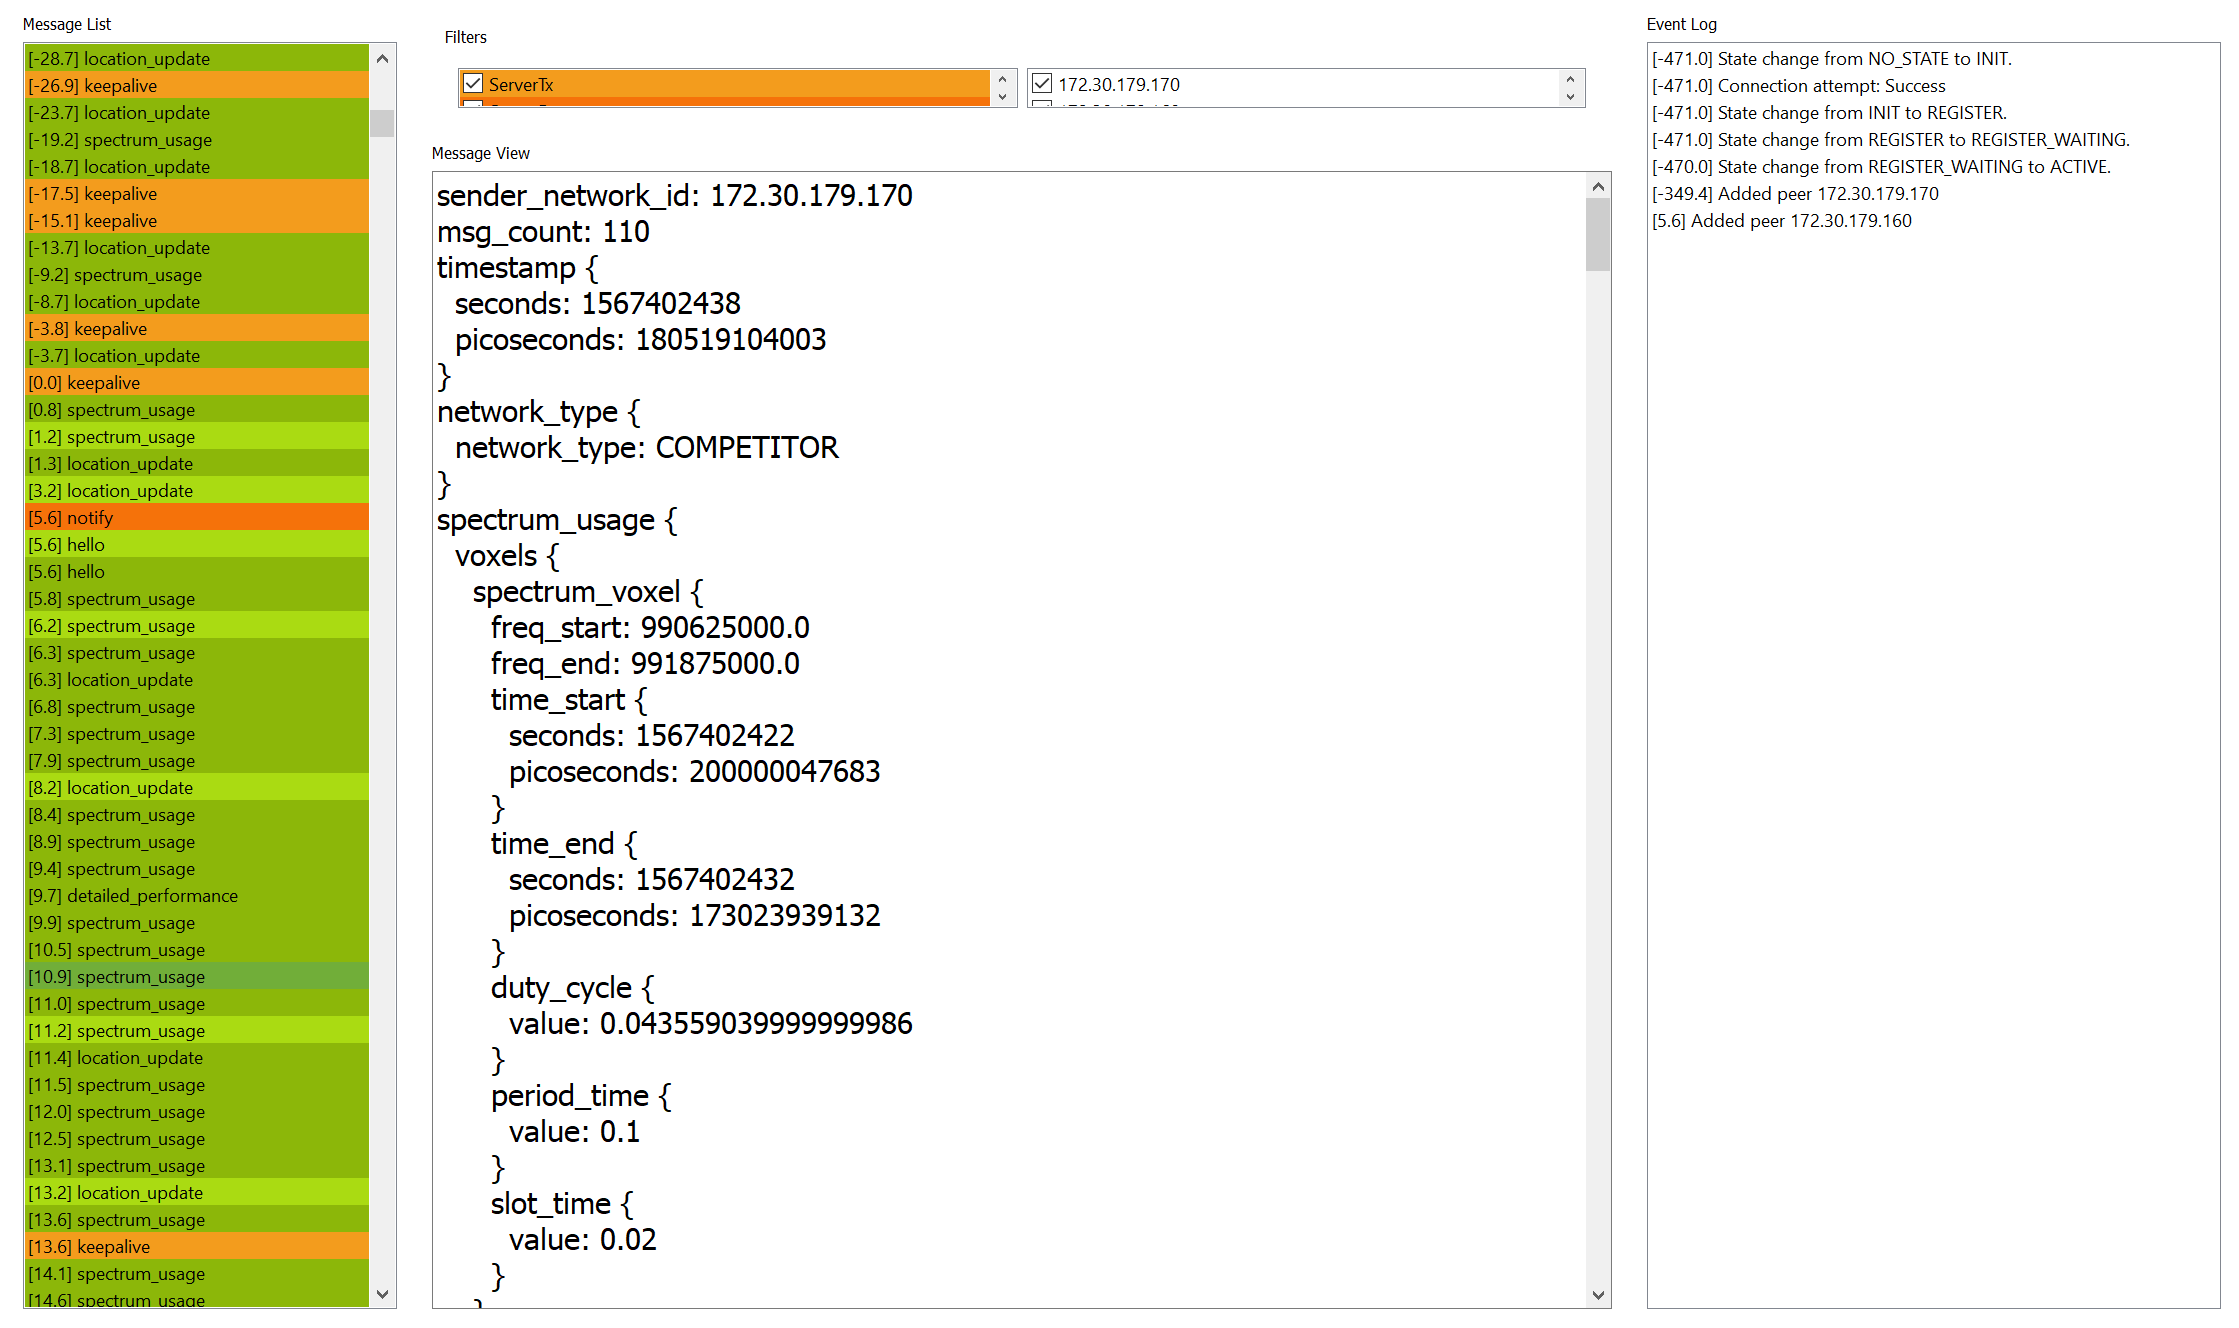
\includegraphics[width = 1.0\textwidth]{Alleys_Collab.PNG}}
    \caption{The description of various CIL message exchanges between our network and the collaboration server, in addition to those between our network and our peers, during the Alleys of Austin scenario emulation}
    \label{fig:B.11}
\end{figure}
\begin{figure} [htb]
    \centerline{
    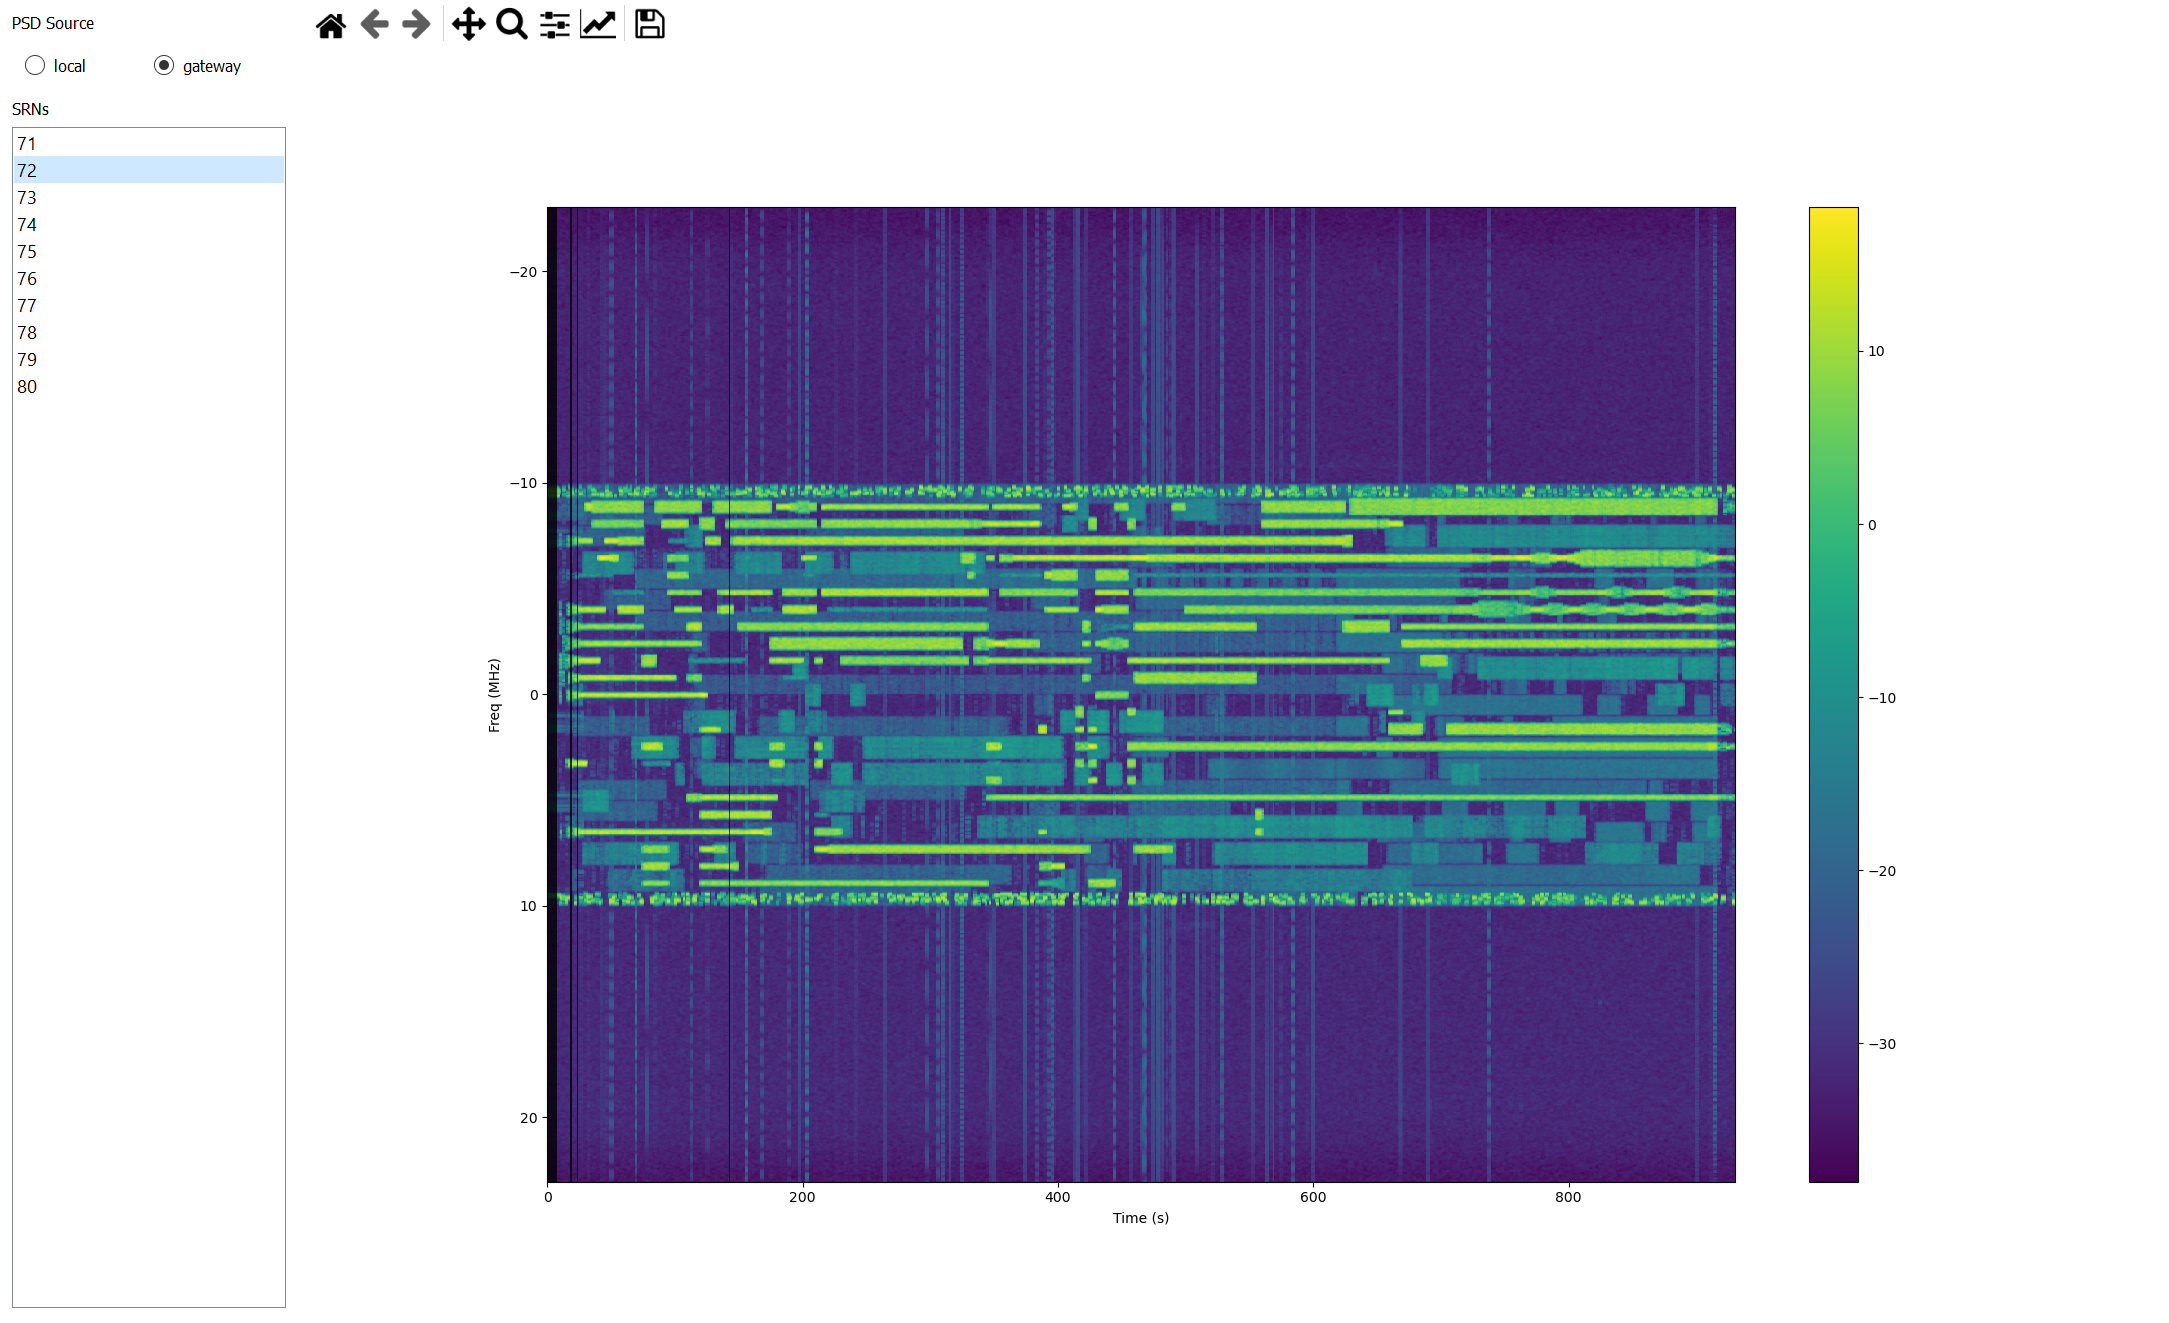
\includegraphics[width = 1.0\textwidth]{Alleys_PSD.PNG}}
    \caption{The PSD measurements received at our Gateway SRN from one particular SRN in our network (selected), in order to obtain location-specific spectrum occupancy information, during the Alleys of Austin scenario emulation}
    \label{fig:B.12}
\end{figure}
\begin{figure} [htb]
    \centerline{
    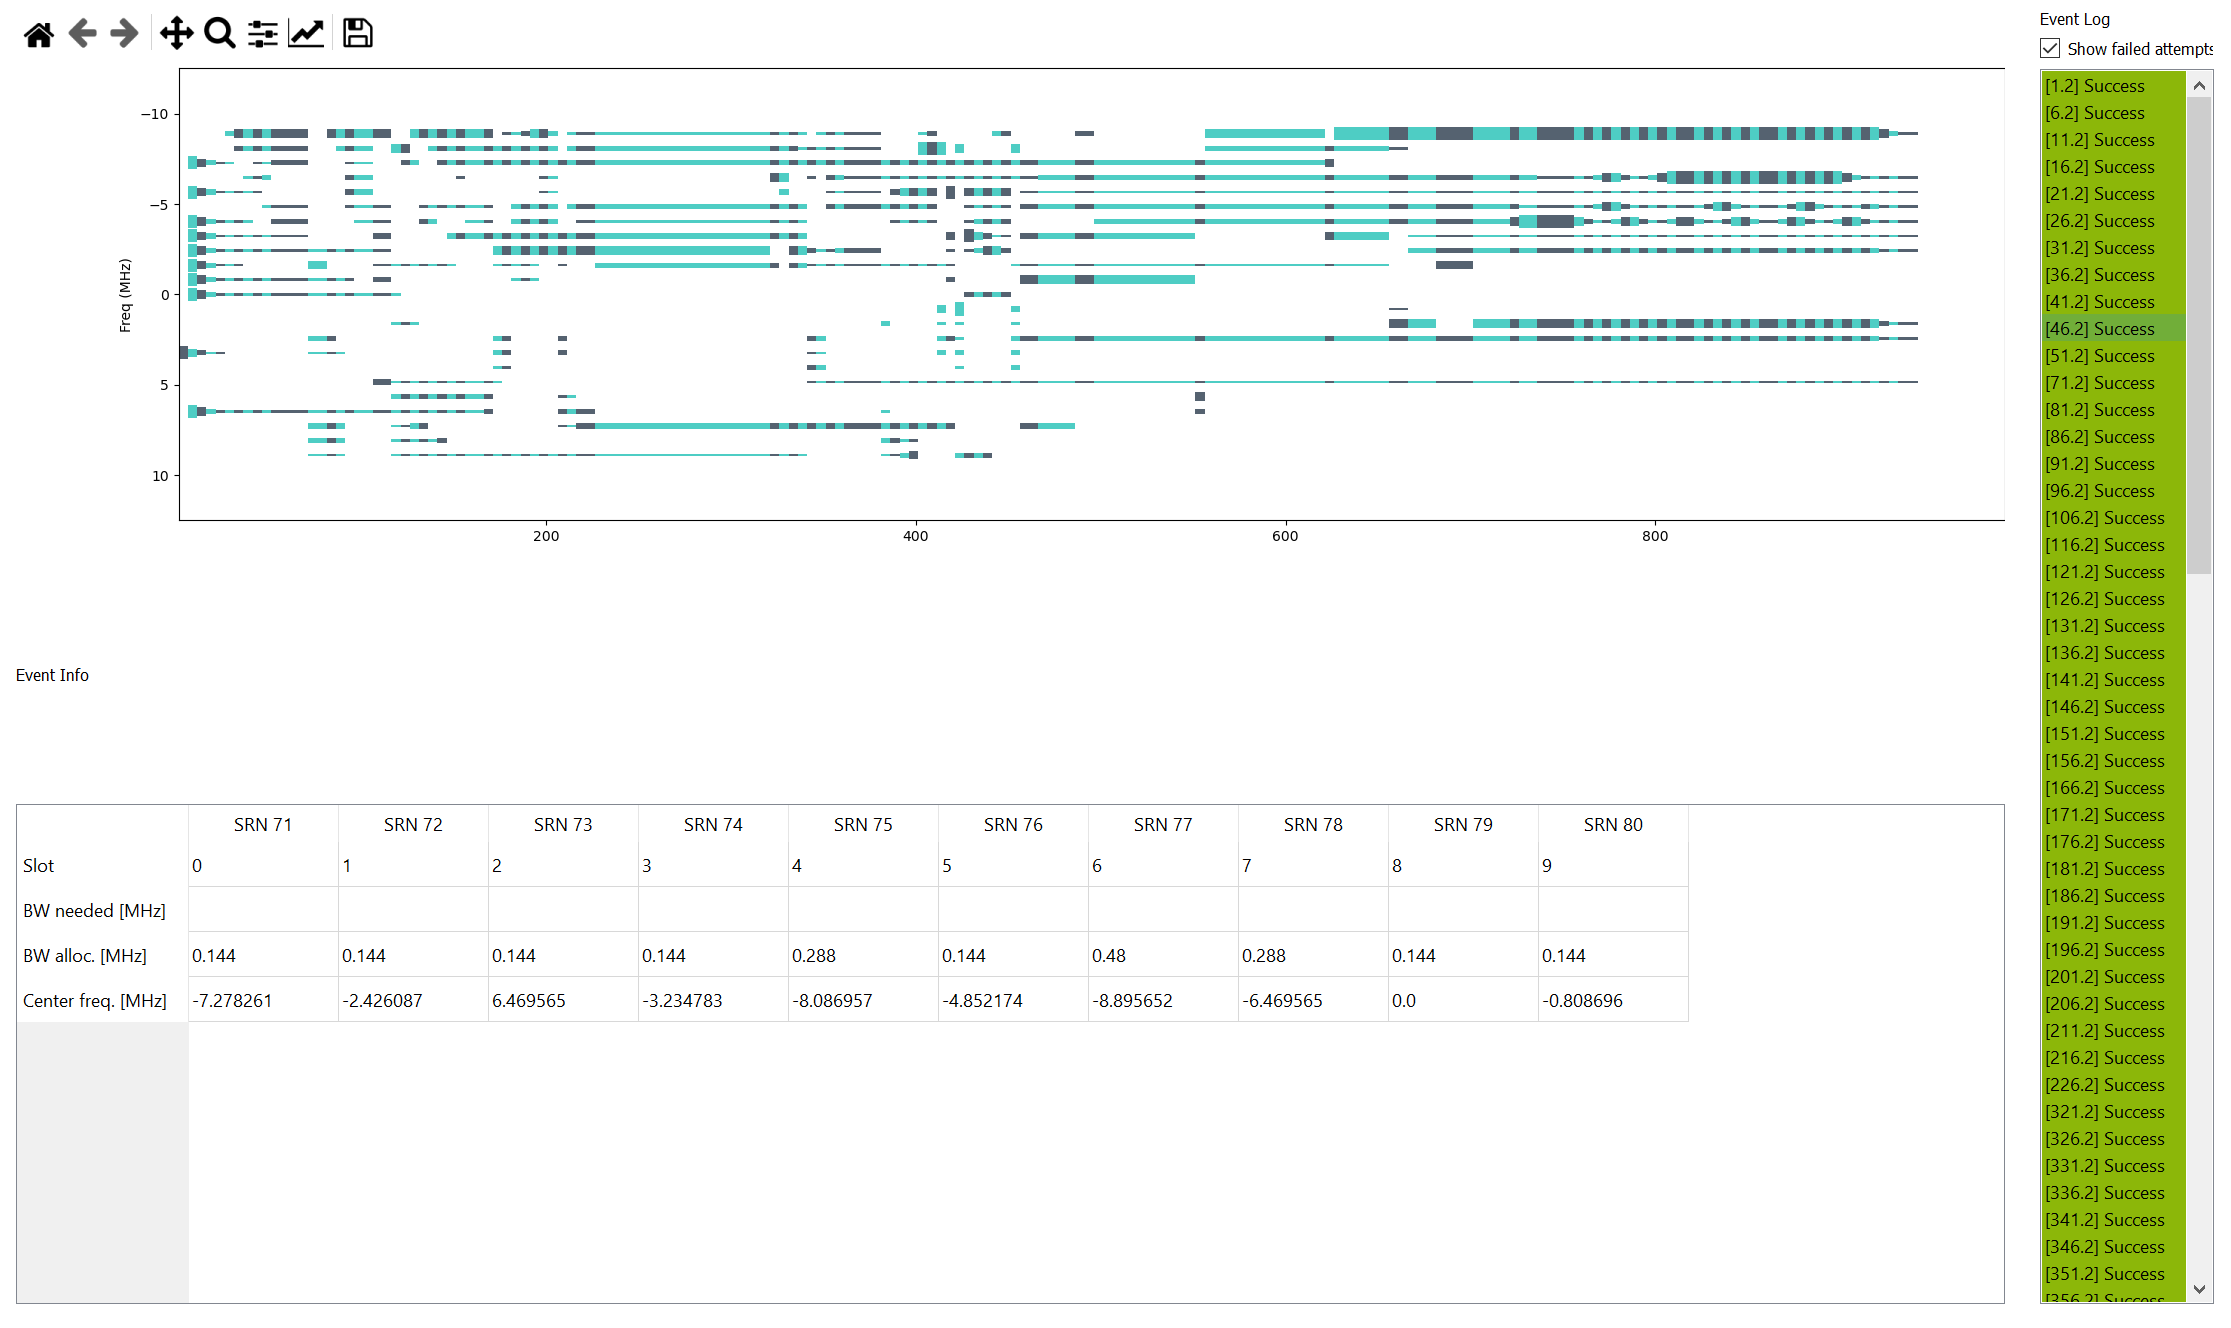
\includegraphics[width = 1.0\textwidth]{Alleys_Channel_Alloc.PNG}}
    \caption{The spectrum occupancy behavior of SRNs in our network (as guided by our Gateway SRN) during the Alleys of Austin scenario emulation}
    \label{fig:B.13}
\end{figure}
The reported GPS locations (latitude, longitude) of the SRNs in our CIRN, and the SRNs in our competitors' CIRNs, over time, are depicted in a $3$-dimensional time plot shown in Fig. \ref{fig:B.10}. The location information of these SRNs\texttt{-{}-}particularly, in relation to physical obstacles (emulated) and competitor SRNs, is employed in the channel allocation algorithm in our Gateway SRN. Fig. \ref{fig:B.11} illustrates the various timestamped CIL messages (both Client-Server messages and Peer-to-Peer messages) received by our Gateway SRN over the collaboration network\texttt{-{}-}these messages are exploited by our Gateway SRN, which along with the collated location-specific PSD measurements: one such PSD measurement in a given time snapshot observed at SRN with ID\texttt{-}$72$ and sent to our Gateway, is depicted in Fig. \ref{fig:B.12}\texttt{-{}-}determines a channel allocation (center frequencies) that minimizes the total interference caused at our SRNs by our competitors. Consequently, from an overall scenario duration perspective, the channel allocations of our network are collated into one ``big-picture" illustration, shown in Fig. \ref{fig:B.13}. It is evident from Fig. \ref{fig:B.13} that in Stage $1$, there are frequent channel re-allocations and bandwidth adjustments, as evidenced by the breaks in the beginning of the plot\texttt{-{}-}this is due to the fact that all the networks, including ours, are trying to find an ``equilibrium" allocation that not only helps them achieve their mandates, but also ensures that the ensemble, as whole, achieves its score threshold; Stage $2$ has a stable channel and bandwidth allocation, as evidenced by the lower number of breaks in the middle of the plot, due to ``equilibrium" being achieved by our network and still a lower amount of traffic, similar in scale to Stage $1$; and finally, in Stage $3$, the significant increase in the offered traffic of all three flows (voice, imagery, and video) places an enormous strain on the limited available RF spectrum allotted for this scenario emulation, and since all teams are vying for the same spectrum resources all the time, due to the increased offered traffic, we see significant breaks towards the end of the plot, indicating frequent bandwidth adjustments and channel re-allocations\texttt{-{}-}this causes poor performance in Stage $3$, as seen in Fig. \ref{fig:B.6} and Fig. \ref{fig:B.9}, but our network still outperforms our competitors in this Stage.
\subsection{Wildfire}
This scenario emulates a disaster-relief deployment\texttt{-{}-}$5$ National Guard units have been deployed to the Lake Sutherland area in Washington in order to fight a wildfire that is raging there. Each of these $5$ National Guard teams are equipped with an Aerostat to assist in communications, and $4$ water-bombers (unmanned water tankers) to put out the blaze. This scenario emulation involves $6$ stages: the water-bombers get into position in Stage $1$; and in Stages $2-6$, $5$ water-bombers from $2$ teams are sent to drop their load onto the blaze, during which these $5$ water-bombers stream high-definition video back (Video\_Bombing\_Run flows\texttt{-}15 points per flow) to the Aerostat (i.e., the unit command and control center), while the remaining loitering $15$ water-bombers send out basic pings to the Aerostat\texttt{-{}-}after dropping their load onto the fire, these $5$ water-bombers come back to their initial position to reload, the next $5$ go out to drop their load, and the process continues until the end of this scenario emulation. Each competitor CIRN represents a National Guard unit\texttt{-{}-}thereby resulting in a $5$ team, $50$ node, large-scale, small packet, disaster-relief deployment scenario, employing a single-tap propagation model \cite{DARPA:SC2scenarios}. Each team must achieve $50$\% of the QoS mandates assigned to it, during the scenario emulation\texttt{-{}-}in a given time snapshot, teams get scores only if every competitor network achieves their corresponding desired performance in that time snapshot, thereby each competitor is incentivized to work with the others in the network in achieving the required mandates. Note here that the main challenge in this scenario emulation is to collaborate with our competitors in this deployment in order to ensure that the ``active" SRNs, i.e., the water-bombers that are sent out to drop their load get most of the spectrum because of the high-definition video flows communicated by these ``active" water-bombers to the Aerostat, are emulated/modeled to need ${\sim}20$\% of the total allocated scenario bandwidth\texttt{-{}-}therefore, teams must work together to facilitate efficient allocation of resources to these ``active" SRNs in any given time snapshot \cite{DARPA:SC2scenarios}.
\begin{figure} [htb]
    \centerline{
    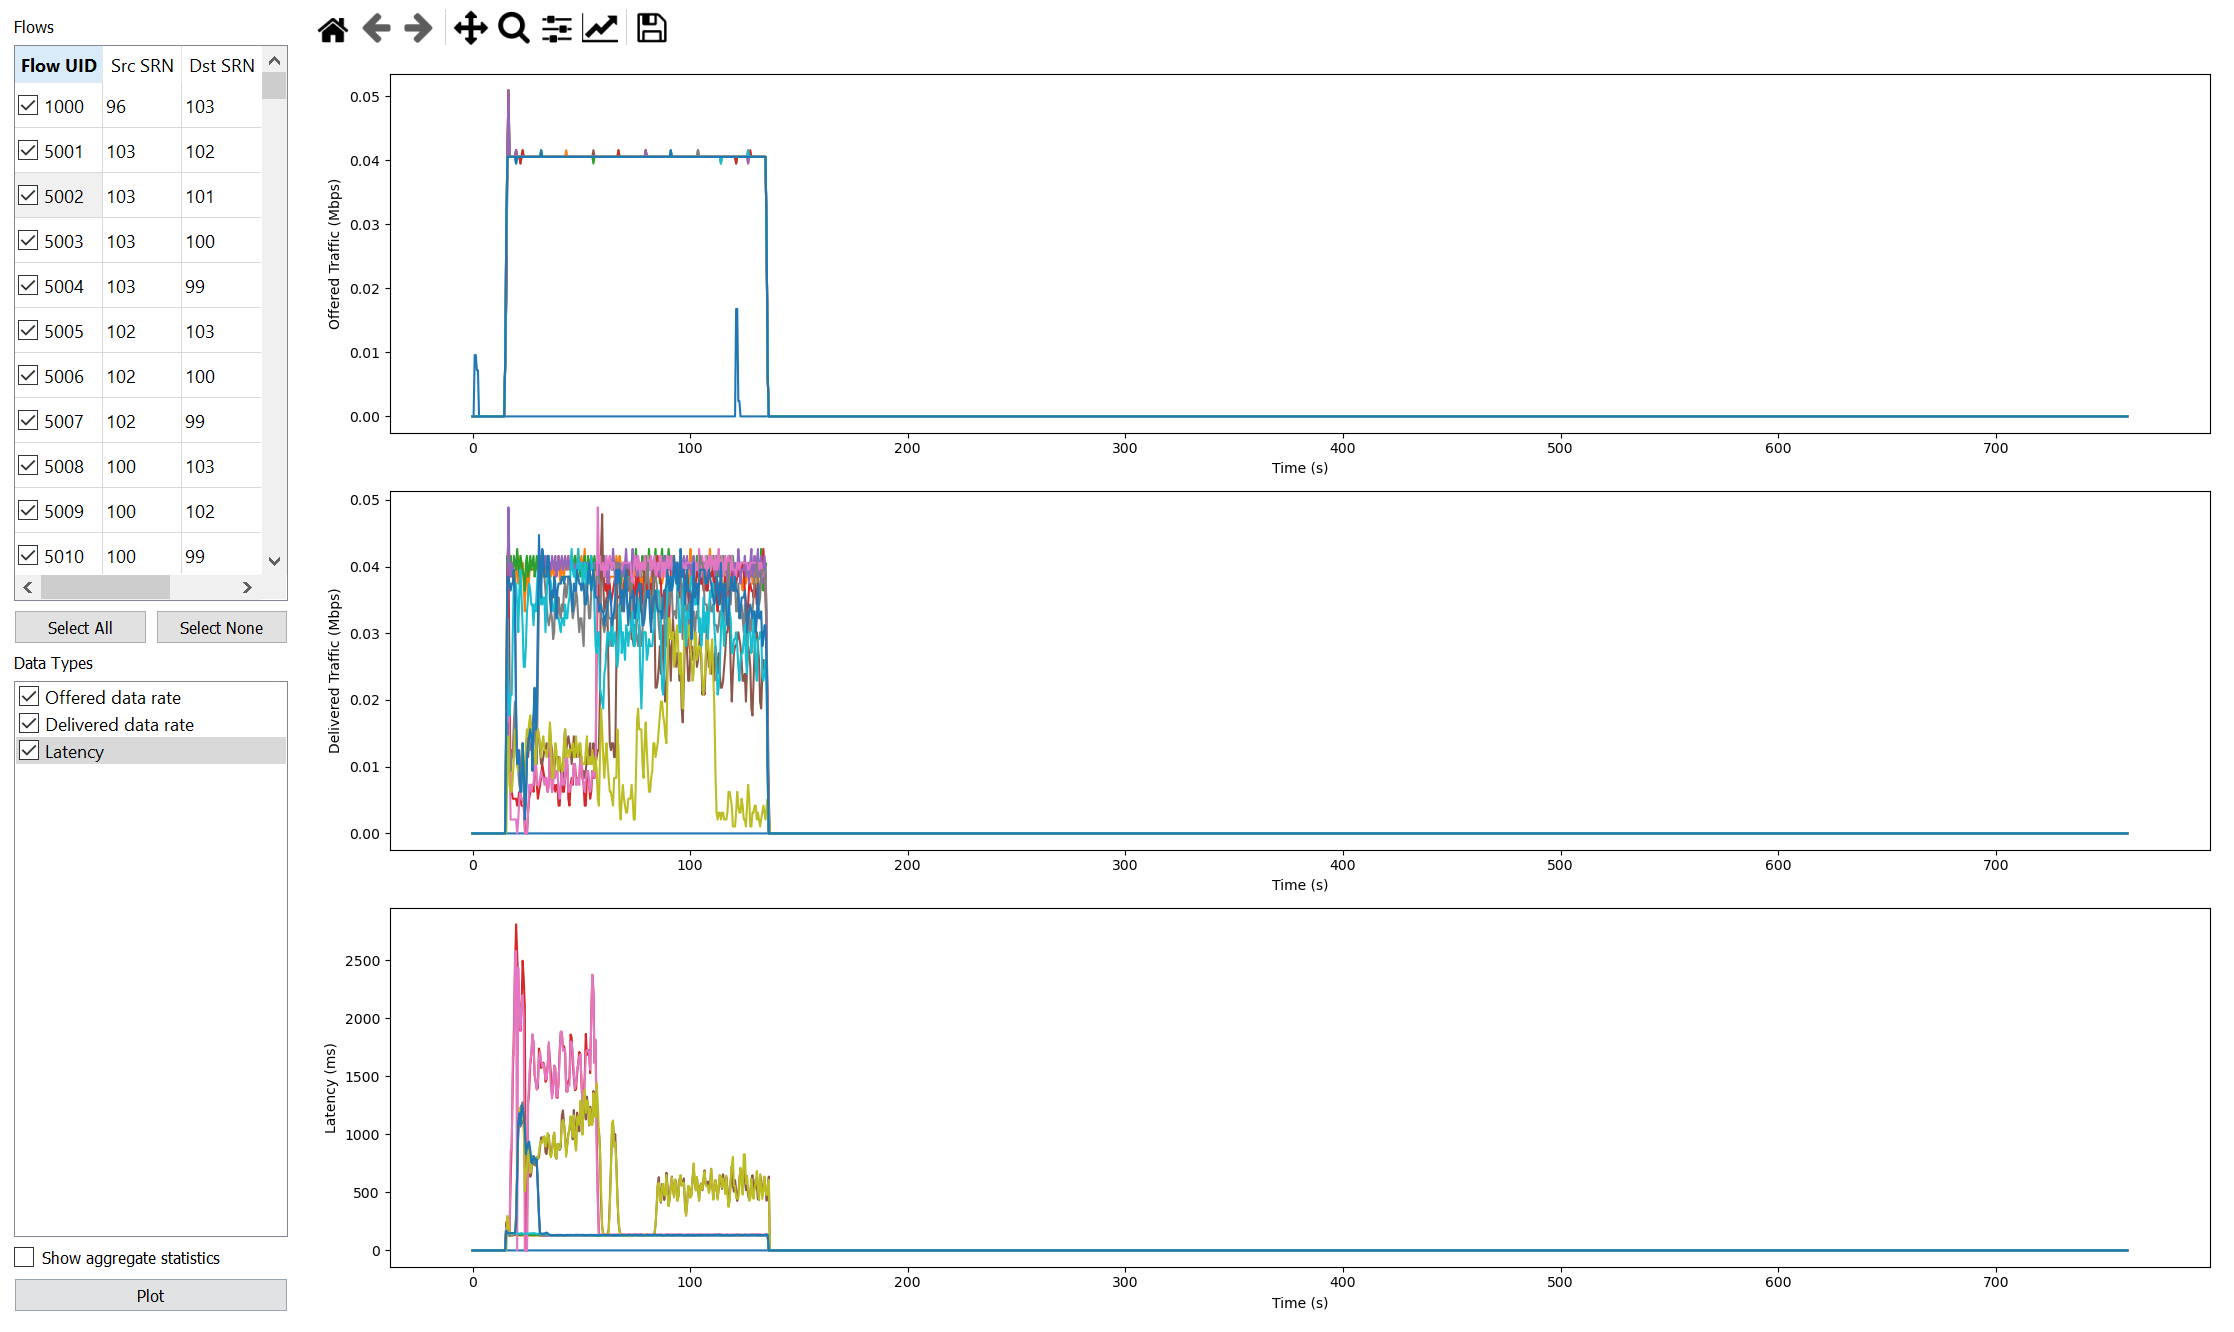
\includegraphics[width = 1.0\textwidth]{Wildfire_NET.PNG}}
    \caption{The offered and delivered traffic corresponding to various (selected) links during the Wildfire scenario emulation (Stage $1$)}
    \label{fig:B.14}
\end{figure}
\begin{figure} [htb]
    \centerline{
    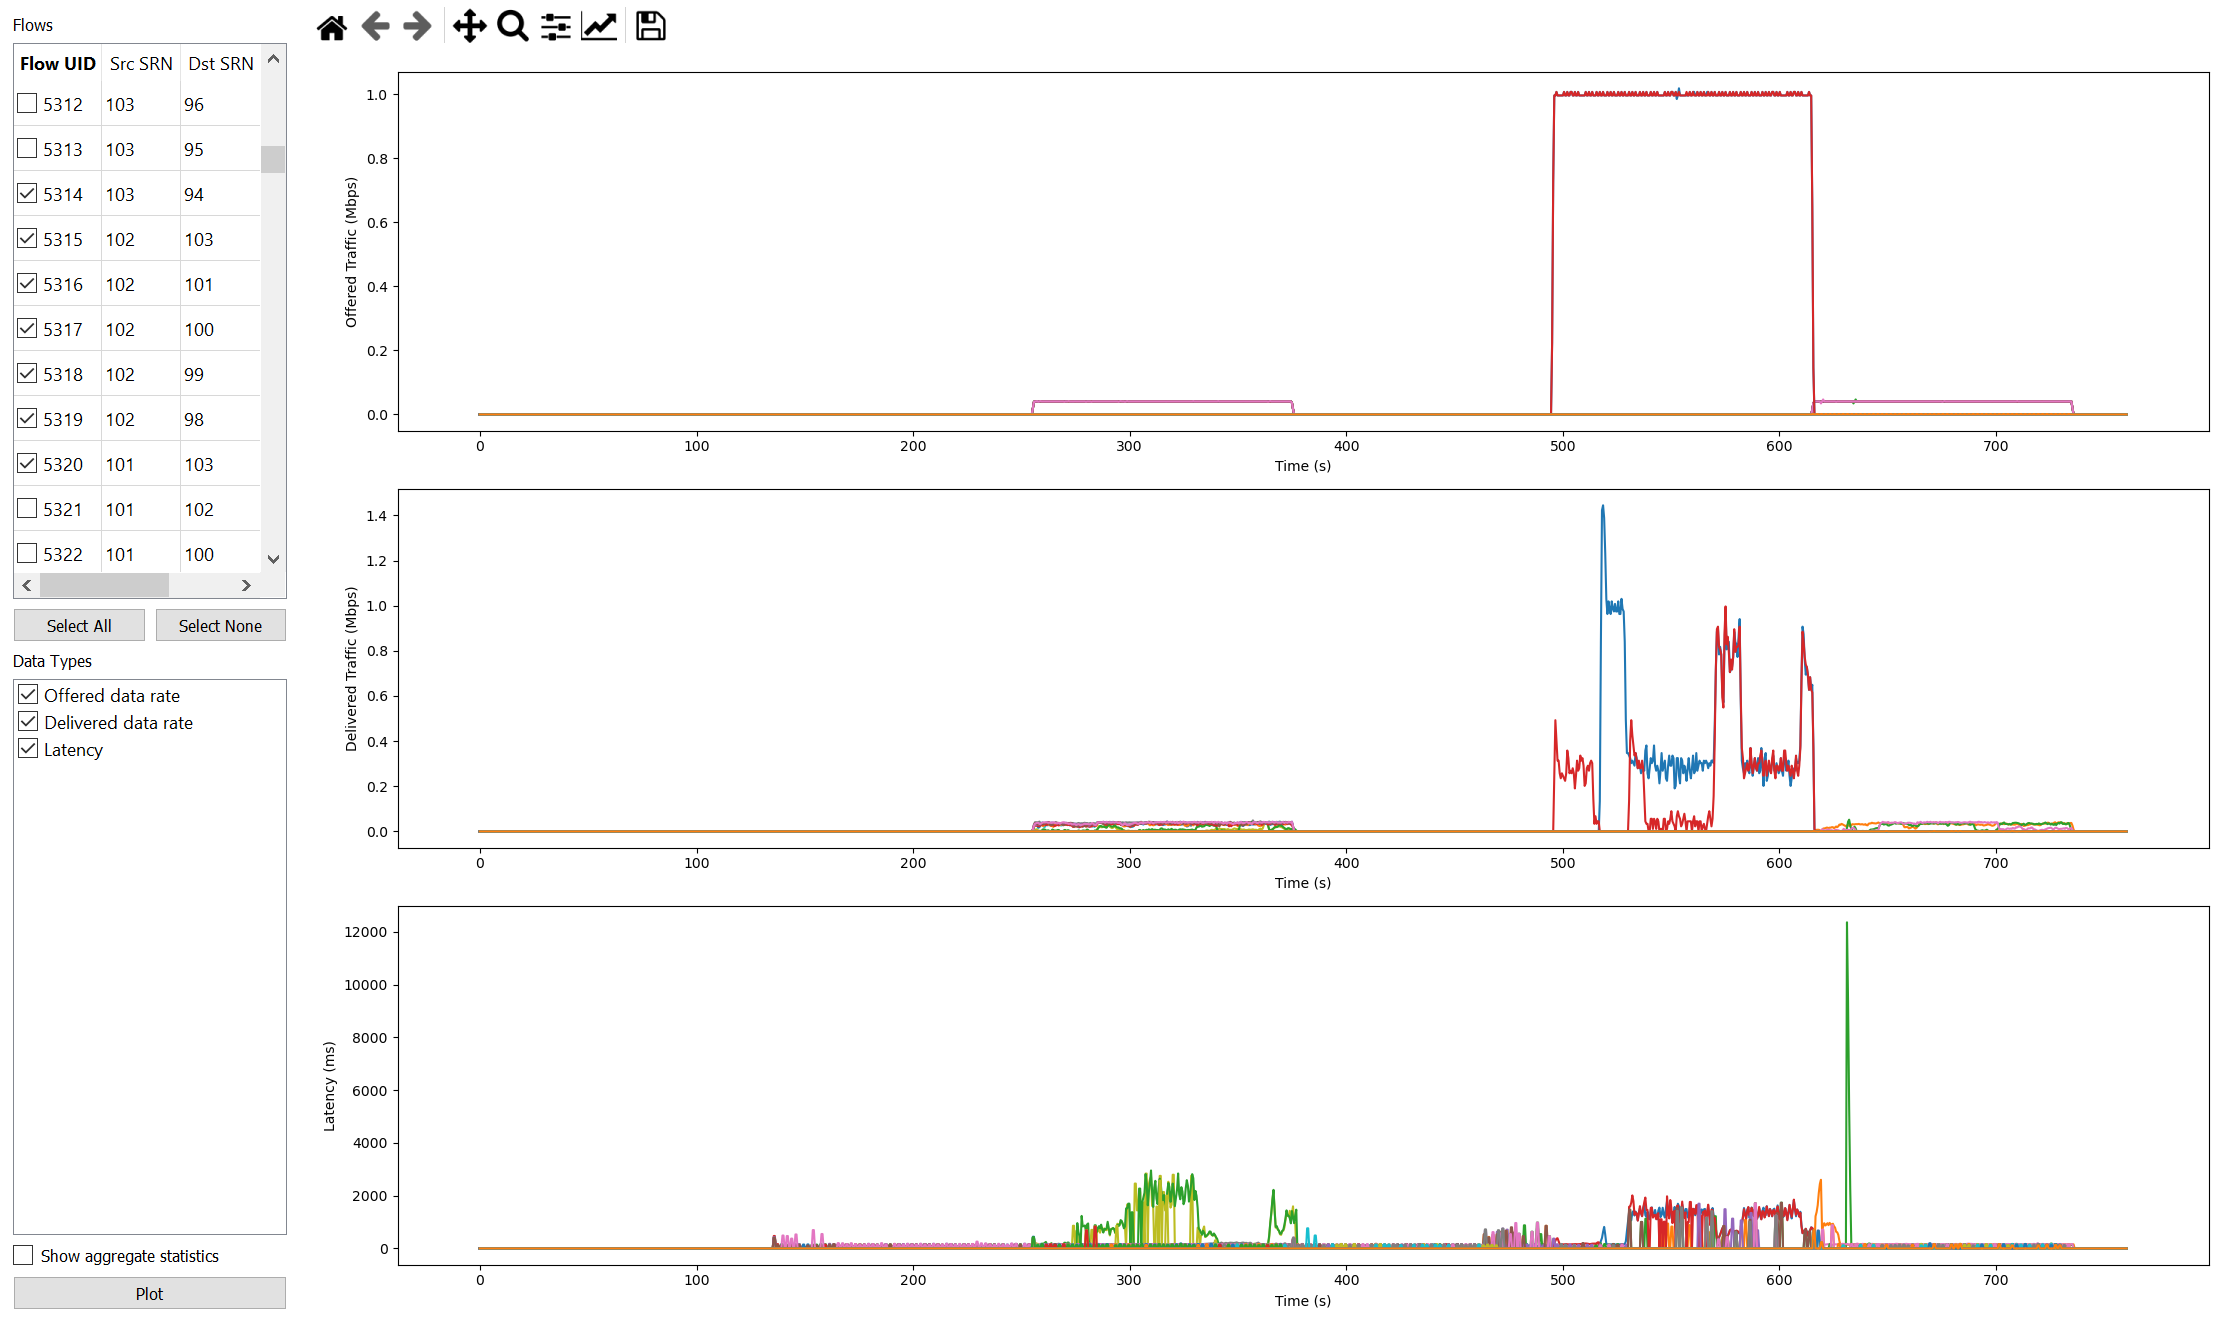
\includegraphics[width = 1.0\textwidth]{Wildfire_NET_2.PNG}}
    \caption{The offered and delivered traffic corresponding to various (selected) links during the Wildfire scenario emulation (Stage $5$)}
    \label{fig:B.15}
\end{figure}

Figs. \ref{fig:B.14} and Fig. \ref{fig:B.15} illustrate the offered traffic corresponding to the individual selected flows, their corresponding delivered traffic, and the latency experienced by these flows as they are being scheduled/delivered by our network, with respect to Stage $1$ and Stage $5$ of the scenario emulation, respectively. Note here that our network is able to deliver almost all of these flows with minimal latency.
\begin{figure} [htb]
    \centerline{
    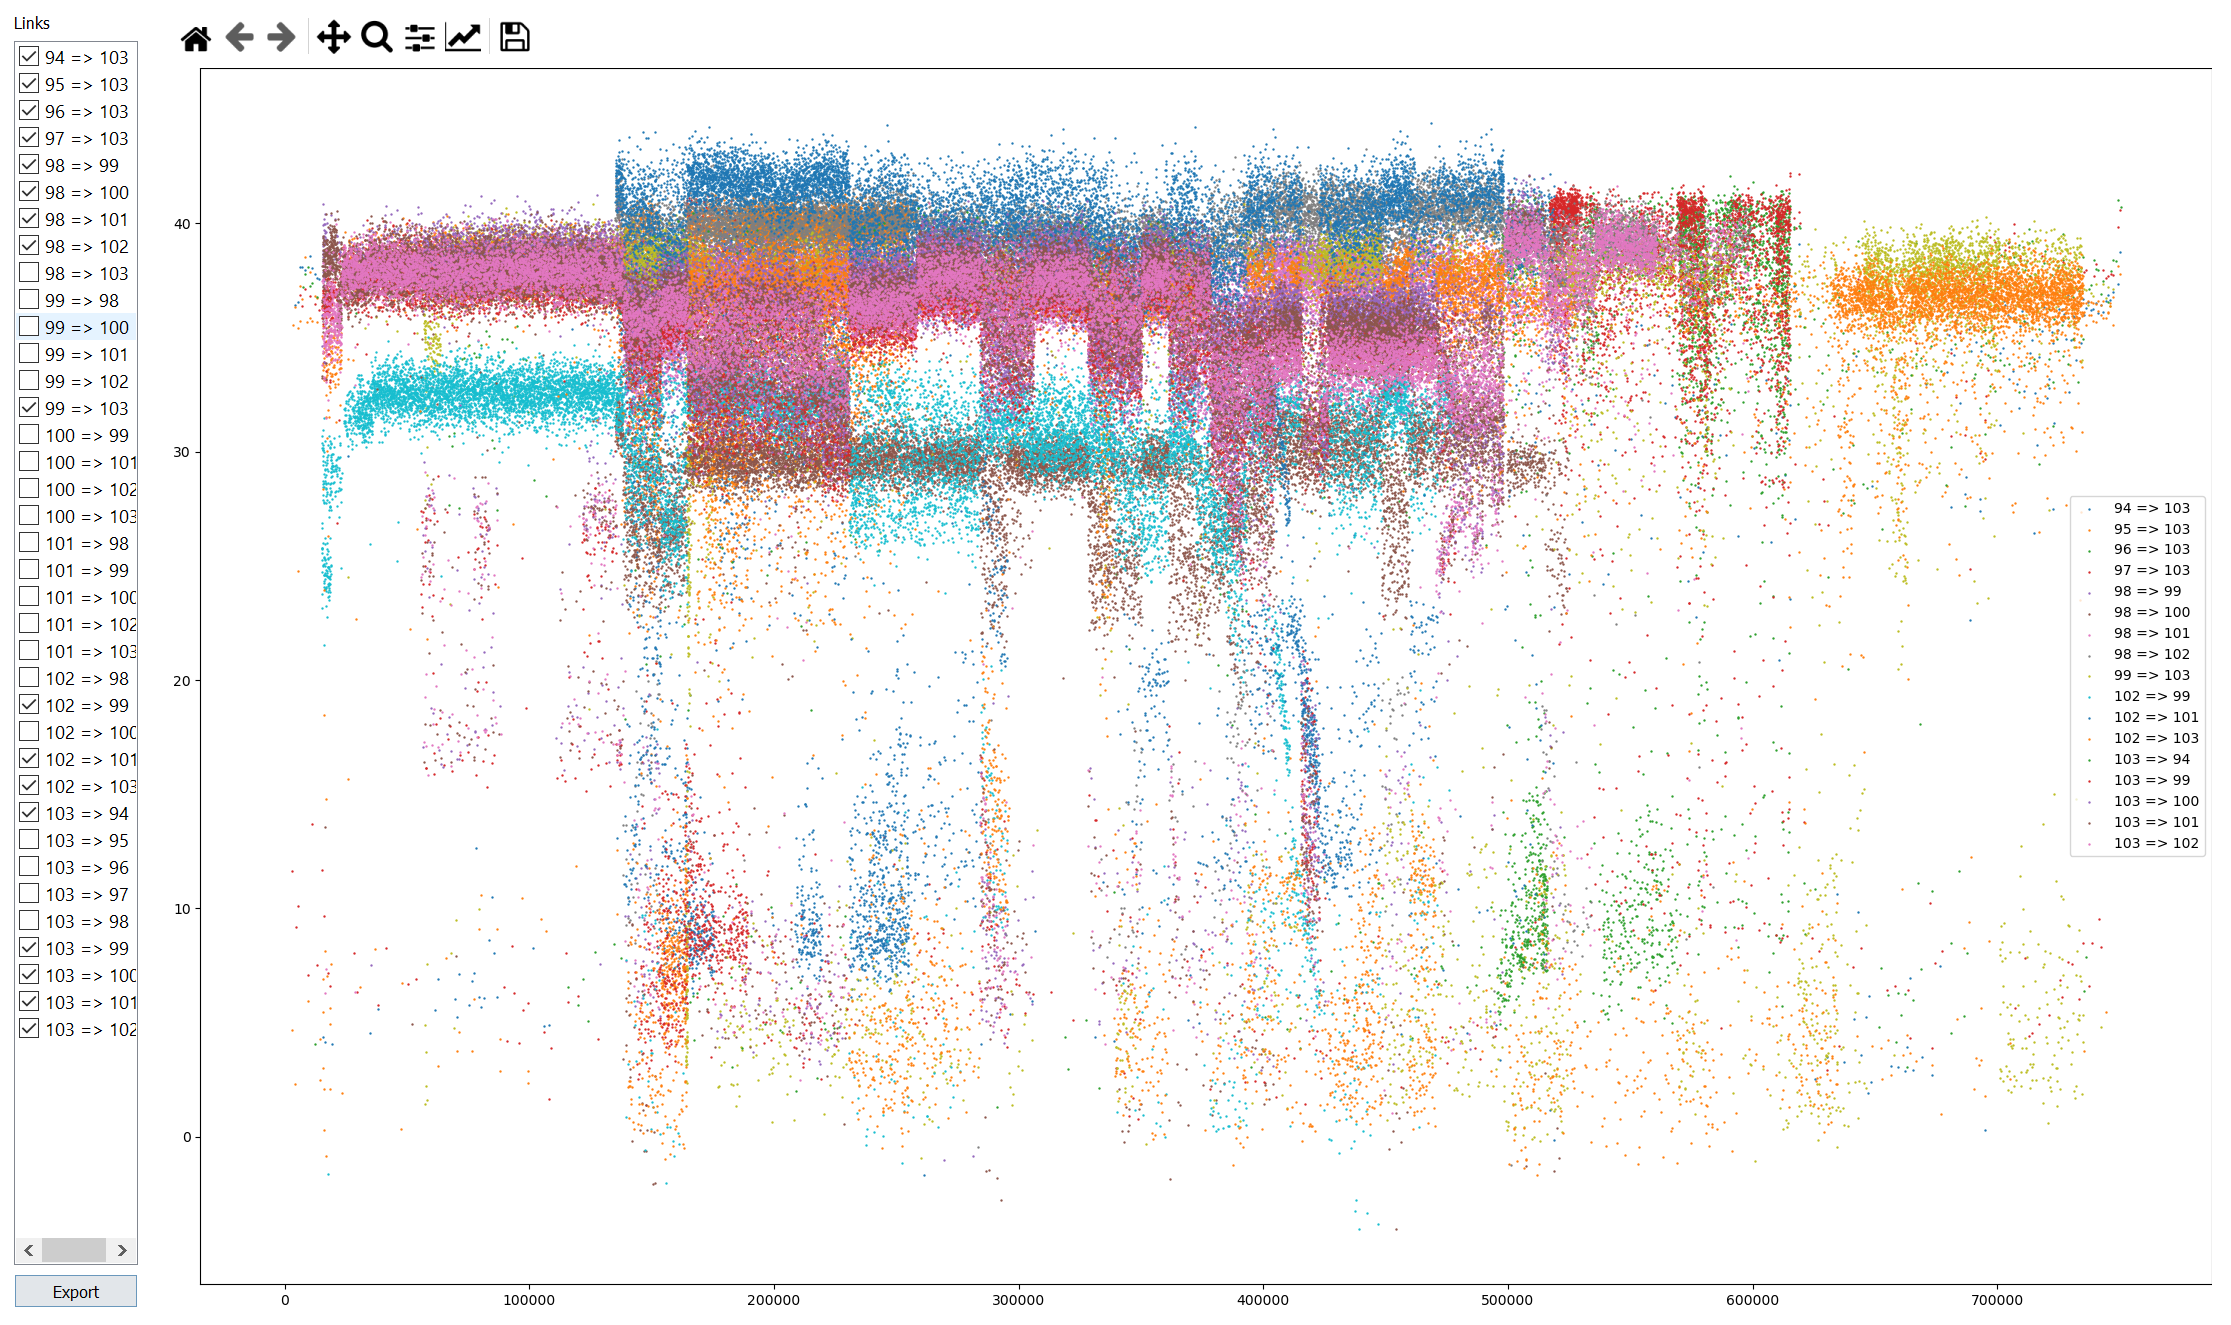
\includegraphics[width = 1.0\textwidth]{Wildfire_SNR.PNG}}
    \caption{The estimated SNR on various (selected links) during the Wildfire scenario emulation}
    \label{fig:B.16}
\end{figure}
\begin{figure} [htb]
    \centerline{
    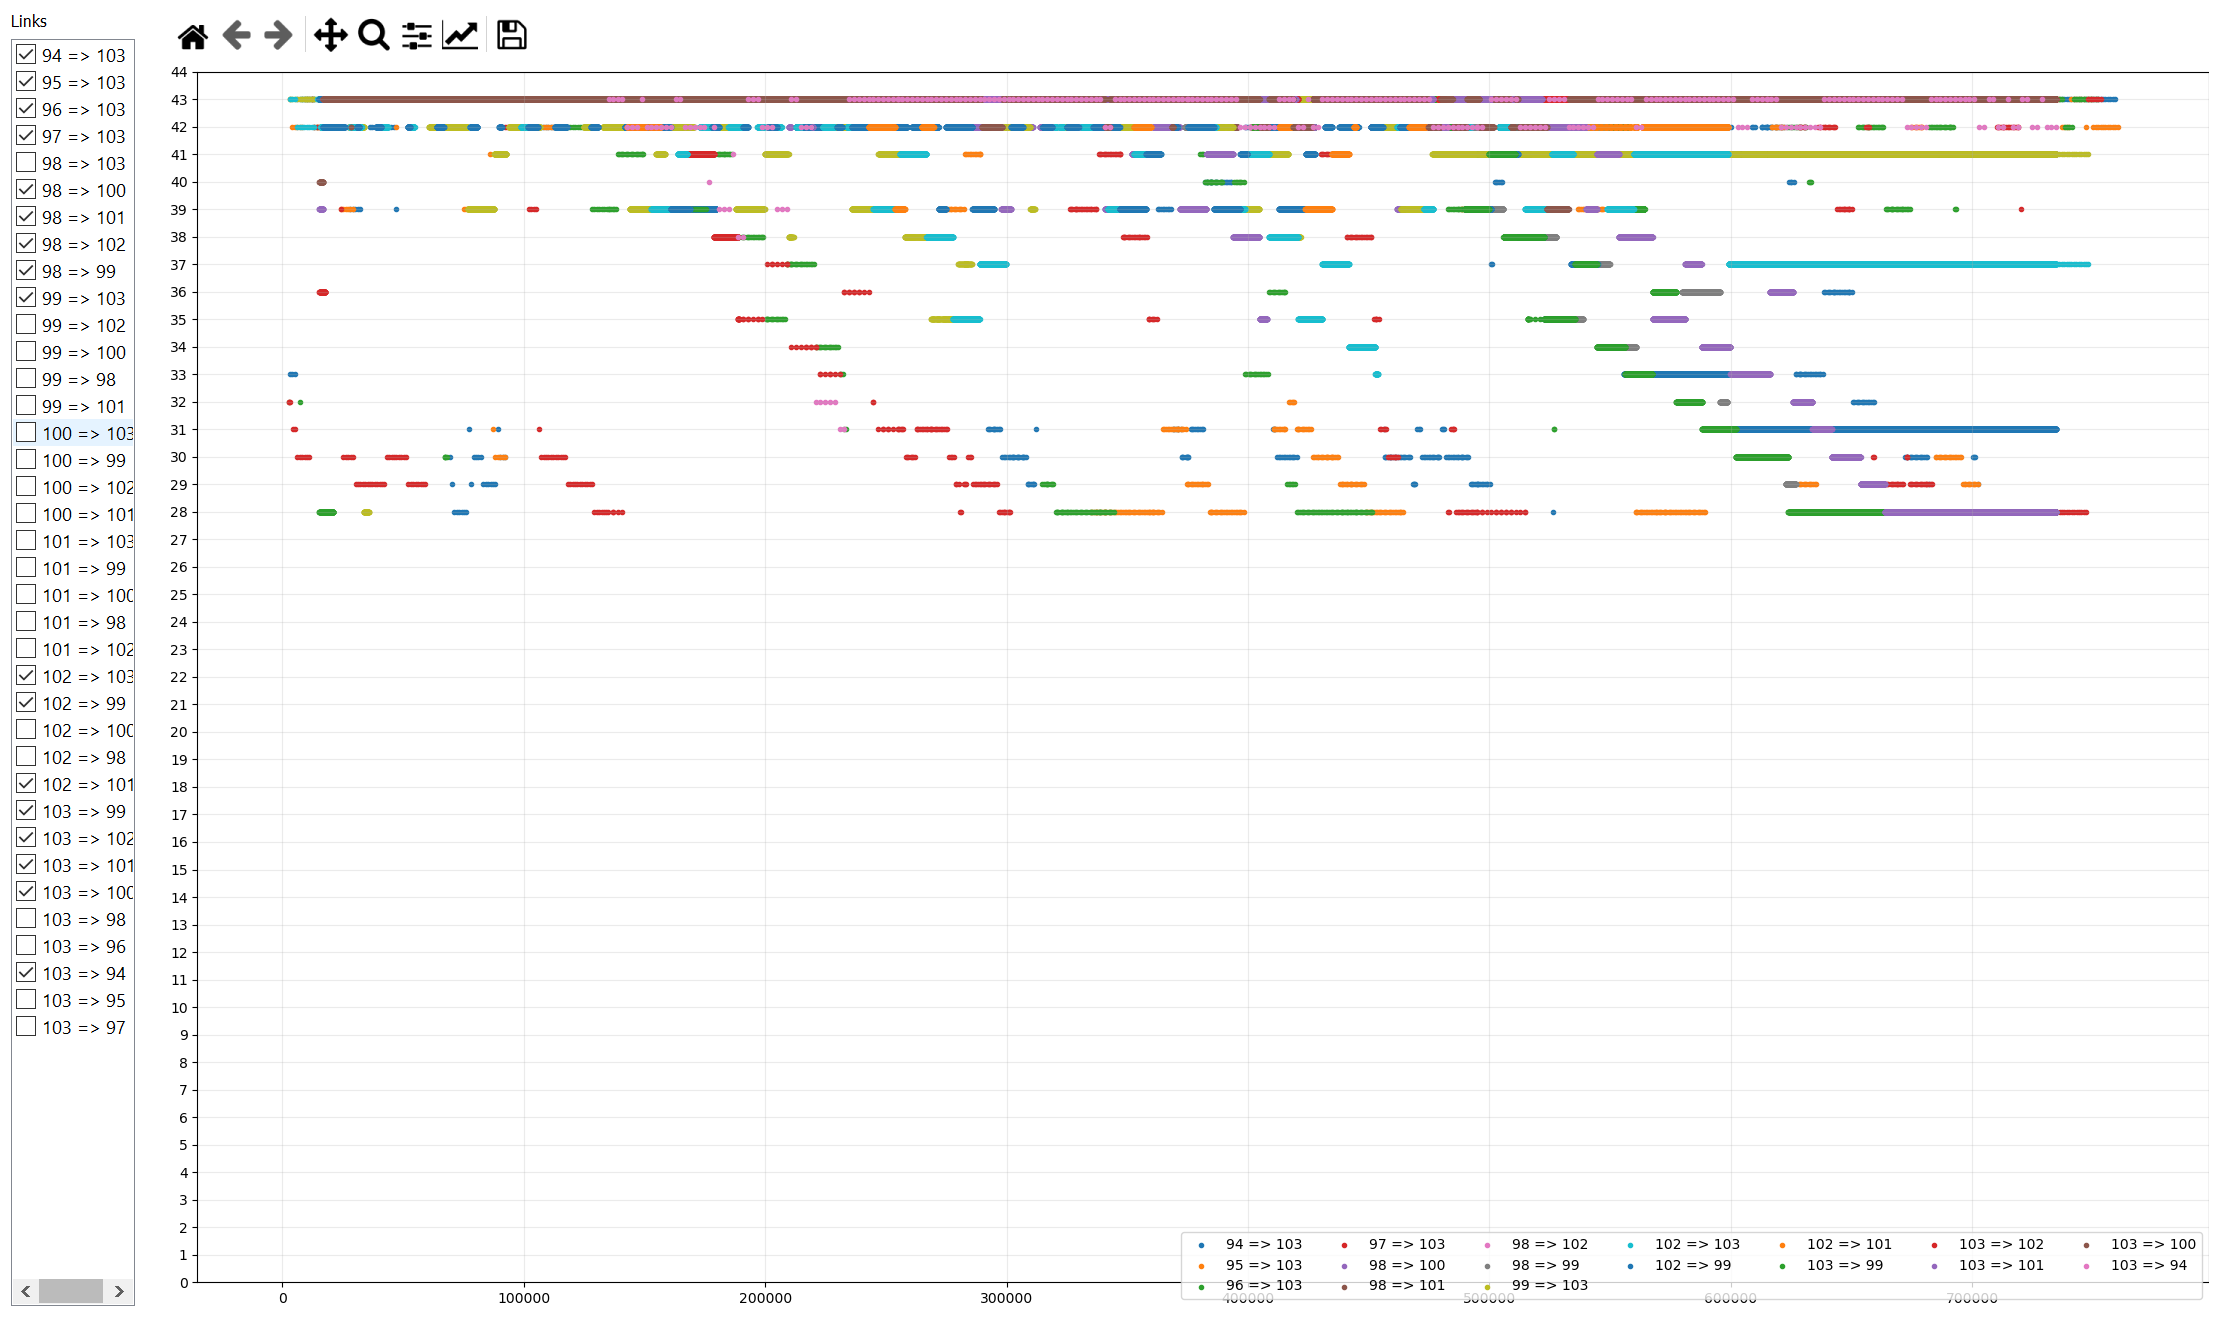
\includegraphics[width = 1.0\textwidth]{Wildfire_MCS.PNG}}
    \caption{The MCS adaptation scheme at each (selected) link during the Wildfire scenario emulation}
    \label{fig:B.17}
\end{figure}

Fig. \ref{fig:B.16} depicts the estimated SNR on various selected links (source SRN - destination SRN), during the progression of the Wildfire scenario\texttt{-{}-}these SNR estimates at each link are, as discussed earlier, employed in the MCS adaptation scheme, the prioritized flow scheduler, and the bandwidth allocation algorithm. Consequently, Fig. \ref{fig:B.17} depicts the MCS adaptation scheme at each of these selected links, adapting to the changing estimated SNR with respect to the corresponding channels used by these links\texttt{-{}-}the Y-axis of the MCS adaptation plot in Fig. \ref{fig:B.17} refers to the C${++}$ enumeration value corresponding to the $(\mathcal{M},\mathcal{R})$ pair, i.e., for example, $43$ in the plot refers to QAM$64$ modulation with a code rate of $\frac{5}{6}$, while $28$ refers to QPSK modulation with $\frac{1}{2}$ code rate\texttt{-{}-}in other words, the highest modulation order used in this Wildfire run is $\mathcal{M}{=}64$ (i.e., QAM$64$), while the lowest modulation order used in $\mathcal{M}{=}4$ (i.e., QPSK).
\begin{figure} [htb]
    \centerline{
    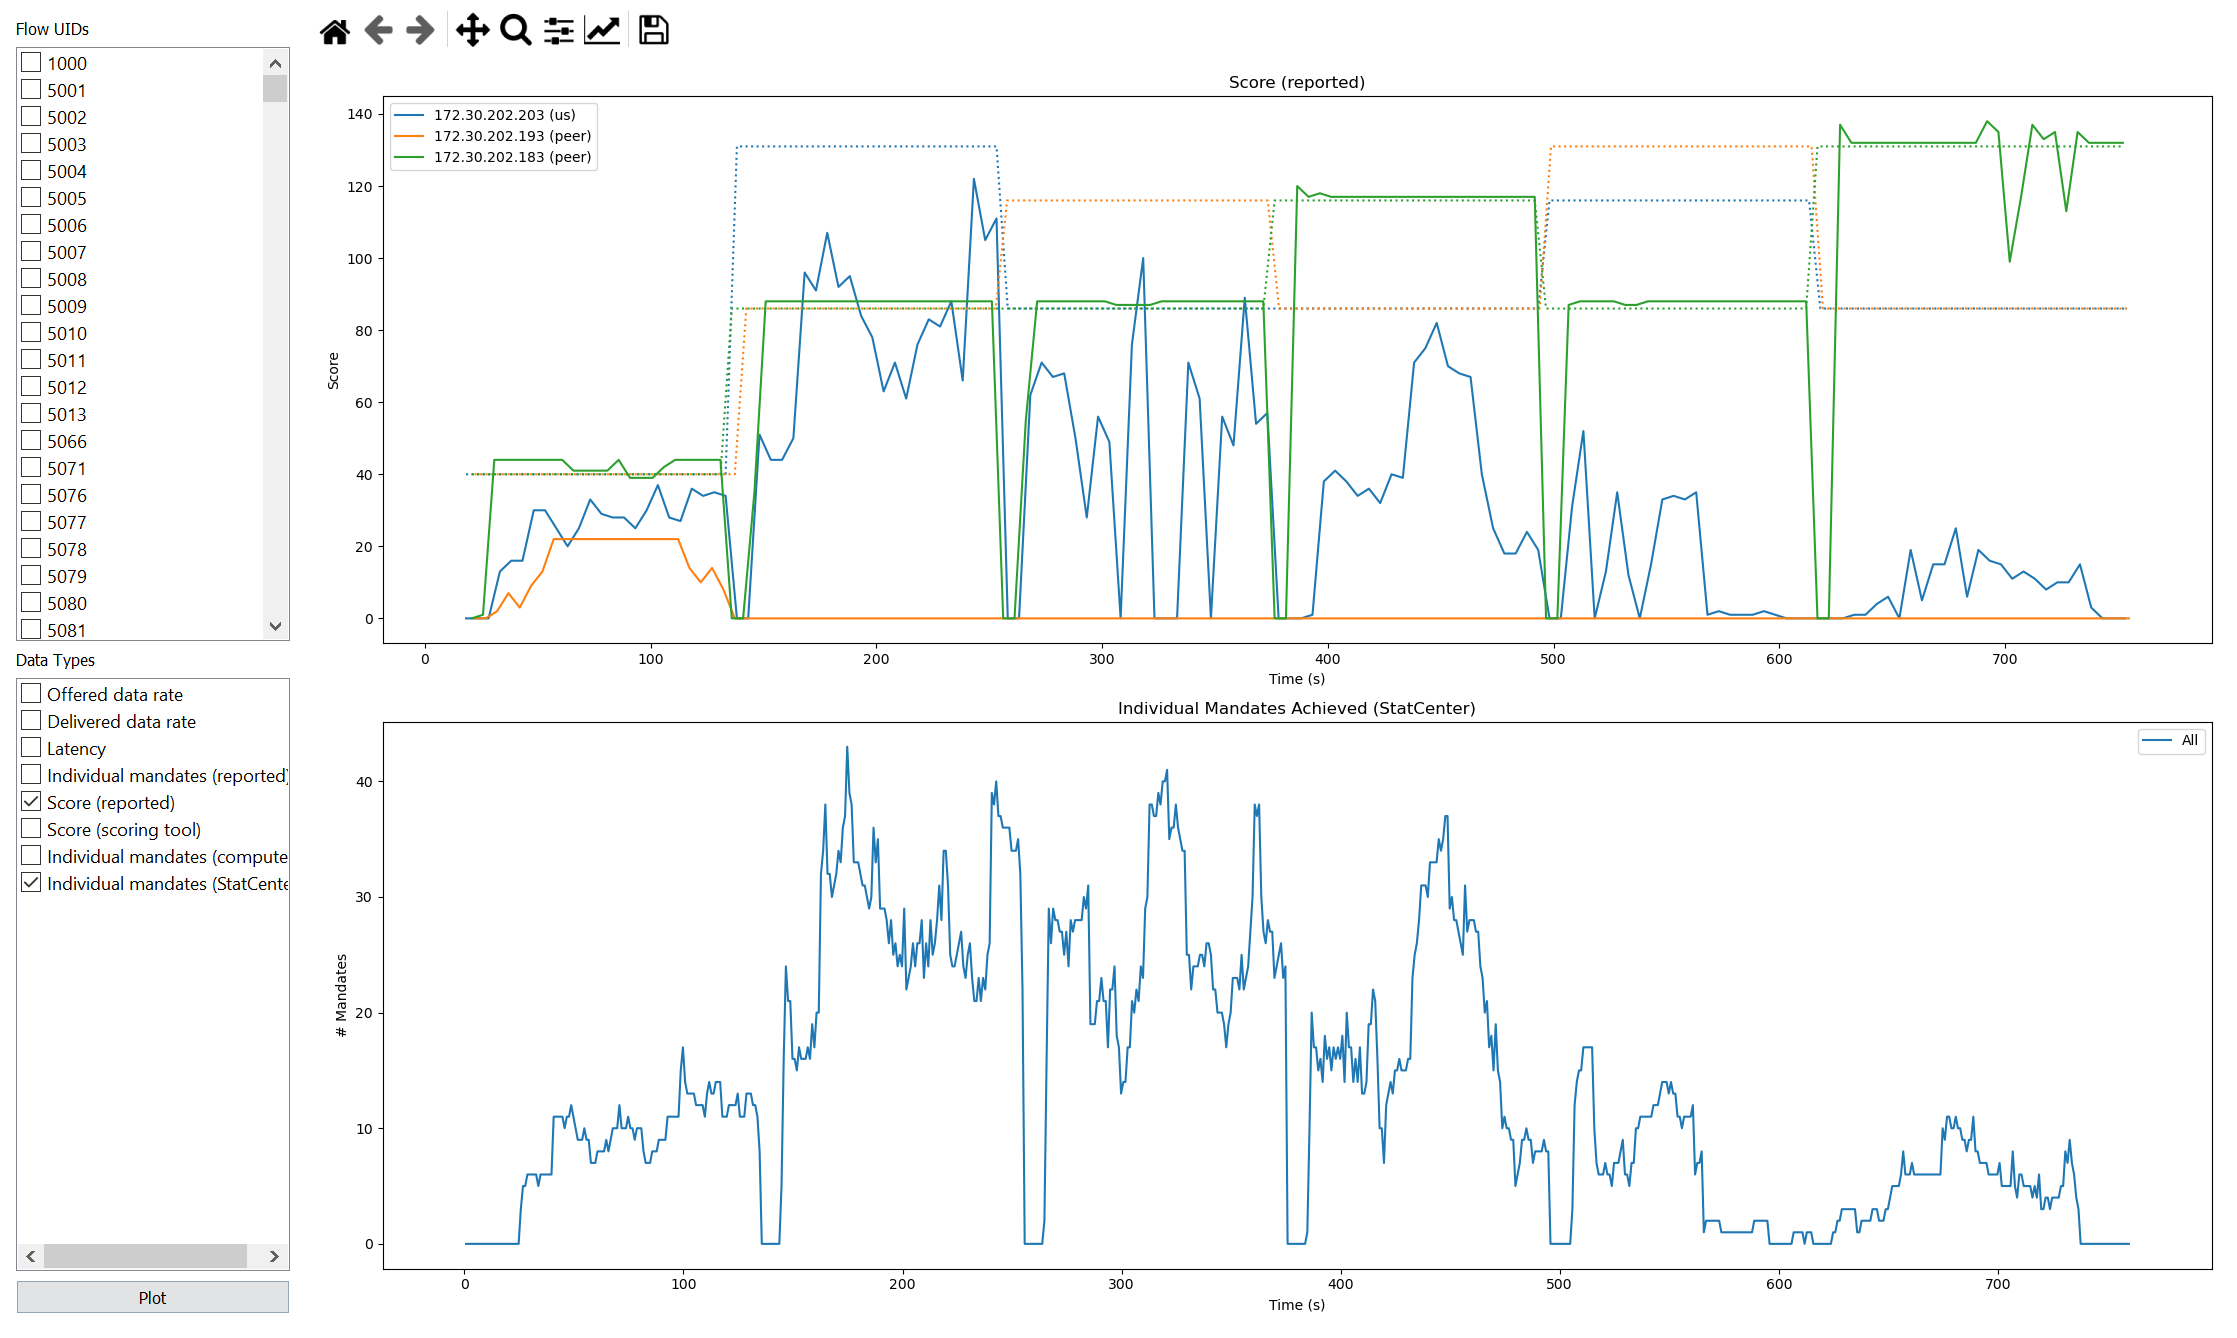
\includegraphics[width = 1.0\textwidth]{Wildfire_Scoring.PNG}}
    \caption{The scores attained by our network and other competing networks during the Wildfire scenario emulation, in addition to the number of QoS mandates satisfied by our network in a given time snapshot}
    \label{fig:B.18}
\end{figure}

Fig. \ref{fig:B.18} illustrates the score obtained by our network (indicated by our Gateway SRN's IP address) along with the scores obtained by our peers (indicated by the IP addresses of their corresponding gateway SRNs) in the scenario emulation. The dotted lines in the first sub-plot indicate the score thresholds that need to be achieved by each network, in a Stage. The second sub-plot illustrates the number of flow-specific QoS mandates that were achieved by our network in a given time snapshot. As evident from the figure, our peer with IP address identifier $172.30.202.183$ performs better than our network, while the other peer with IP address identifier $172.30.202.193$ performs poorly throughout the scenario emulation. Note here that, our network performs quite well in Stages $1$, $2$, and $3$, with our scores above the performance threshold most of time during these initial $3$ stages\texttt{-{}-}however, in Stages $4$, $5$, and $6$, frequent MCS pair switching (adaptation and re-adaptation) as seen in Fig. \ref{fig:B.17}, possibly triggered by poor link quality at a significant number of SRNs (possibly due to aggressive interference from competitor SRNs\texttt{-{}-}specifically, the SRNs from CIRN $172.30.202.183$), causes our performance to deteriorate significantly\texttt{-}leading to scores below the threshold in these stages.
\begin{figure} [htb]
    \centerline{
    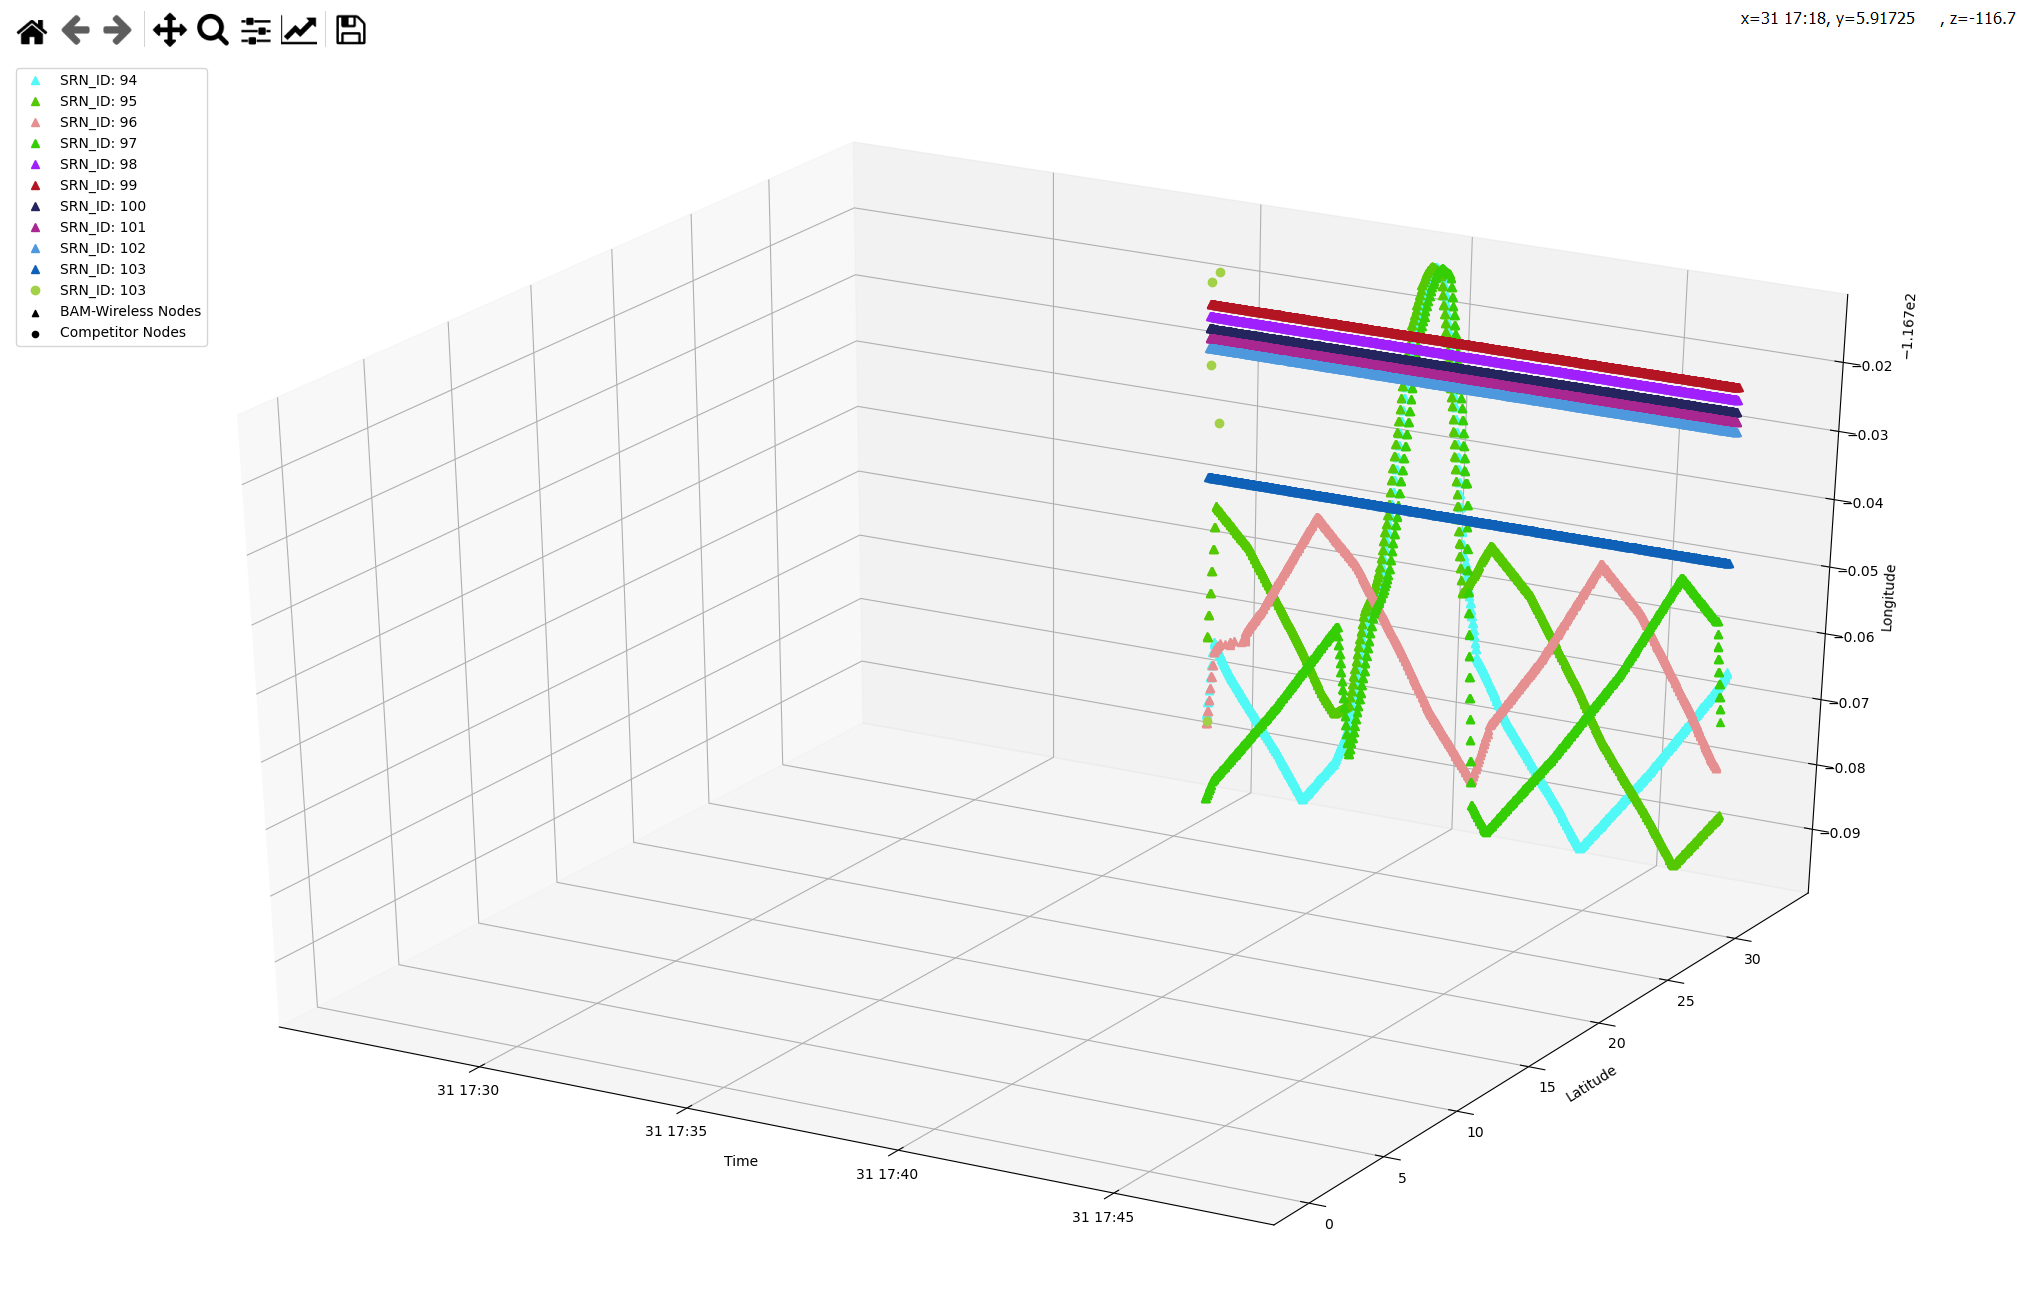
\includegraphics[width = 1.0\textwidth]{Wildfire_GPS.PNG}}
    \caption{The reported GPS locations of our SRNs, in addition to those of our competing SRNs, during the Wildfire scenario emulation}
    \label{fig:B.19}
\end{figure}
\begin{figure} [htb]
    \centerline{
    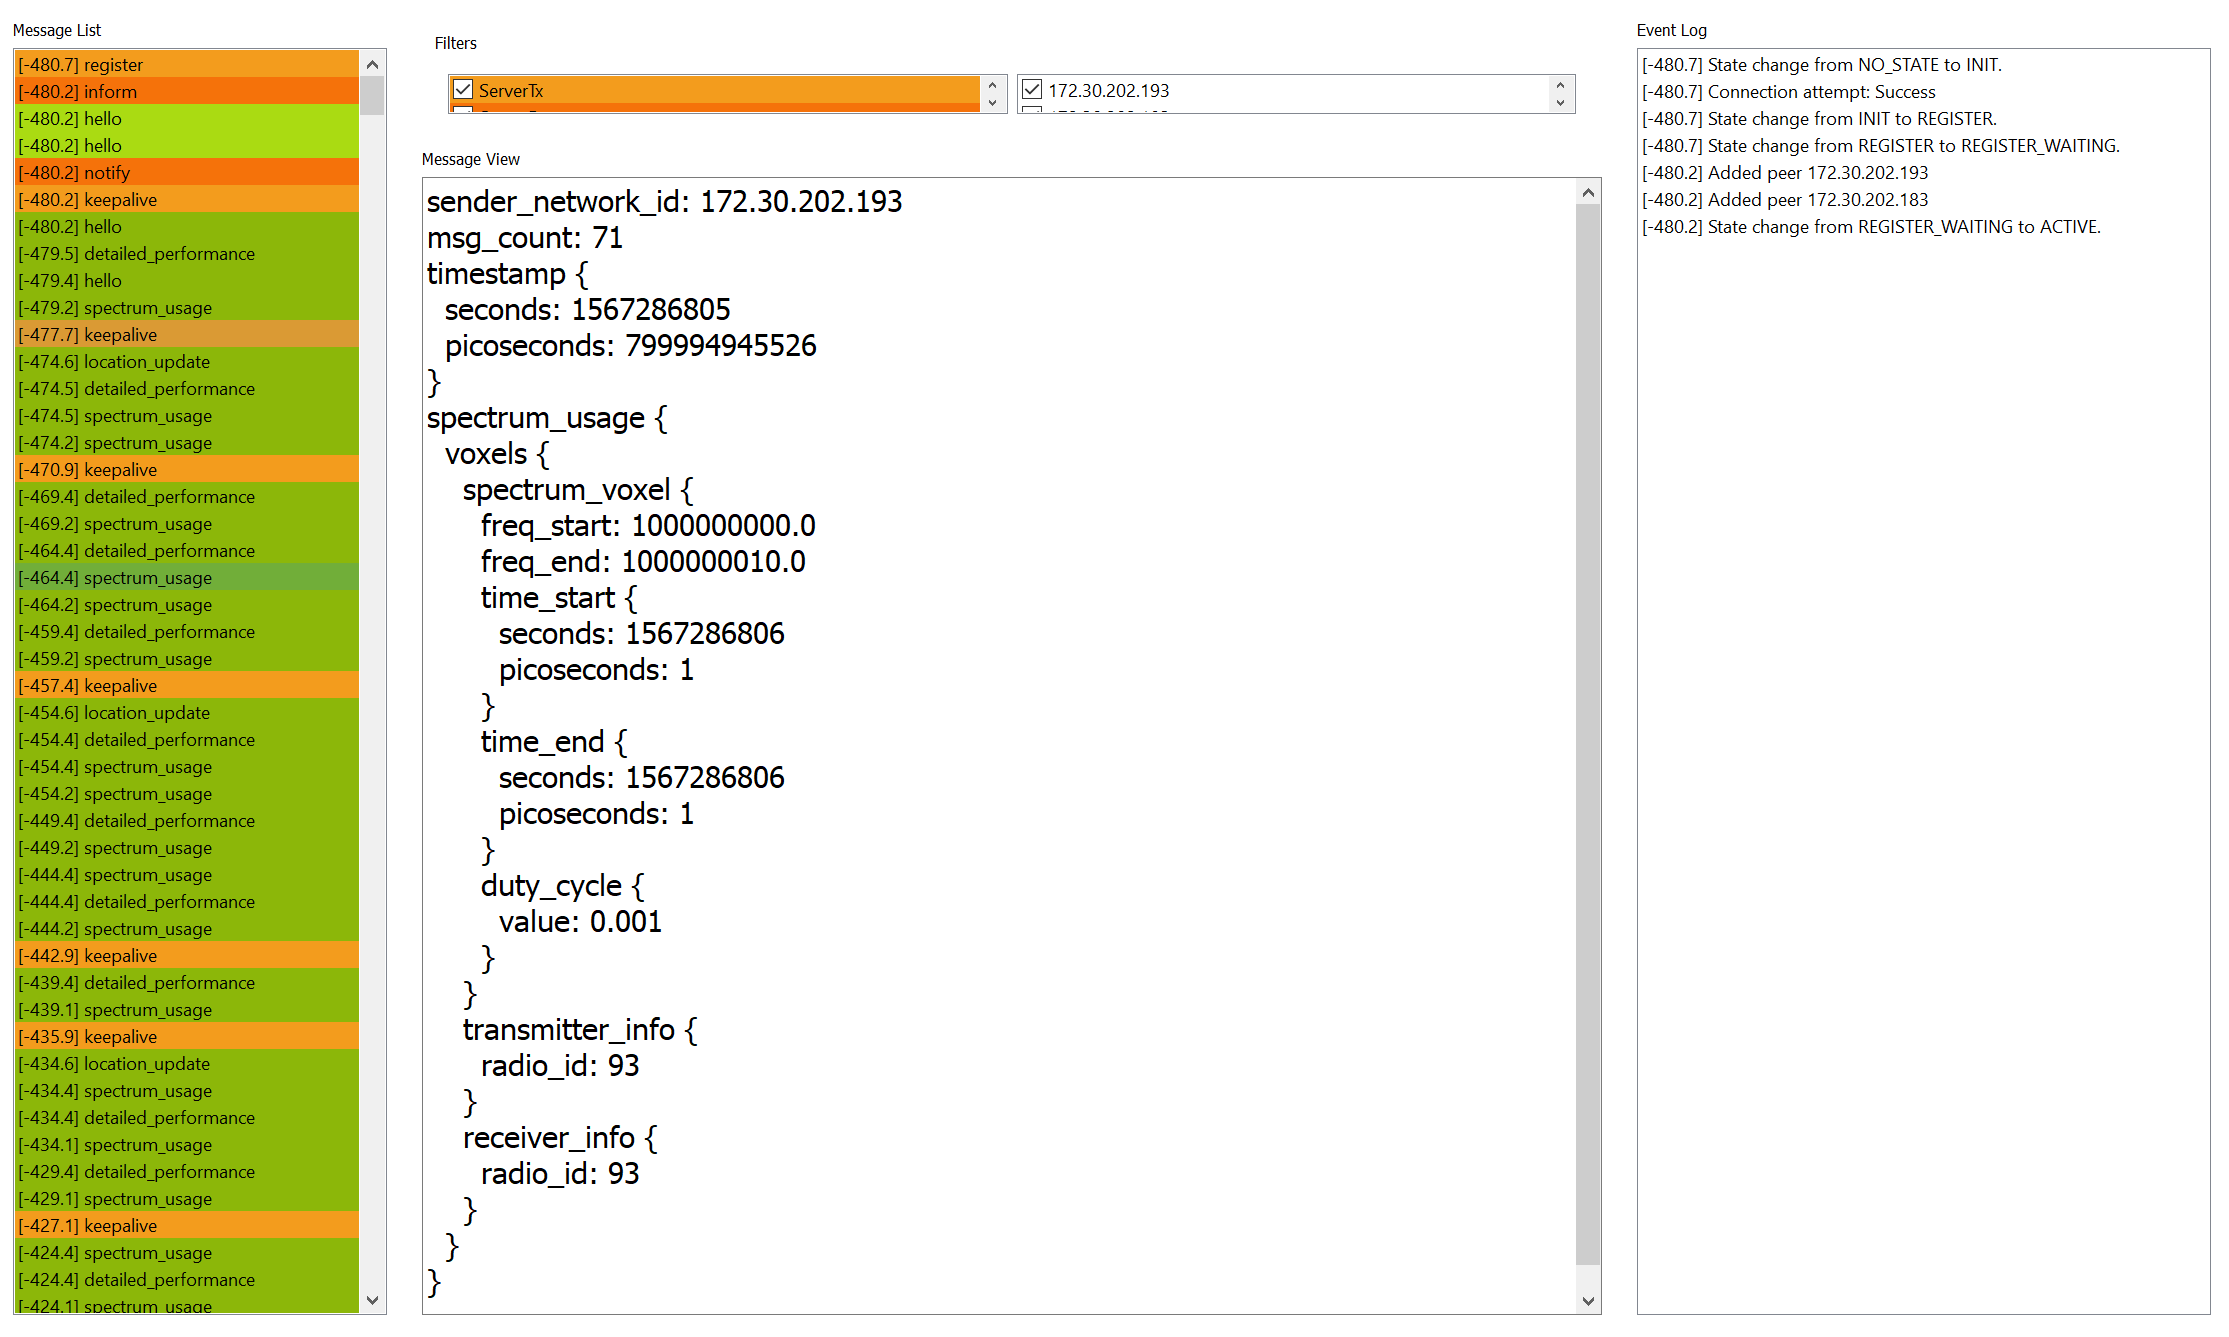
\includegraphics[width = 0.8\textwidth]{Wildfire_Collab.PNG}}
    \caption{The description of various CIL message exchanges between our network and the collaboration server, in addition to those between our network and our peers, during the Wildfire scenario emulation}
    \label{fig:B.20}
\end{figure}
\begin{figure} [htb]
    \centerline{
    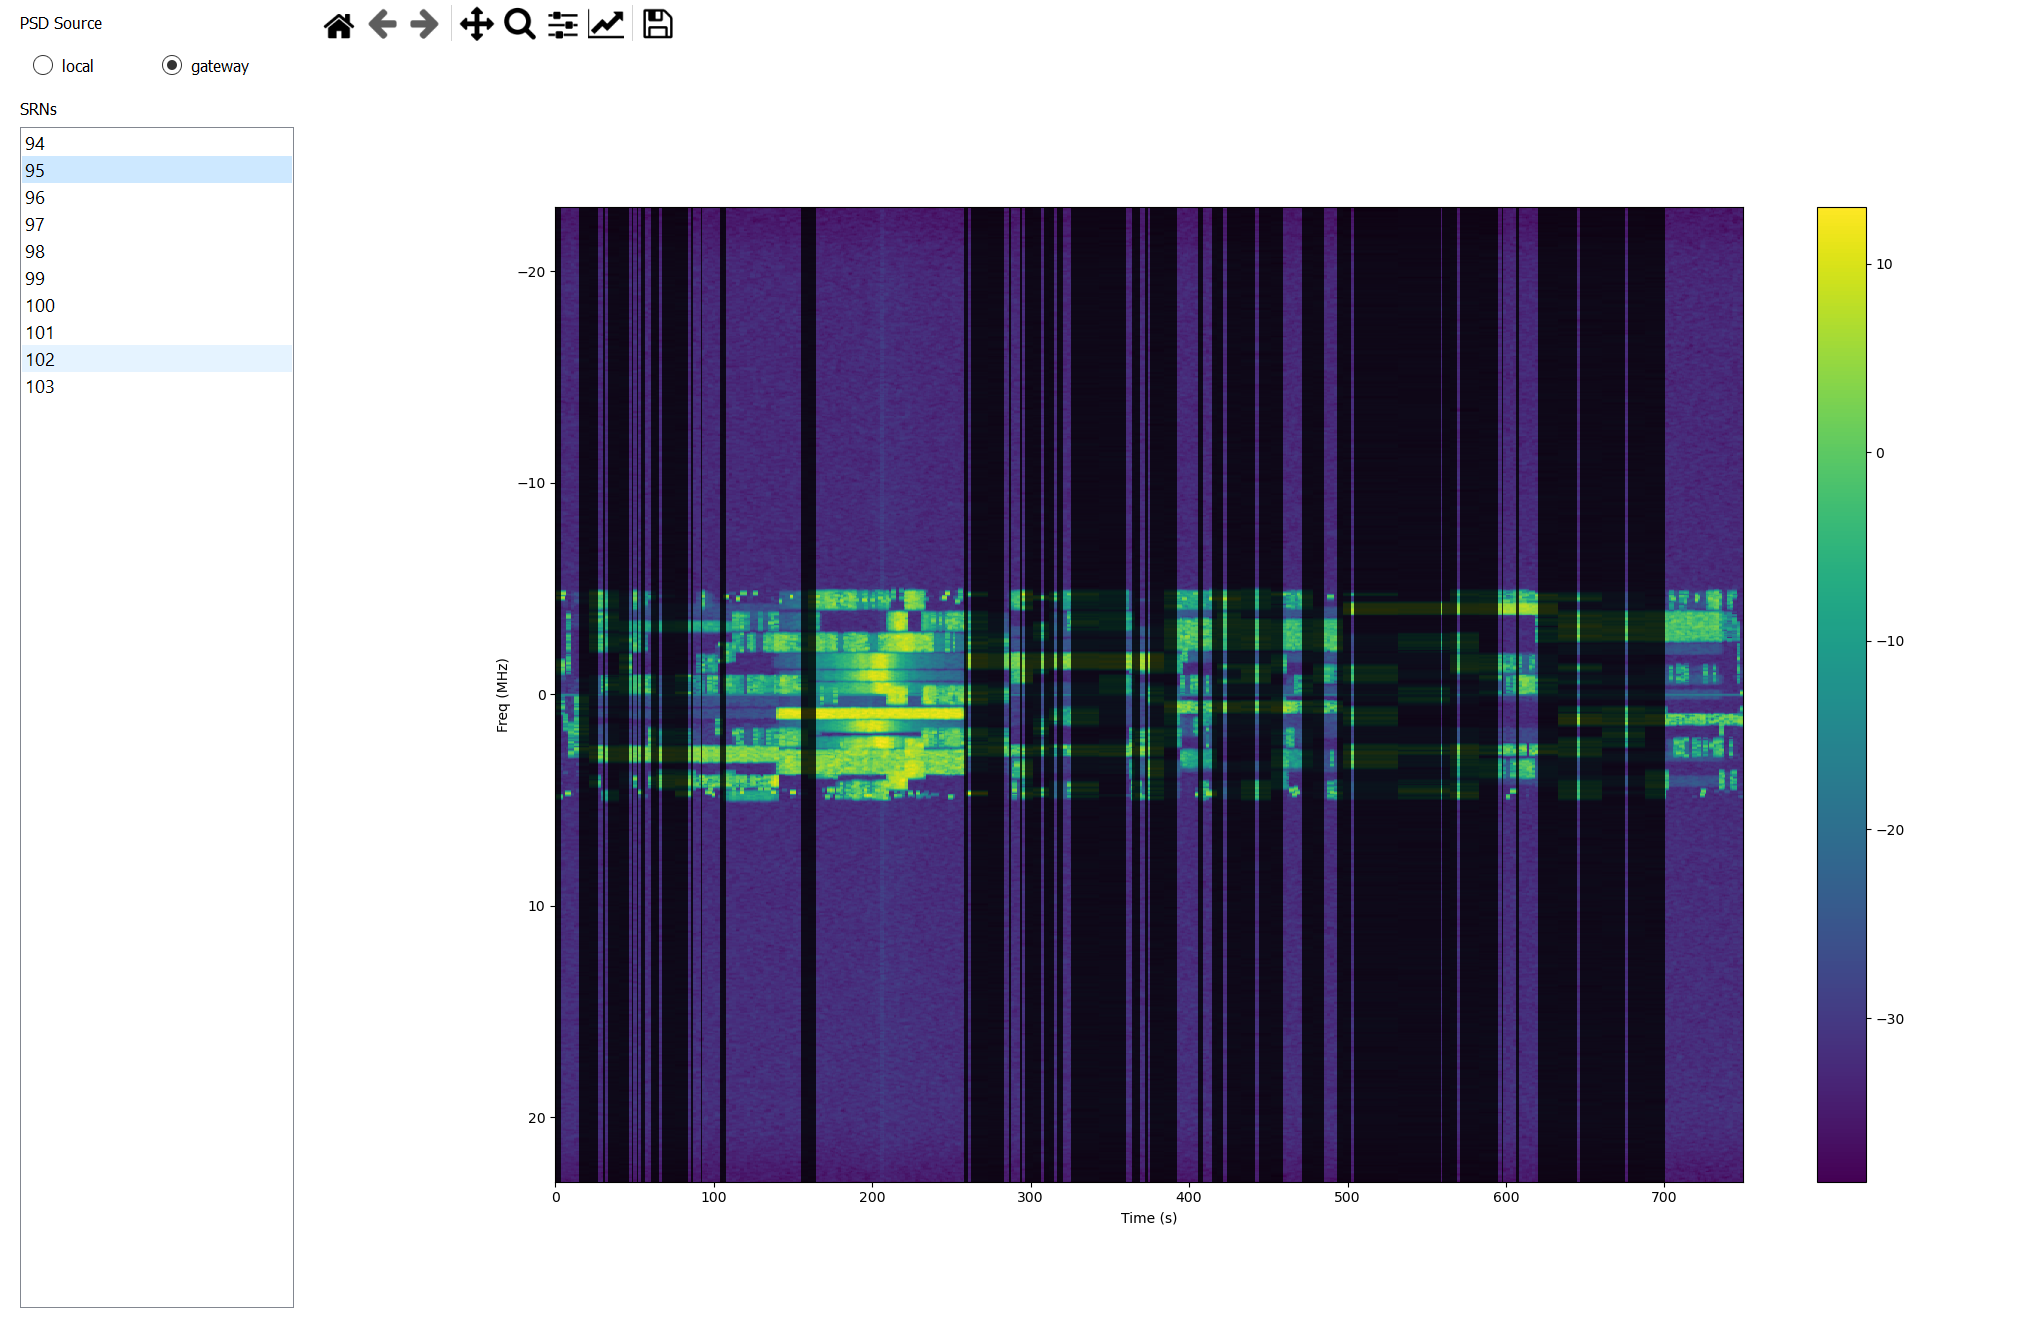
\includegraphics[width = 0.8\textwidth]{Wildfire_PSD.PNG}}
    \caption{The PSD measurements received at our Gateway SRN from one particular SRN in our network (selected), in order to obtain location-specific spectrum occupancy information, during the Wildfire scenario emulation}
    \label{fig:B.21}
\end{figure}

The reported GPS locations (latitude, longitude) of the SRNs in our CIRN, and the SRNs in our competitors' CIRNs, over time, are depicted in a $3$-dimensional time plot shown in Fig. \ref{fig:B.19}. The location information of these SRNs\texttt{-{}-}particularly, in relation to physical obstacles (emulated) and competitor SRNs, is employed in the channel allocation algorithm in our Gateway SRN. Fig. \ref{fig:B.20} illustrates the various timestamped CIL messages (both Client-Server messages and Peer-to-Peer messages) received by our Gateway SRN over the collaboration network\texttt{-{}-}these messages are exploited by our Gateway SRN, which along with the collated location-specific PSD measurements: one such PSD measurement in a given time snapshot observed at SRN with ID\texttt{-}$95$ and sent to our Gateway, is depicted in Fig. \ref{fig:B.21}\texttt{-{}-}determines a channel allocation (center frequencies) that minimizes the total interference caused at our SRNs by our competitors. Consequently, from an overall scenario duration perspective, the channel allocations of our network are collated into one ``big-picture" illustration, shown in Fig. \ref{fig:B.22}\texttt{-{}-}it is evident from this figure (the plot and the table underneath it) that the channel and bandwidth allocation strategy of our network is pretty consistent and stable throughout the scenario emulation.
\begin{figure} [htb]
    \centerline{
    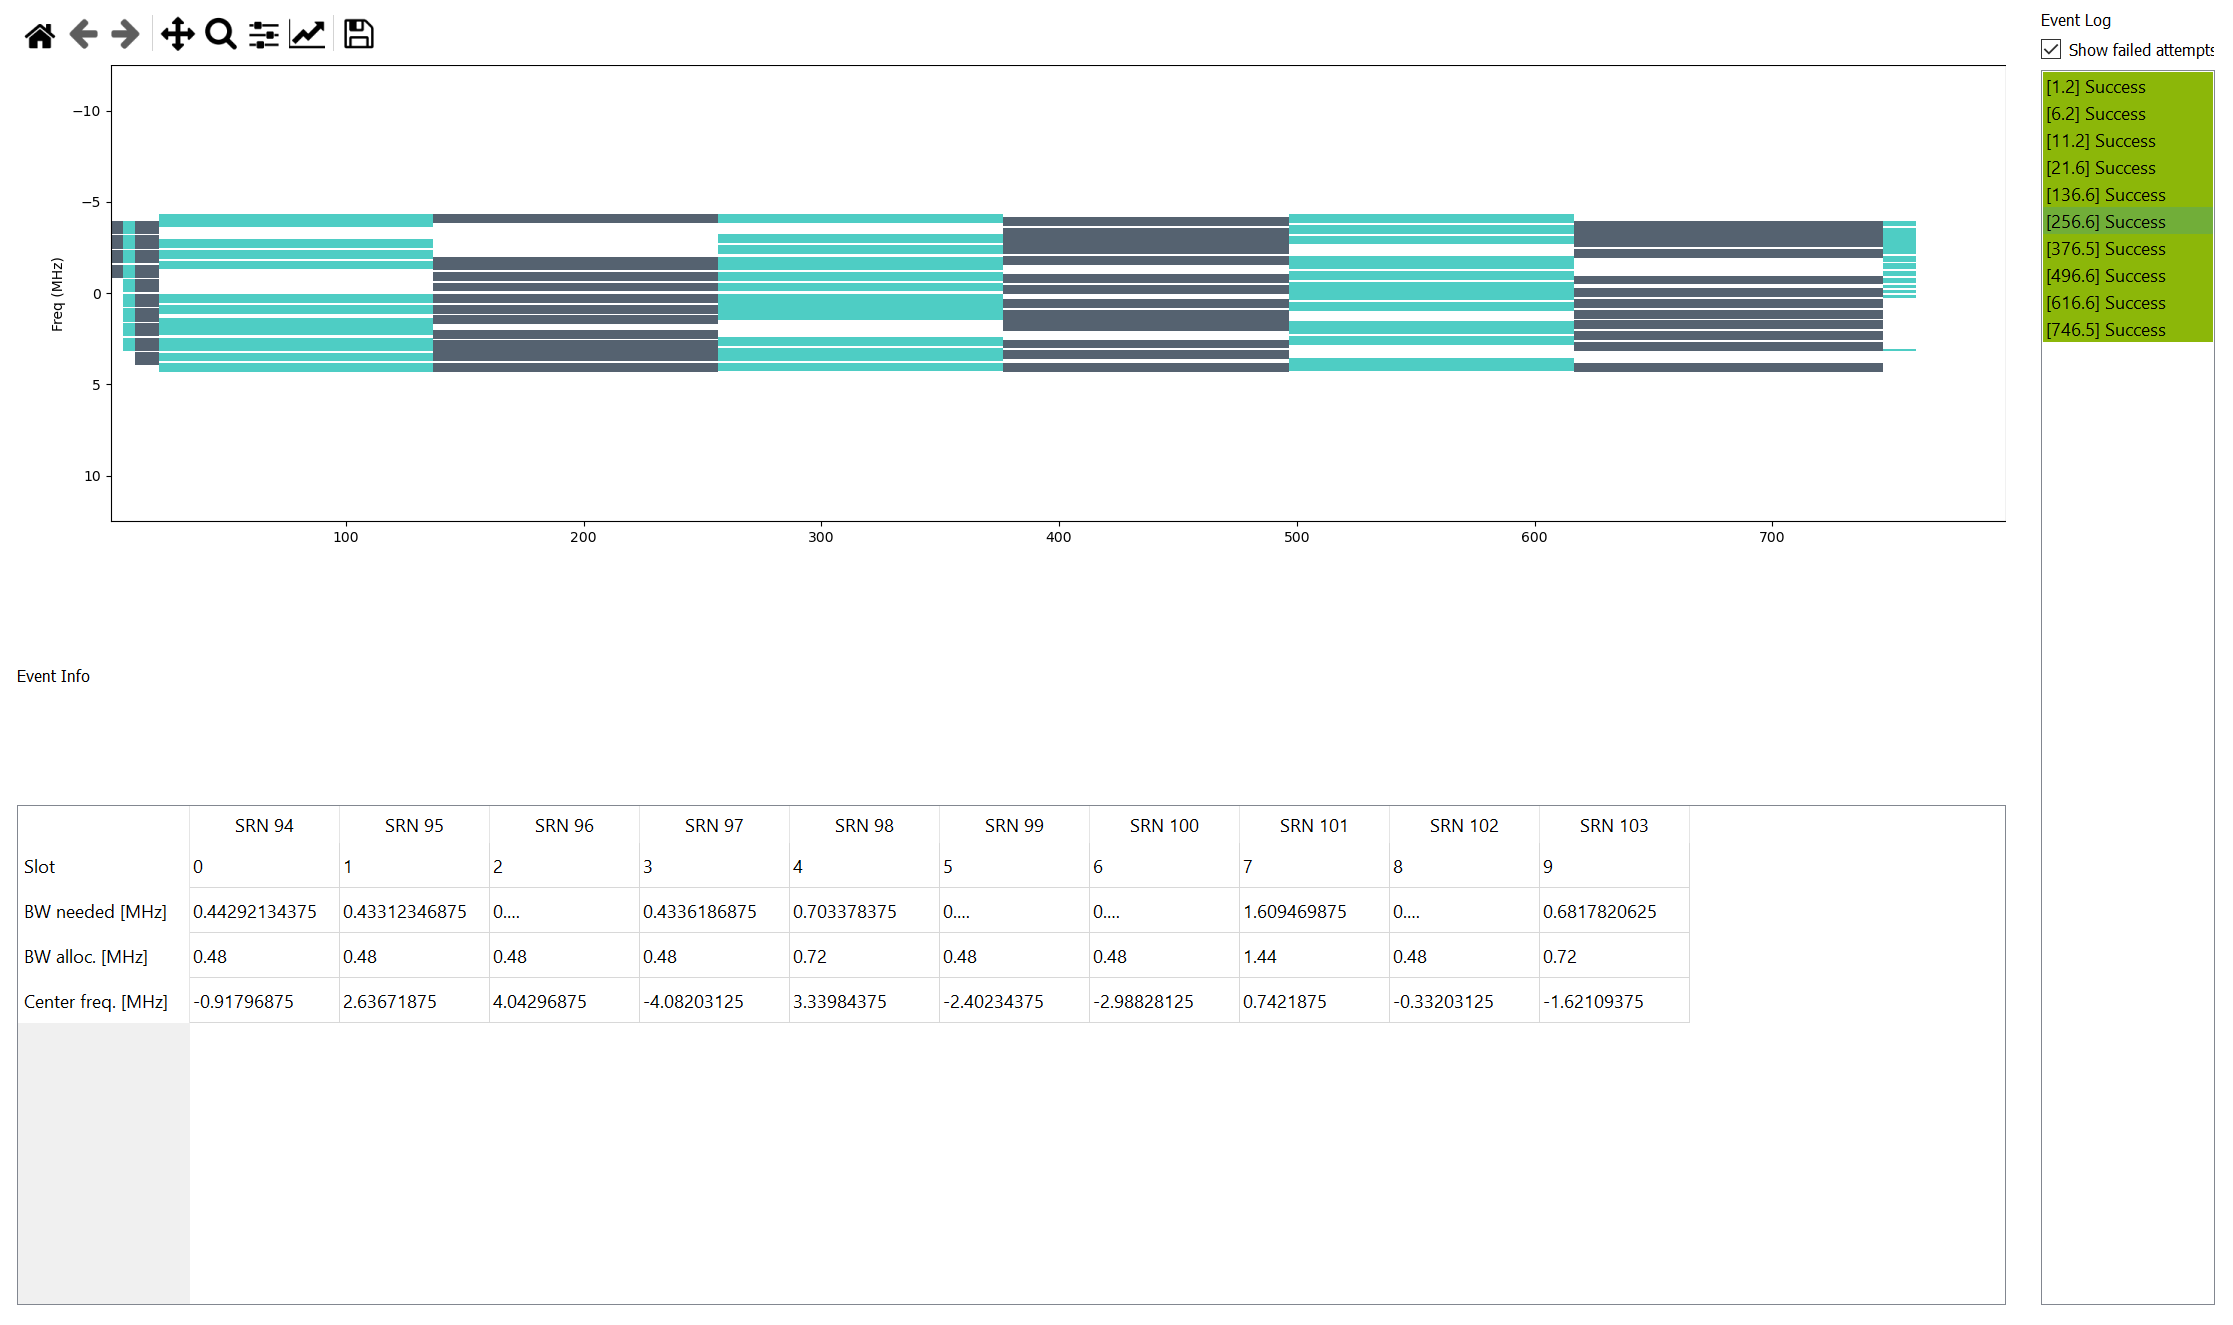
\includegraphics[width = 1.0\textwidth]{Wildfire_Channel_Alloc.PNG}}
    \caption{The spectrum occupancy behavior of SRNs in our network (as guided by our Gateway SRN) during the Wildfire scenario emulation}
    \label{fig:B.22}
\end{figure}
\section{Conclusion}\label{B.V}
In this chapter, we discussed the design principles of our cognitive radio developed for the DARPA SC2 Grand Challenge\texttt{-{}-}the transmission power control algorithm in the PHY for incumbent protection, the robust FSK control channel design, the high data rate DFT spread OFDM link for data traffic and ``long" control messages, the MCS adaptation algorithm in the PHY, the prioritized value-per-resource flow scheduling heuristic in the DLL with recursive revisitation, the channel and bandwidth allocation heuristic in the MAC, and the Dijkstra algorithm based multi-hop routing heuristic in the NET; the Radio Command and Control API (C2API) of the Colosseum that facilitates network management and orchestration; and the CIRN Interface Language (CIL) specifications, along with details about the collaboration network. Additionally, we presented component-wise plots illustrating the operational capabilities of our radios\texttt{-{}-}driven by the underlying design principles mentioned earlier, and evaluation of our network's performance against that of our competitors (other teams in this Grand Challenge: Northeastern University, Vanderbilt University, University of Florida, Virginia Tech (with Lockheed Martin), and Rutgers University, to name a few) in a military deployment scenario, i.e., Alleys of Austin, and a disaster-relief deployment scenario, i.e., Wildfire. Having presented the design of a cognitive radio node (and its deployment in a network of peers) and analyzed the operational capabilities and performance of our radios in quasi-collaborative scenario emulations, we now narrow our focus down to a specific problem\texttt{-{}-}the spectrum sensing and access problem in the MAC layer, and instead of proposing a complex heuristic like we did in this chapter, in the next chapter, we detail a highly rigorous approach to solve for the optimal spectrum sensing and access policy using an POMDP formulation.

\documentclass[10pt,twocolumn]{IEEEtran}
% \documentclass[12pt, draftcls, onecolumn]{IEEEtran}
\makeatletter
\def\subsubsection{\@startsection{subsubsection}
                                 {3}
                                 {\z@}
                                 {0ex plus 0.1ex minus 0.1ex}
                                 {0ex}
                             {\normalfont\normalsize\bfseries}}
\makeatother
\usepackage[T1]{fontenc}
\usepackage{subfigure}
\usepackage{ulem}
\usepackage{amsmath}
\allowdisplaybreaks
\usepackage{hhline}
\usepackage{graphicx}
\usepackage{yfonts,color}
\usepackage{soul,xcolor}
\usepackage{verbatim}
\usepackage{amsmath}
\allowdisplaybreaks
\usepackage{amssymb}
\usepackage{amsthm}
\usepackage{float}
\usepackage{bm}
\usepackage{url}
\usepackage{array}
\usepackage{cite}
\usepackage{tikz}
\usepackage{framed}
\usepackage{balance}
\usepackage{epsfig,epstopdf}
\usepackage{booktabs}
\usepackage{courier}
\usepackage{subfigure}
\usepackage{pseudocode}
\usepackage{enumerate}
\usepackage{algorithm}
\usepackage{algpseudocode}
\newtheorem{definition}{Definition}
\newtheorem{theorem}{Theorem}
\newtheorem{lemma}[theorem]{Lemma}
\newtheorem{proposition}[theorem]{Proposition}
\newtheorem{corollary}[theorem]{Corollary}
\newtheorem{assumption}{Assumption}
\newtheorem{remark}{Remark}
\renewcommand{\algorithmicrequire}{\textbf{Initialization:}}  
\renewcommand{\algorithmicensure}{\textbf{Output:}}  
\newcommand{\rom}[1]{\uppercase\expandafter{\romannumeral #1\relax}}
\usepackage{color}
\usepackage{soul,xcolor}
\newcommand{\sst}[1]{\st{#1}}
%\newcommand{\sst}[1]{}
\newcommand{\nm}[1]{{\color{blue}\bf{[NM: #1]}}}
%\newcommand{\nm}[1]{}
\newcommand{\bk}[1]{{\color{magenta}{[BK: #1]}}}
\newcommand{\nmmath}[1]{{\color{blue}\text{\bf{[NM: #1]}}}}
\newcommand{\gs}[1]{{\color{orange}\bf{[GS: #1]}}}
\newcommand{\remove}[1]{{\color{magenta}{\bf REMOVE: [#1]}}}
\DeclareMathOperator*{\argmax}{arg\,max}
\DeclareMathOperator*{\argmin}{arg\,min}
\usepackage{cancel}
\newcommand\mst[2][red]{\setbox0=\hbox{$#2$}\rlap{\raisebox{.45\ht0}{\textcolor{#1}{\rule{\wd0}{2pt}}}}#2} 
%\newcommand\mst[2][red]{} 
\newcommand{\add}[1]{{\color{red}{#1}}}
\newcommand{\ull}[1]{\textbf{\color{red}\ul{#1}}}
\renewcommand{\baselinestretch}{0.96}
\normalem
\title{Spectrum Sensing in Cognitive Radio Networks
\\
via Approximate POMDP}
\author{Bharath Keshavamurthy, Nicol\`{o} Michelusi
\thanks{This research has been funded in part by NSF under grant CNS-1642982.}
\thanks{The authors are with the School of Electrical and Computer Engineering, Purdue University. email: \{bkeshava,michelus\}@purdue.edu.}
\vspace{-12mm}}
\begin{document}
\maketitle
\thispagestyle{empty}
\pagestyle{empty} 
\setulcolor{red}
\setul{red}{2pt}
\setstcolor{red}
\begin{abstract}
In this paper, a novel spectrum sensing and access strategy based on POMDPs is proposed. A cognitive radio learns the correlation models defining the occupancy behavior of incumbents, based on which it devises an optimal spectrum sensing and access policy. The optimization complexity is ameliorated via point-based value iteration methods. Numerical evaluations demonstrate that our framework achieves higher SU throughput with lower PU interference, compared to clustering algorithms from the state-of-the-art and a Neyman-Pearson detector that assumes independence among channels. Furthermore, our scheme achieves the throughput and interference levels attained by HMM MAP estimators that possess these correlation models apriori.
\end{abstract}
\begin{IEEEkeywords}
Hidden Markov Model, Cognitive Radio, Spectrum Sensing, POMDP
\end{IEEEkeywords}
\vspace{-5mm}
\section{Introduction}\label{I}
The advent of fifth-generation wireless communication networks has exacerbated the problem of spectrum scarcity \cite{7158089}. Cognitive radio networks facilitate efficient spectrum utilization by intelligently accessing \emph{white spaces} left unused by the sparse and infrequent transmissions of licensed users, while ensuring rigorous incumbent non-interference compliance \cite{4562537}. 

A crucial aspect underlying the design of cognitive radio networks is the ability to perform spectrum sensing. However, physical design limitations are imposed on the cognitive radio's spectrum sensor in view of quick turnaround times and energy efficiency \cite{5990482}, which restrict the number of channels that can be sensed at any given time. This has led to research in algorithms that first determine the best channels to sense, after which the gathered information is used to perform channel access. The state-of-the-art are based on multi-armed bandits \cite{7094730}, reinforcement learning \cite{6507570}, and custom heuristics \cite{4554696, 6956794}. However, most of these works, such as \cite{7094730, 6507570, 7895211, 7336513, 8571293}, assume independence across frequency bands, which is imprudent because licensed users may exhibit correlation across both frequency and time in their channel occupancy behavior: they may occupy a set of adjacent frequency bands for an extended period of time \cite{6188346}. This correlation structure may be leveraged for more accurate predictions of spectrum holes. In this paper, we propose a parameter estimation algorithm to learn the frequency and time correlation structure, based on which we solve for the optimal sensing and access policy.

Distributed spectrum sensing has been considered in \cite{6507570} and solved using SARSA with linear value function approximation. However, frequency correlation is precluded, and errors in state estimation are neglected in the decision process. In \cite{6956794}, the frequency correlation is exploited, but a noise-free observation model is assumed. Compared to \cite{6507570, 6956794}, we account for the uncertainty in the occupancy state and for noisy observations via a partially observable Markov decision process (POMDP) formulation. Standard MAP-based state estimators for Hidden Markov Models (HMMs) such as the Viterbi algorithm can be employed to estimate spectrum occupancy \cite{4554696}; however, these estimators rely on knowledge of the transition model, which may be unknown in practice. Therefore, in our paper, we embed a parameter estimation algorithm to learn the parametric time-frequency correlation models. Additionally, \cite{4554696} does not impose sensing restrictions on the cognitive radio. Finally, in \cite{6956794, 4554696}, the time-frequency correlation structure is estimated offline based on pre-loaded databases. Instead, in our work, we present a fully online framework to estimate it, and simultaneously, solve for the optimal sensing and access policy.

The contributions of this paper are as follows: a POMDP formulation detailing the optimization problem for spectrum sensing and access in a radio environment with multiple licensed users exhibiting correlations in their occupancy behavior across both time and frequency, assuming a linear, Gaussian observation model with sensing limitations; an online parameter estimation algorithm to learn these correlation models; and a concurrent randomised point-based value iteration algorithm that solves the POMDP formulation for the optimal spectrum sensing and access policy. The rest of the paper is organized as follows: in Sec. \ref{II}, we define the system model, followed by the formulations, approaches, and algorithms in Sec. \ref{III}; in Sec. \ref{IV}, we present numerical evaluations, followed by our conclusions in Sec. \ref{V}.
\vspace{-4mm}
\section{System Model}\label{II}
\noindent {\bf Signal Model:}
We consider a network consisting of $J$ licensed users termed the Primary Users (PUs) and one cognitive radio termed the Secondary User (SU) equipped with a spectrum sensor. The objective of the SU is to opportunistically access portions of the spectrum left unused by the PUs in order to maximize its own throughput. To this end, the SU should learn how to intelligently access spectrum holes (white spaces) intending to maximize its throughput while maintaining strict non-interference compliance with incumbent transmissions. The observed wideband signal in the frequency domain is given by
\begin{equation}\label{2}
    Y_k(i) = \sum_{j=1}^{J} H_{j,k}(i)X_{j,k}(i) + V_k(i),
\end{equation}
where $i {\in} \{1,2,3,\dots,T\}$ represents the time index; $k {\in} \{1,2,3,\dots,K\}$ represents the index of the components in the frequency domain; $V_k(i) {\sim} \mathcal{CN}(0,\sigma_V^2)$ represents circularly symmetric additive complex Gaussian noise, i.i.d across frequency and across time, and independent of $H$ and $X$; $X_{j,k}(i)$ is the signal of the $j$th PU in the frequency domain, and $H_{j,k}(i)$ is its frequency domain channel. We further assume that the $J$ PUs employ an orthogonal access to the spectrum (e.g., OFDMA) so that $X_{j,k}(i)X_{g,k}(i)=0, \forall j{\neq}g$. Thus, letting $j_{k}$ be the index of the PU that contributes to the signal in the $k$th spectrum band, and letting  $H_{k}(i){=}H_{j_{k},k}(i)$ and $X_{k}(i){=}X_{j_{k},k}(i)$ (with $X_{k}(i){=}0$ if no PU is transmitting in the $k$th spectrum band at time $i$), we can rewrite \eqref{2} as 
\begin{equation}\label{3}
    Y_k(i) = H_{k}(i)X_{k}(i) + V_k(i).
\end{equation}
We model $H_{k}(i)$ as a zero-mean circularly symmetric complex Gaussian random variable with variance $\sigma_H^2$, $H_k {\sim} \mathcal{CN}(0,\sigma_H^2)$, i.i.d. across frequency bands, over time, and independent of the occupancy state of the channels.
\begin{figure}
    \centering
    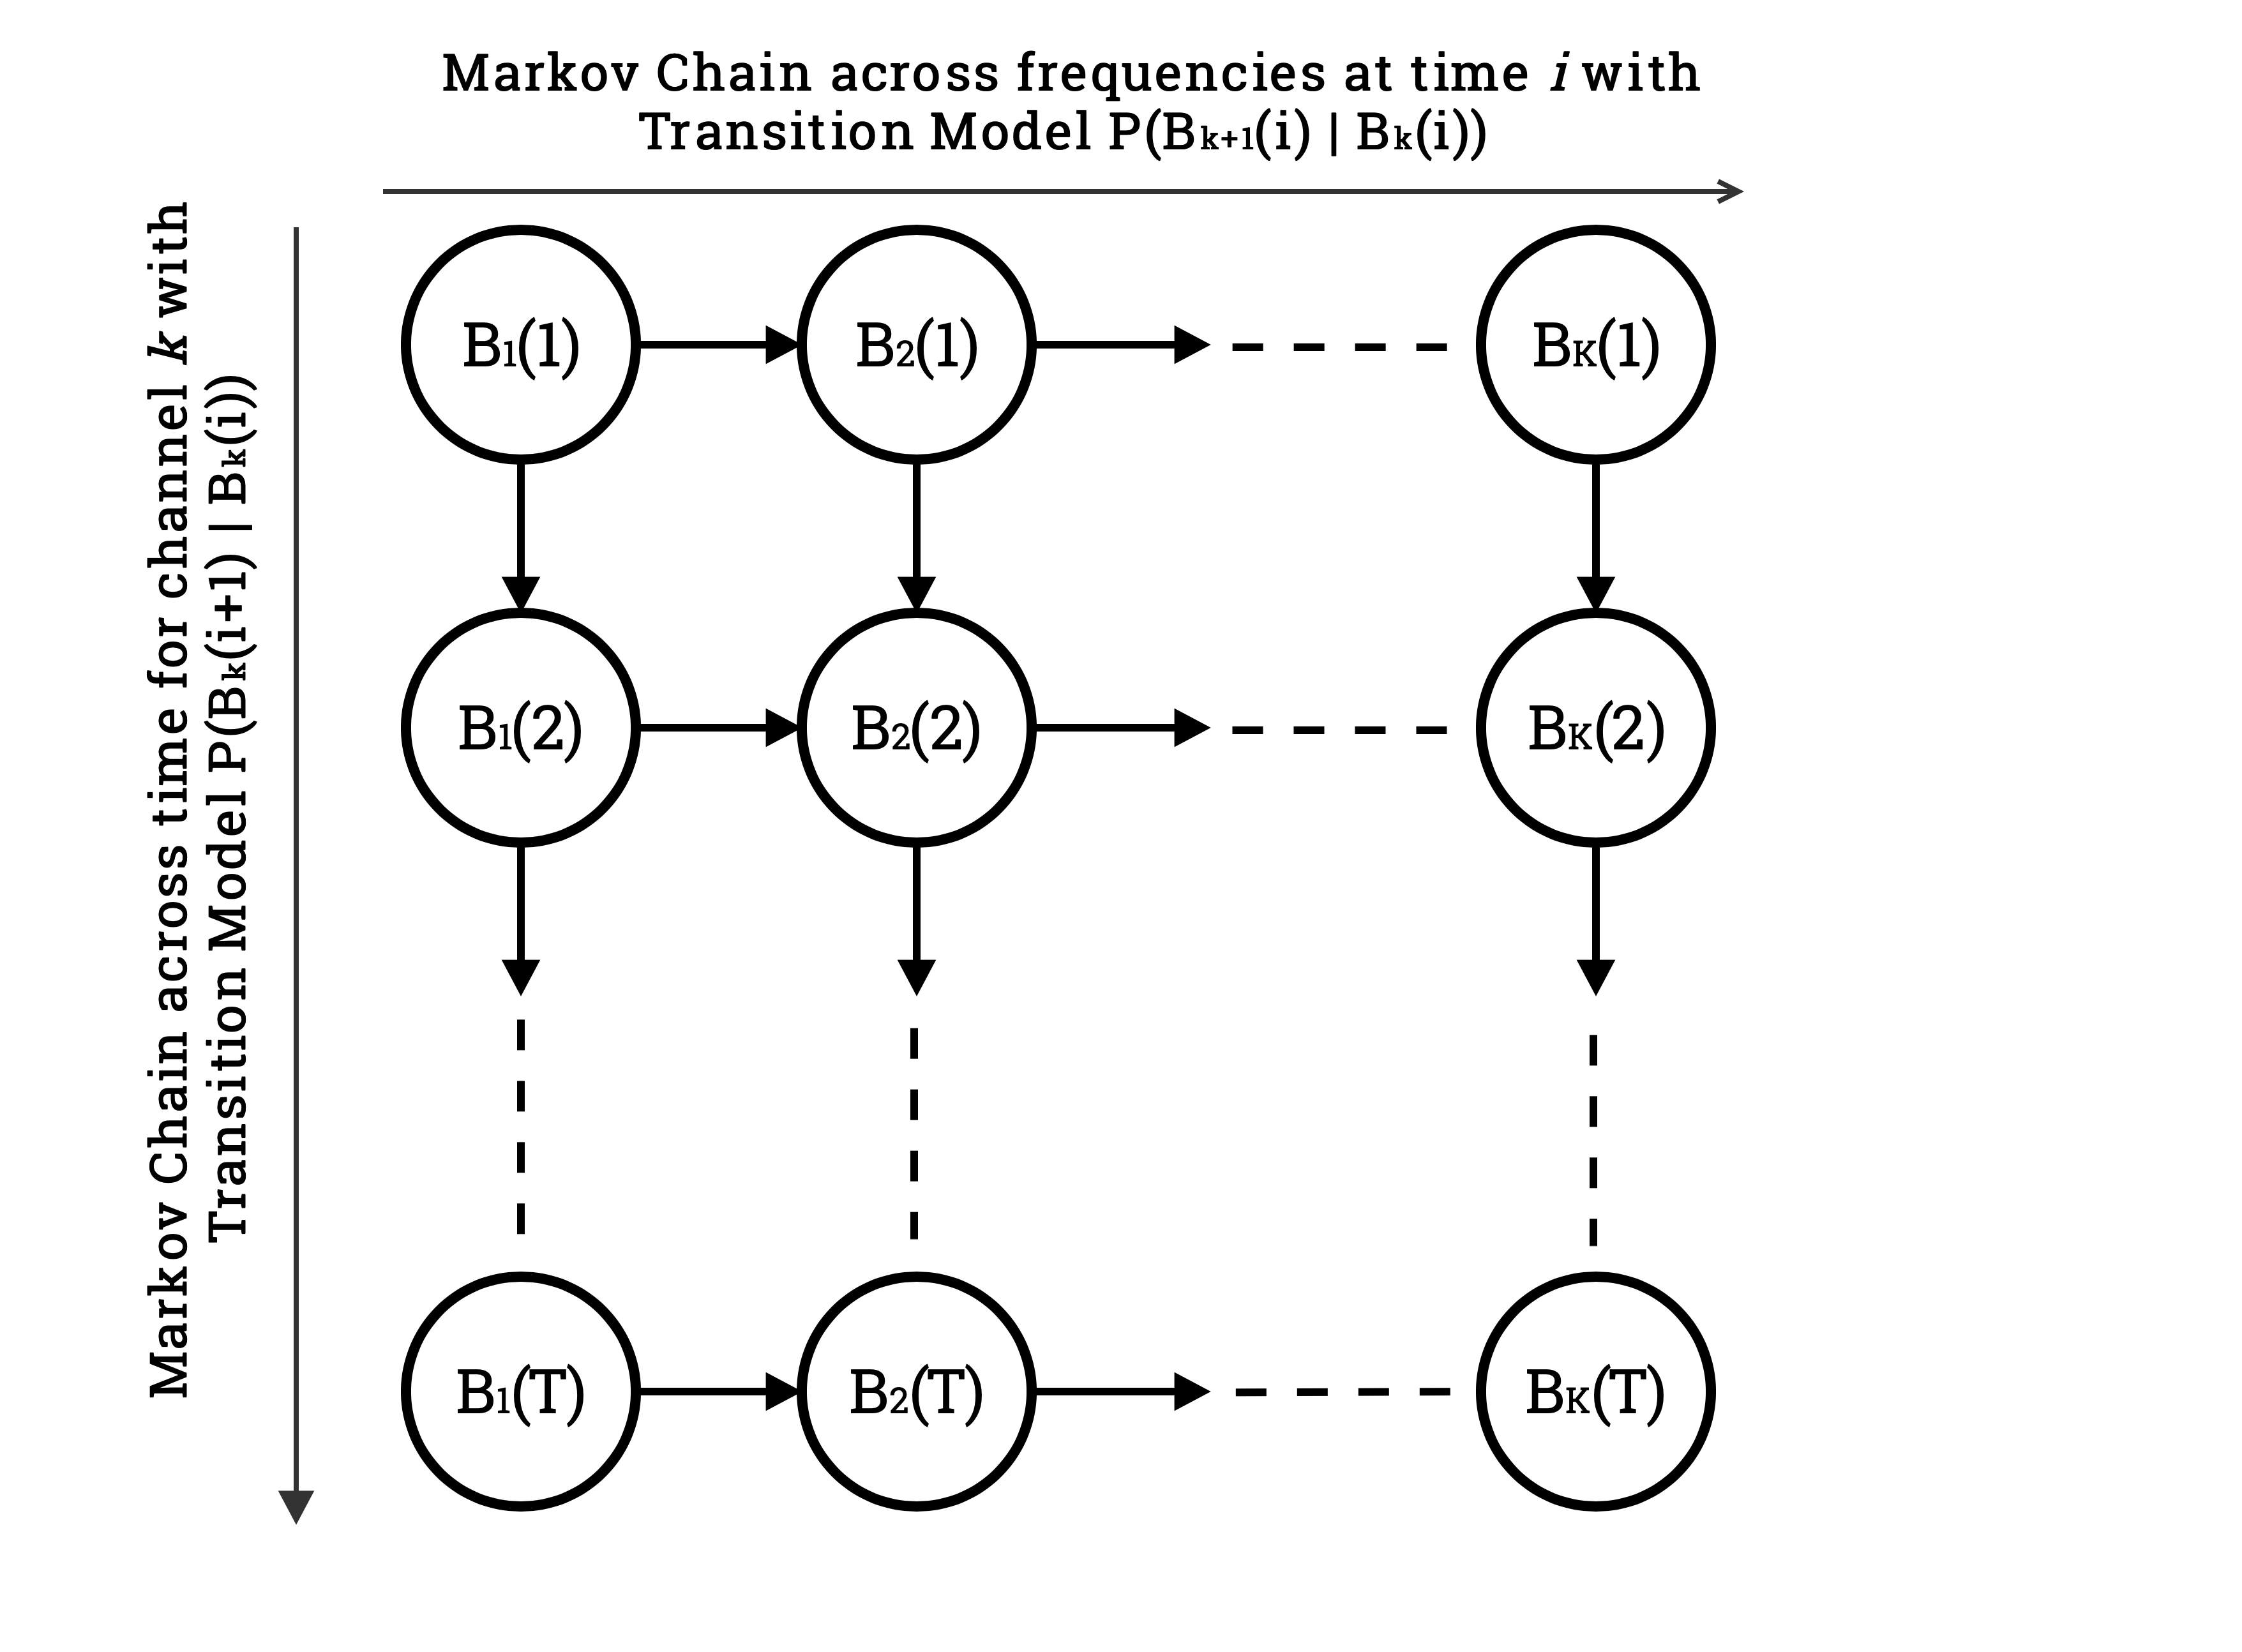
\includegraphics[width=0.80\linewidth]{MarkovChainsVisualization}
    \vspace{-5mm}
    \caption{The correlation model across time and frequencies underlying the occupancy behavior of incumbents in the network}
    \vspace{-5mm}
    \label{fig:1}
\end{figure}
%\vspace{-3mm}

\noindent {\bf PU Spectrum Occupancy Model:}
We now introduce the model of PU occupancy over time and across the frequency domain. We model each $X_k(i)$ as 
\begin{equation}\label{4}
    X_k(i) = \sqrt{P_{tx}}B_k(i)S_k(i),
\end{equation}
where $P_{tx}$ is the transmission power of the PUs, $S_k(i)$ is the transmitted symbol modelled as a constant amplitude signal, $|S_k(i)|{=}1$, i.i.d. over time and across frequency bands;\footnote{In the case where $S_k(i)$ does not have constant amplitude, we may approximate $H_{k}(i)S_{k}(i)$ as complex Gaussian with zero mean and variance $\sigma_H^2\mathbb E[|S_{k}(i)|^2]$, without any modification to the subsequent analysis.} $B_k(i){\in}\{0,1\}$ is the binary spectrum occupancy variable, with $B_k(i){=}1$ if the $k$th spectrum band is occupied by a PU at time $i$, and $B_k(i){=}0$ otherwise. Therefore, the PU occupancy behavior in the entire wideband spectrum of interest at time $i$, discretized into narrow-band frequency components can be modeled as the vector 
\begin{equation}\label{5}
    \vec{B}(i) = [B_1(i), B_2(i), B_3(i), \cdots, B_K(i)]^T {\in} \{0, 1\}^K.
\end{equation}
PUs join and leave the spectrum at random times. To capture this temporal correlation in the spectrum occupancy dynamics of PUs, we model $\vec{B}(i)$ as a Markov process,
\begin{equation}\label{6}
    \begin{aligned}
        \mathbb{P}(\vec{B}(i+1)|\vec{B}(j), \forall j \leq i) = \mathbb{P}(\vec{B}(i+1)|\vec{B}(i)).
    \end{aligned}
\end{equation}
Additionally, when joining the spectrum pool, PUs occupy a number of adjacent spectrum bands, and may vary their spectrum needs depending on traffic demands, channel conditions, etc. To capture this behavior, we model $\vec{B}(i)$ as having Markovian correlation across spectrum bands,
\begin{align}\label{7}
&         \mathbb{P}(\vec{B}(i+1)|\vec{B}(i))\\&=
\nonumber
         \mathbb{P}(B_{1}(i+1)|B_{1}(i))
         \prod_{k=2}^{K} \mathbb{P}(B_{k}(i+1)|B_{k}(i), B_{k-1}(i+1)).
\end{align}
That is, the spectrum occupancy at time $i+1$ in frequency band $k$, $B_{k}(i+1)$, depends on the  occupancy state of the adjacent spectrum band at the same time, $B_{k-1}(i+1)$, and that of the same spectrum band $k$ in the previous time index $i$, $B_{k}(i)$ as shown in Fig. \ref{fig:1}. We structure the correlation models as two Markov chains: one across time and the other across frequencies, where the chain across frequencies is parameterized by $p{=}\mathbb{P}(B_{k}(i+1){=}1|B_{k-1}(i+1){=}0)$ and the chain across time is parameterized by $q{=}\mathbb{P}(B_{k}(i+1){=}1|B_{k}(i){=}0)$. We estimate these parameters $p$ and $q$, parameterizing each of these two chains, using the parameter estimation algorithm described in Sec. \ref{III} in order to obtain the transition model underlying the MDP, given by \eqref{7}.
% \vspace{-3mm}

\noindent{\bf Spectrum Sensing Model:}
In order to detect the available spectrum holes, the SU performs spectrum sensing. However, owing to physical design limitations at the SU's spectrum sensor, the SU can sense only $\kappa$ out of $K$ spectrum bands at any given time, with $1{\leq}\kappa{\leq}K$. Let $\mathcal K_{i}{\subseteq}\{1,2,\dots,K\}$ with $|\mathcal K_i|{\leq}\kappa$ be the set of indices of spectrum bands sensed by the SU at time $i$, which is part of our design.
Then, we define the observation vector
\begin{equation}\label{8}
    \vec{Y}(i) = [Y_k(i)]_{k {\in} \mathcal K_i},
\end{equation}
where $Y_k(i)$ is given by \eqref{3}.
The true states $\vec{B}(i)$ encapsulate the actual occupancy behavior of the PU and the measurements at the SU are noisy observations of these true states which are modeled to be the observed states of an HMM. Given $\vec{B}(i)$ and $\mathcal K_i$, the probability density function of $\vec{Y}(i)$ is
\begin{equation}\label{9}
    f(\vec{Y}(i)|\vec{B}(i), \mathcal K_i) = \prod_{k \in \mathcal K_i} f(Y_k(i)|B_k(i)),
\end{equation}
owing to the independence of channels (given the occupancy states), noise, and transmitted symbols across frequency bands. Moreover, from \eqref{3},
\begin{equation}\label{10}
 Y_k(i)|B_k(i) \sim \mathcal{CN}(0, \sigma_H^2P_{tx}B_k(i) + \sigma_V^2).
\end{equation}

\noindent{\bf POMDP Agent Model:}
In this section, we model the spectrum access scheme of the SU as a POMDP, whose goal is to devise an optimal sensing and access policy in order to maximize its throughput while maintaining strict non-interference compliance with incumbent transmissions. In fact, the agent's limited sensing capabilities coupled with its noisy observations result in an increased level of uncertainty at the agent's end about the occupancy state of the spectrum under consideration and the exact effect of executing an action on the radio environment. The transition model of the underlying MDP as described by \eqref{7}, is denoted by $\mathbf{A}$ and is learned by the agent by interacting with the radio environment (see Sec. \ref{III}). The emission model is denoted by $\mathbf{M}$ and is given by \eqref{9}, with $f(Y_k(i)|B_k(i))$ given by \eqref{10}. 

We model the POMDP as a tuple $(\mathcal B,\mathcal{A},\mathcal{Y},\mathbf{A},\mathbf{M})$ where $\mathcal{B}\equiv\{0,1\}^K$ represents the state space of the underlying MDP with states $\vec{B}$, given by all possible realizations of the spectrum occupancy vector as described by \eqref{5}; $\mathcal{A}$ represents the action space of the agent, given by all possible combinations in which $\kappa$ spectrum bands are chosen to be sensed out of $K$ at any given time; and $\mathcal{Y}$ represents the observation space of the agent based on the aforementioned signal model. The state of the POMDP at time $i$ is given by the \emph{prior belief} $\beta_i$, which represents the probability distribution of the underlying MDP state $\vec{B}(i)$, given the information collected by the agent up to time $i$, but before collecting the new information in time-step $i$. At the beginning of each time index $i$, given $\beta_i$, the agent selects $\kappa$ spectrum bands out of $K$, according to a policy $\pi(\beta_i)$, thus defining the sensing set $\mathcal K_i$, performs spectrum sensing  on these spectrum bands, observes $\vec{Y}(i){\in} \mathcal{Y}$, and updates its \emph{posterior belief} $\hat{\beta}_i$ of the current spectrum occupancy $\vec{B}(i)$ as 
\begin{align}\label{11}
\hat\beta_i(\vec{B}') &= \mathbb{P}(\vec{B}(i) = \vec{B}'|\vec{Y}(i), \mathcal K_i, \beta_i)\\&=
\nonumber
\frac{\mathbb{P}(\vec{Y}(i)|\vec{B}', \mathcal{K}_i) \beta_i(\vec{B}')}{
\sum_{\vec{B}'' {\in} \{0,1\}^K} \mathbb{P}(\vec{Y}(i)|\vec{B}'', \mathcal{K}_i) \beta_i(\vec{B}'')}.
\end{align}
We denote the function that maps the prior belief $\beta_i$ to the posterior belief $\hat\beta_i$ through the spectrum sensing action $\mathcal K_i$ and the observation signal $\vec{Y}(i)$ as $\hat\beta_i{=}\hat{\mathbb B}(\beta_i, \mathcal K_i, \vec{Y}(i))$.

Given the posterior belief $\hat{\beta}_i$, we estimate the occupancy state of the discretized spectrum under consideration as $\vec{B}(i)^{*}{=}\argmax_{\vec{B} {\in} \mathcal{B}} \hat{\beta}_{i}(\vec{B})$. Let $B_{k}(i)^{*}{=}\phi_{k}(\hat{\beta}_{i}) {\in} \{0, 1\}$ be the estimated state of channel $k$ at time $i$. If the channel is deemed to be idle as a result of this MAP estimation procedure, i.e., $\phi_{k}(\hat{\beta}_{i}){=}0$, the SU accesses the channel for delivering its network flows. Else, it leaves it untouched. Given the PU occupancy state $\vec{B}(i)$ and posterior belief $\hat\beta_i$, the reward metric of the POMDP is given by the number of \emph{truly idle} bands detected by the SU accounting for the throughput maximization aspect of the agent's objective and a penalty for \emph{missed detections} accounting for the incumbent non-interference constraint, i.e.,
\begin{equation}
\nonumber
    R(\vec{B}(i), \hat{\beta}_i){=}\sum_{k=1}^{K} (1{-}B_k(i))(1{-}\phi_k(\hat{\beta}_{i})){-}\lambda B_k(i)(1 - \phi_k(\hat{\beta}_i)),
\end{equation}
where $\lambda{>}0$ represents a penalty factor. After performing data transmission, the SU computes the prior belief for the next time-step based on the dynamics of the Markov chain as
\begin{equation}\label{13}
    \beta_{i+1}(\vec{B}') = \mathbb{P}(\vec{B}(i+1) = \vec{B}'|\hat{\beta}_{i}).
\end{equation}
We denote the function that maps the posterior belief $\hat\beta_i$ to the prior belief $\beta_{i+1}$ as $\beta_{i+1}{=}{\mathbb B}(\hat\beta_i)$.
The goal of the problem at hand is to determine an optimal spectrum sensing policy to maximize the infinite-horizon discounted reward,
\begin{equation}\label{14}
    \pi^{*}{=}\argmax_{\pi} V^{\pi}(\beta) \triangleq \mathbb{E}_{\pi} \Big[\sum_{i=1}^{\infty} \gamma^{i} R(\vec{B}(i), \hat{\beta}_i)|\beta_0 {=}\beta\Big],
\end{equation}
where $0{<}\gamma{<}1$ is the discount factor, $\beta_0$ is the initial belief, and $\hat\beta_i$ is the posterior belief induced by policy $\mathcal K_i{=}\pi(\beta_i)$ and the observation $\vec{Y}(i)$ via $\hat\beta_i{=}\hat{\mathbb B}(\beta_i, \mathcal K_i, \vec{Y}(i))$, and we have defined the value function $V^{\pi}(\beta)$ under policy $\pi$ starting from belief $\beta$.
The optimal policy $\pi^*$ and the corresponding optimal reward $V^*(\beta)$ are the solutions of Bellman's optimality equation $V^*{=}H[V^*]$, where the operator $V_{n+1}{=}H[V_n]$ is defined as
\begin{align}\label{16}
\nonumber
        V_{n+1}(\beta) = &\max_{\mathcal{K} {\in} \mathcal{A}} \sum_{\vec{B} {\in} \mathcal{B}} \beta(\vec{B}) \mathbb{E}_{\vec{Y}|\vec{B}, \mathcal{K}} \Big[R(\vec{B}, \hat{\mathbb{B}}(\beta, \mathcal{K}, \vec{Y}))\\ &+\gamma V_n(\mathbb{B}(\hat{\mathbb{B}}(\beta, \mathcal{K}, \vec{Y})))\Big],\ \forall \beta.
\end{align}

This problem can be solved using the value iteration algorithm, i.e., by solving \eqref{16} iteratively until convergence to a fixed point. However, given the high dimensionality of the spectrum sensing and access problem, i.e., the number of states of the underlying MDP scales exponentially with the number of bands in the spectrum, solving equation \eqref{16} using Exact Value Iteration and Policy Iteration algorithms is computationally infeasible. Additionally, solving for the optimal policy from equation \eqref{16} requires prior knowledge about the underlying MDP's transition model. Therefore, in this paper, we present a framework to estimate the transition model of the underlying MDP online, while concurrently utilizing this learned model to solve for the optimal policy by employing randomized point-based value iteration techniques, namely, the PERSEUS algorithm \cite{DBLP:journals/corr/abs-1109-2145}.
\vspace{-3mm}
\section{Approaches and Algorithms}\label{III}
\noindent{\bf Occupancy Behavior Transition Model Estimation:}
In real-world implementations of cognitive radio systems, the transition model of the occupancy behavior of the PUs is unknown to the SUs in the network and needs to be learned over time. The learned model then needs to be fed back to the POMDP agent which is solving for the optimal spectrum sensing and access policy simultaneously. Inherently, the approach constitutes solving the Maximum Likelihood Estimation (MLE) problem
\begin{equation}\label{17}
    \vec{\theta}^{*} = \argmax_{\vec{\theta}} \mathbb{P}([\vec{Y}(i)]_{i=1}^{\tau}|\vec{\theta}),
\end{equation}
where $\vec{\theta}{=}[p\ q]^{T}$ and $\tau$ refers to the learning period of the parameter estimator: this can be equal to the entire duration of the POMDP agent's interaction with the radio environment implying simultaneous model learning or can be a predefined parameter learning period before triggering the POMDP agent. In order to facilitate better readability, for the description of this parameter estimator, we denote $[\vec{Y}(i)]_{i=1}^{\tau}$ as $\mathbf{Y}$ and $[\vec{B}(i)]_{i=1}^{\tau}$ as $\mathbf{B}$. Re-framing \eqref{17} as an optimization of the log-likelihood, we get,
\begin{equation}\label{18}
    \vec{\theta}^{*} = \argmax_{\vec{\theta}} \log\Big(\sum_{\mathbf{B}} \mathbb{P}(\mathbf{B}, \mathbf{Y}| \vec{\theta})\Big).
\end{equation}
This problem can be solved using the Expectation-Maximization (EM) algorithm \cite{778361}, where the E-step constitutes
\begin{equation}
    Q(\vec{\theta}|\hat{\vec{\theta}}^{(t)}) = \mathbb{E}_{\mathbf{B}|\mathbf{Y}, \hat{\vec{\theta}}^{(t)}} \Big[ \log \Big(\sum_{\mathbf{B}} \mathbb{P}(\mathbf{B}, \mathbf{Y}|\hat{\vec{\theta}}^{(t)}) \Big) \Big],
\end{equation}
which can be obtained by employing the Forward-Backward algorithm using the current estimate of $\vec{\theta}$, i.e., $\vec{\theta}^{(t)}$ \cite{778361}, and the M-step constitutes
\begin{equation}
    \hat{\vec{\theta}}^{(t+1)} = \argmax_{\vec{\theta}} Q(\vec{\theta}|\hat{\vec{\theta}}^{(t)}),
\end{equation}
which involves re-estimation of the maximum likelihood parameters in $\vec{\theta}$ using the statistics obtained from the Forward-Backward algorithm.
%\vspace{-2mm}

\noindent{\bf The PERSEUS Algorithm:}
We solve for the optimal spectrum sensing and access policy, formulated as a POMDP, in parallel with the parameter estimation algorithm, employing the model estimates until the EM algorithm converges; after which, we utilize this converged transition model until the POMDP value iteration algorithm converges. As discussed in Sec. \ref{II} of this article, solving the Bellman equation \eqref{16} for POMDPs with large state and action spaces using exact value iteration and policy iteration techniques is computationally infeasible \cite{DBLP:journals/corr/abs-1109-2145}. Hence, we resort to approximate value iteration techniques to ensure that the system scales well to a large number of bands in the spectrum of interest. One such technique, the PERSEUS algorithm \cite{DBLP:journals/corr/abs-1109-2145} is a randomized point-based approximate value iteration method that involves an initial phase of determining a set of so-called \emph{reachable beliefs} $\tilde{\mathcal{B}}$ by allowing the agent to randomly interact with the radio environment. The goal of the PERSEUS algorithm is to improve the value of all the belief points in this set $\tilde{\mathcal{B}}$ by updating the value of only a subset of these belief points, chosen iteratively at random. Using the notion that, for infinite-horizon POMDPs, $V^*$ in \eqref{16} can be approximated by a Piece-Wise Linear and Convex function (PWLC) \cite{DBLP:journals/corr/abs-1109-2145}, the PERSEUS algorithm operates on the core idea that the value function at time index $i$ can be parameterized by a set of hyperplanes $\{\vec{\alpha}_i^{u}\}$, $u {\in} \{1,2,\dots,|\tilde{\mathcal{B}}|\}$, each of which represents a region of the belief space for which it is the maximizing element. The belief points in $\tilde{\mathcal{B}}$ are to be improved over numerous iterative \emph{backup} stages. The optimal hyperplane $\vec{\alpha}_{i+1}^{u}$ at time index $i{+}1$ for the $u$th belief $\beta_{u} \in \tilde{\mathcal{B}}$ can be iteratively computed as, from \cite{DBLP:journals/corr/abs-1109-2145},
\begin{equation}\label{20}
    \vec{\alpha}_{i+1}^{u} = \text{backup}(\beta_{u}){=}\argmax_{\mathcal{K} \in \mathcal{A}} \beta_u \cdot \Xi_{\mathcal{K}}^{u},
\end{equation}
where $\beta\cdot\Xi{=}\sum_{\vec{B}}\beta(\vec{B})\Xi(\vec{B})$ denotes inner product. $\Xi_{\mathcal{K}}^{u}$ is the hyperplane corresponding to a one-step look-ahead of the value iteration updates under action $\mathcal K$ and belief $\beta_u$, given by
\begin{equation}
        \Xi_{\mathcal{K}}^{u} = \sum_{\vec{B} {\in} \mathcal{B}} \beta_{u}(\vec{B}) \mathbb{E}_{\vec{Y}|\vec{B}, \mathcal{K}} \Big[R(\vec{B}, \hat{\mathbb{B}}(\beta_{u}, \mathcal{K}, \vec{Y}))+\gamma 
        \Xi_{\mathcal{K}, \vec{Y}}^{u}(\vec{B})\Big],
\nonumber
\end{equation}
where $\Xi_{\mathcal{K}, \vec{Y}}^{u}$ is the hyperplane associated with the future value function, computed from the previous set of hyperplanes as
\begin{equation}
    \Xi_{\mathcal{K}, \vec{Y}}^{u}=\argmax_{u' {\in} \{1, 2, \dots, |\tilde{\mathcal{B}}|\}} \mathbb{B}(\hat{\mathbb{B}}(\beta_{u}, \mathcal{K}, \vec{Y}))\cdot\alpha_{i}^{u'}.
\nonumber
\end{equation}
Once these hyperplanes have been computed, the new value function at a generic belief $\beta$ and the corresponding policy can be computed as
\begin{equation}\label{40}
V_{i+1}(\beta) =\!\!\!\!\!\!\!\!\max_{u {\in} \{1, 2, \dots, |\tilde{\mathcal{B}}|\}}\! \beta \cdot \vec{\alpha}_{i+1}^u,
\ \pi_{i+1}(\beta) = a(\vec{\alpha}_{i+1}^{*}),\!\!
\end{equation}
where $a(\vec{\alpha}_{i+1}^{*})$ is the action corresponding to the maximizing hyperplane $\vec{\alpha}_{i+1}^{*}$. In each backup stage, the agent samples a belief $\beta$ uniformly at random from the set of unimproved points and performs a backup on this sampled belief point according to \eqref{20}, to determine the optimal hyperplane. Considering an arbitrary time index $i{+}1$, if $V_{i+1}(\beta){=}\beta{\cdot}\vec{\alpha}{\geq}V_{i}(\beta)$, then the belief point $\beta$ is said to be improved along with any other belief points $\beta'$ in the unimproved set for which $V_{i+1}(\beta'){=}\beta'{\cdot}\vec{\alpha}{\geq}V_{i}(\beta')$. If $V_{i+1}(\beta){=}\beta{\cdot}\vec{\alpha}{<}V_{i}(\beta)$, then a copy of the maximizing hyperplane for $V_i(\beta)$ is used for $V_{i+1}(\beta)$ and the belief point $\beta$ is then removed from the set of unimproved points. The backup stage continues until the set of unimproved points is empty and the agent performs a series of backup stages until the number of policy changes between consecutive iterations is below a specified threshold $\eta$. The belief update procedure outlined in \eqref{11} is an essential aspect of the PERSEUS algorithm which can turn into a performance bottleneck for large state spaces due to the inherent iteration over all possible states. In order to circumvent this problem, we fragment the spectrum into much smaller, independent sets of correlated channels and then run the PERSEUS algorithm on these fragments by leveraging multi-processing and multi-threading tools available at our disposal in software frameworks. Furthermore, we avoid iterating over all possible states and allow only those state transitions we deem to be the most probable - for example, we allow only those state transitions that involve a Hamming distance of up to $3$ between the previous state vector and the current state vector in an $18$ channel radio environment.
\vspace{-3.5mm}
\section{Numerical Evaluations}\label{IV}
We simulate a radio environment with $3$ PUs occupying a set of $18$ channels, according to a Markovian time-frequency correlation structure defined by the parameters $p{=}q{=}0.3$, and an SU intelligently trying to access the available white spaces across both time and frequencies, with a channel model emulated using a noise variance of $\sigma_{V}^{2}{=}1$ and a channel impulse response variance of $\sigma_{H}^{2}{=}80$. Assuming that the SU is always backlogged, each channel offers a throughput of $1$ Mbps for the SU, when the channel is truly idle. We further assume that the SU accesses all channels that are deemed idle by the POMDP agent in any given time-step $i$, thereby giving us an SU throughput metric described as $\sum_{k=1}^{K}(1{-}B_{k}(i))(1{-}\phi_{k}(\hat{\beta}_{i}))$ Mbps. Additionally, we evaluate PU interference by defining an indicator variable $\mathcal{I}$ which is assigned a value of $1$ when the SINR at the PU, for a specific channel $k$, at a given time-step $i$, exceeds $15$dB, thereby giving us a total interference metric described as $\sum_{k=1}^{K}\mathcal{I}(\text{SINR}_{k}(i){<}15\text{dB})$. We impose a sensing restriction on the SU: only $6$ out of $18$ channels can be sensed by the SU in any given time-step $i$. Finally, while solving for the optimal policy in the PERSEUS algorithm, we employ a discount factor of $\gamma{=}0.9$.

The plot depicted in Fig. \ref{fig:4} shows the mean square error convergence of the parameter estimation algorithm while determining the parametric time-frequency correlation structure, i.e., $p$ and $q$. Starting with an initial estimate of $10^{-8}$, the EM algorithm detailed in Sec. \ref{III} converges to the true transition model with an error of $\epsilon{\leq}10^{-8}$ over numerous iterations, each iteration corresponding to an averaging operation constituting 300 observation vectors. We observe the mean square error given by $\mathbb{E}[(\theta_{i}{-}\hat{\theta}_{i}^{(t)})^{2}],\theta_{i}{\in}[p,q]^{\intercal}$ iteratively reduces as it goes through the E-step and the M-step. It has been theoretically shown to converge, i.e., each iteration either improves the true likelihood or leaves it unchanged \cite{Neal1998}. Since the EM algorithm is susceptible to premature convergence to local optima and saddle points, we mitigate this by averaging the procedure over several cycles.
\begin{figure}
    \centering
    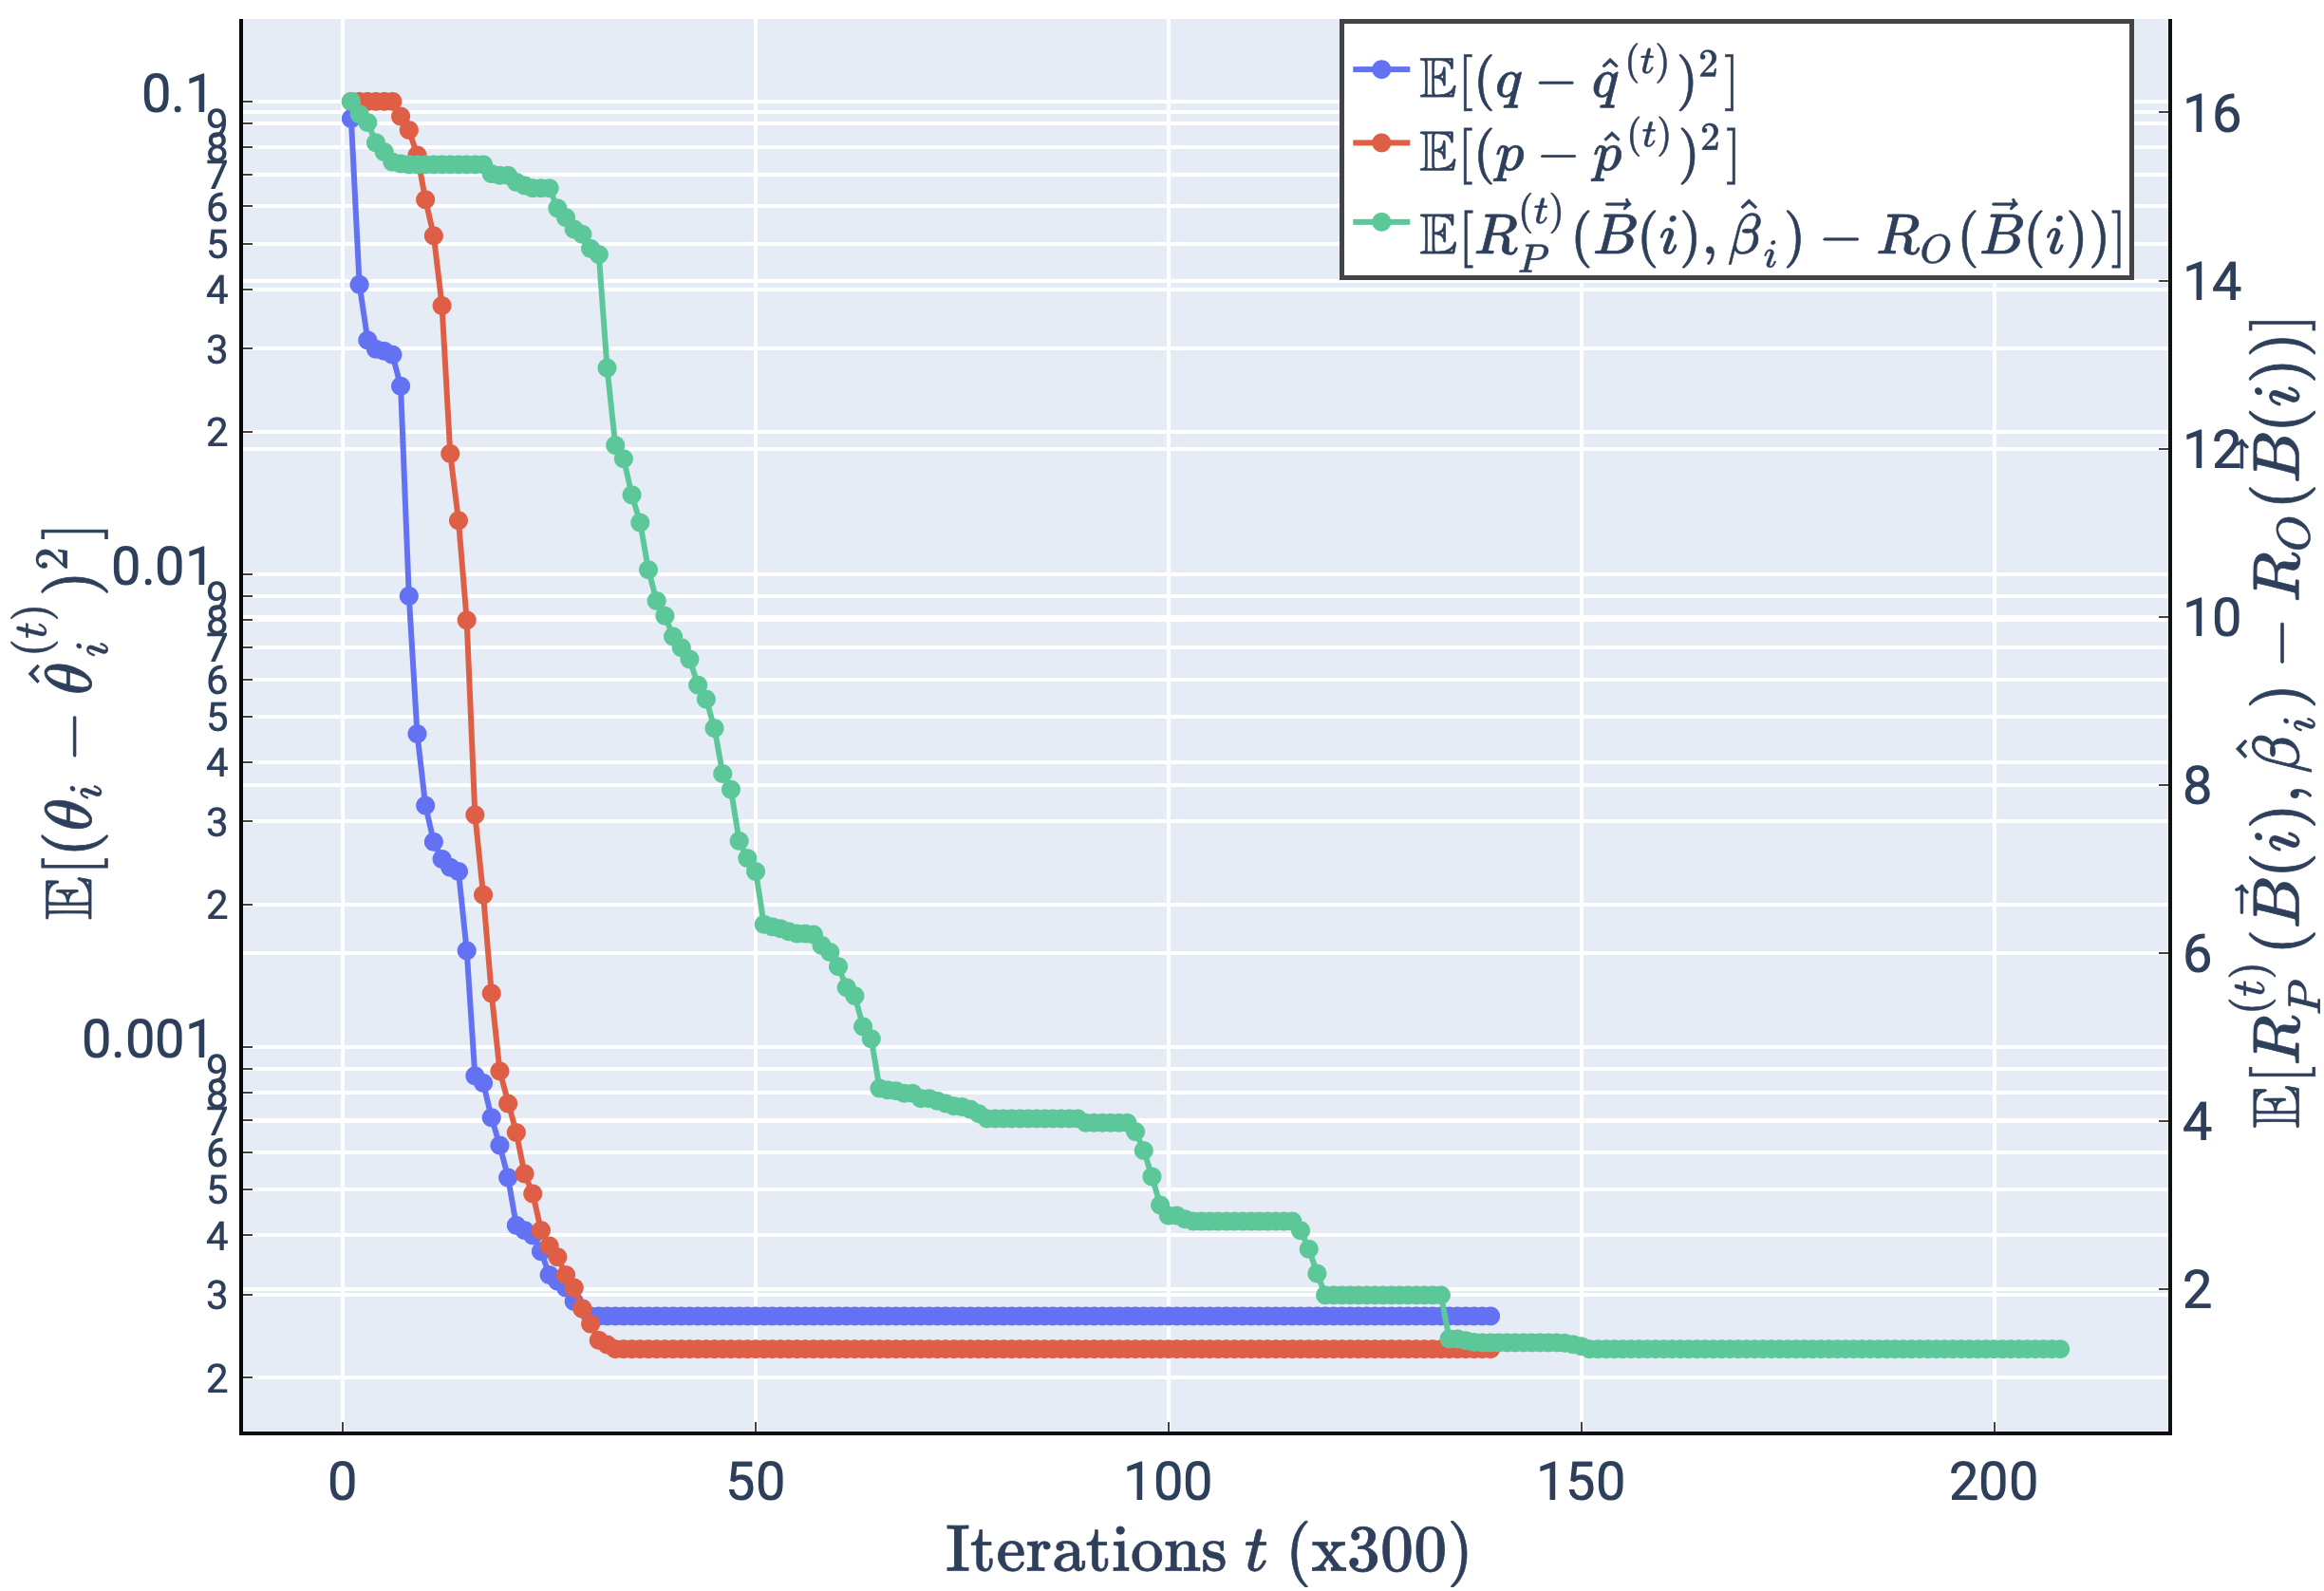
\includegraphics[width=0.80\linewidth]{PerseusRegretConvergence_MeanSquareErrorConvergence.png}
    \caption{Mean square error convergence of the parameter estimation algorithm while determining the correlation models $p$ and $q$, and the Regret convergence of the fragmented PERSEUS algorithm with belief simplification}
    \vspace{-5mm}
    \label{fig:4}
\end{figure}

Fig. \ref{fig:4} also illustrates the \emph{Regret} convergence plot of the PERSEUS algorithm, on the same time scale and in the same simulation run, over several iterations $t$, wherein the regret metric corresponds to the difference in utility obtained by our PERSEUS algorithm at a certain iteration $t$ in our simulation, denoted by $R_{P}^{(t)}(\vec{B}(i), \hat{\beta}_{i})$, and an \emph{Oracle} which has complete information about the occupancy behavior of incumbents in the network, whose utility is denoted by $R_{O}(\vec{B}(i))$. Starting with a random exploration phase to gather the set of reachable beliefs $\tilde{\mathcal{B}}$, the termination condition for the PERSEUS algorithm is that the number of policy changes, denoted by $\eta$, over several consecutive backup stages should be $0$. This trace in Fig. \ref{fig:4}, similar to the \emph{Reward v/s Time} plot in \cite{DBLP:journals/corr/abs-1109-2145}, serves as a measure of convergence for our fragmented PERSEUS algorithm with simplified belief updates and online model estimation.

We evaluate the performance of the proposed framework in terms of the SU network throughput and PU interference metrics over varying values of the penalty term $\lambda$ as illustrated in Fig. \ref{fig:8}. As surmised, we find that our POMDP agent decides to limit channel access when the penalty is high, leading to lower SU network throughput and lower PU interference; and on the other hand, it follows a more lenient channel access strategy when the penalty is low, resulting in higher SU network throughput and higher PU interference. In general, we observe the trend of rising throughput and increasing interference as the penalty for missed detections $\lambda$ is lowered. Comparing this performance of our proposed framework with correlation-coefficient based state-of-the-art, namely the MEM with MEI-CCE and MPE algorithm with $\rho_{th}{=}0.77$ and $6$ specified clusters, from \cite{6956794}, we find that our framework achieves higher SU network throughput and lower PU interference with $\lambda{\geq}10$. Furthermore, the proposed framework comes very close to achieving the throughput attained by a Viterbi agent \cite{4554696}, while providing the same interference performance. It is worth noting that the Viterbi agent possesses prior knowledge about the transition model of the underlying MDP and senses more channels per time-step than our POMDP agent. More importantly, the proposed framework allows us to regulate the trade-off between the interference caused to PUs and the throughput of the SU, by adjusting the parameter $\lambda$.
\vspace{-3.5mm}
\section{Conclusion}\label{V}
\begin{figure}
    \centering
    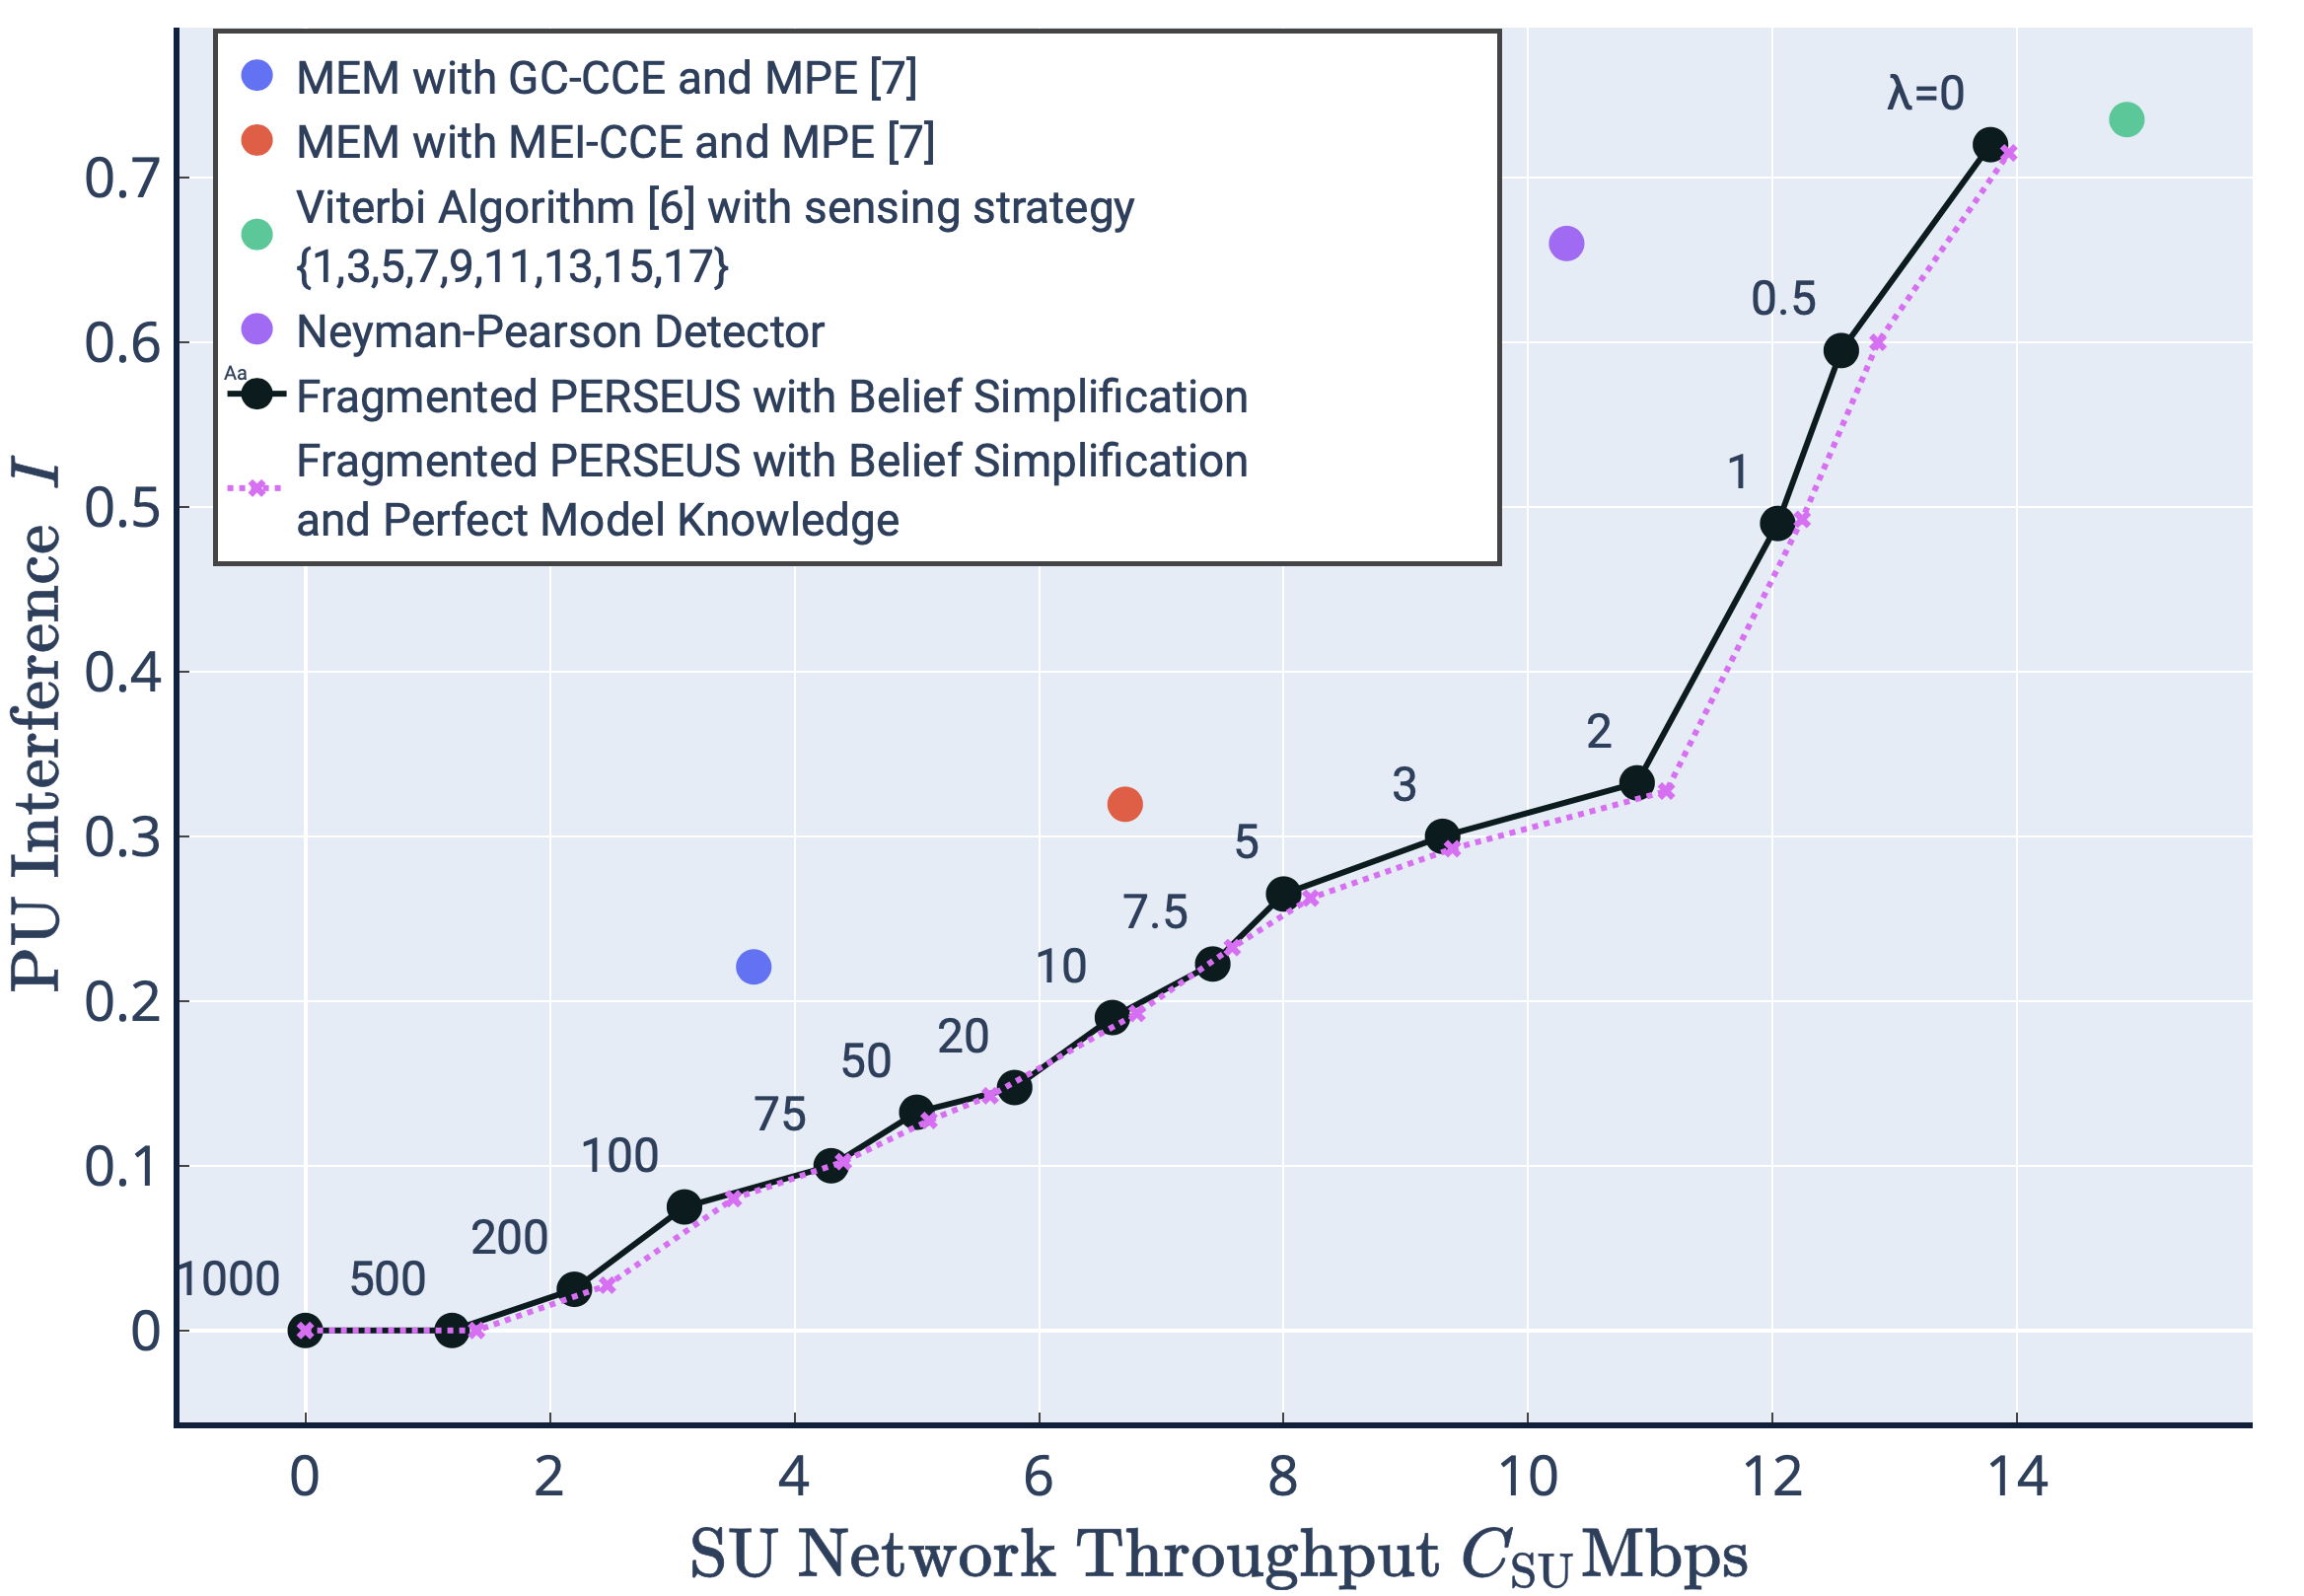
\includegraphics[width=0.80\linewidth]{SU_Throughput_PU_Interference_Varying_Penalty.png}
    \caption{SU Network Throughput versus PU Interference evaluation of the proposed framework over varying values of the penalty $\lambda$}
    \vspace{-5mm}
    \label{fig:8}
\end{figure}
In this paper, we formulate the optimal spectrum sensing and access problem in an AWGN observation model with multiple licensed users and a cognitive radio restricted in terms of its sensing capabilities, as a POMDP. In a radio environment wherein the occupancy behavior of the incumbents is correlated across time and frequencies, we present a consolidated framework that employs the EM algorithm to estimate the transition model of this occupancy behavior, and leverage a fragmented PERSEUS algorithm with belief update heuristics to simultaneously solve for the optimal spectrum sensing and access policy. Through system simulations, we conclude that our framework, in terms of the trade-off between secondary network throughput and interference to licensed users, out-performs the existing correlation-coefficient based clustering algorithms and a Neyman-Pearson detector that assumes independence among channels. Our framework is also capable of achieving the SU throughput and PU interference performance attained by a Viterbi algorithm that senses more channels per time-step, and that possess the correlation structure information \emph{apriori}.
\vspace{-5mm}

\bibliographystyle{IEEEtran}
\bibliography{ref}
\end{document}

\chapter{FEASIBILITY ANALYSIS OF THE POMDP OPTIMAL POLICY ON ESP$32$ RADIOS}\label{D}
In this chapter, we detail the implementation of the POMDP optimal spectrum sensing and access policy (from Chapter \ref{C}) on ad-hoc distributed network consisting of ESP32 radios, in order to prove the feasibility of our formulation. Section \ref{D.I} details the methodology followed in implementing the POMDP optimal sensing and access policy; Section \ref{D.II} describes the results obtained from this implementation; and Section \ref{D.III} involves concluding arguments.

\section{Methodology}\label{D.I}
We employ $8$ ESP32 radios \cite{Espressif:ESP32}, with each one embedded in a GCTronic e-puck2 robot \cite{GCTronic:epuck2}, categorized into a network of $3$ PUs (and their $3$ corresponding sinks) occupying $6$ channels in the discretized spectrum of interest according to a Markovian time-frequency correlation structure (described by \eqref{6})\texttt{-{}-}and $2$ independent SUs, with each having the capability of sensing only one channel at a time, intelligently trying to exploit the white-spaces in the spectrum. The detailed methodology of this implementation is provided below:
\begin{enumerate}
    \item Considering a network with $J{=}3$ PUs and one SU with a channel sensing restriction of $\kappa{=}2$ out of $K{=}6$ channels in the discretized spectrum of interest\texttt{-{}-}and assuming a linear AWGN observation model, with a Rayleigh channel fading model (discussed in Section \ref{I.I}), we simulate the occupancy behavior of the PUs according to a Markovian time-frequency correlation structure parameterized by $\vec{\theta}{=}[\vec{p},\vec{q}]^{\intercal}$, where $\vec{p}{=}[p_{00}{=}0.1,p_{01}{=}0.3,p_{10}{=}0.3,p_{11}{=}0.7]^{\intercal}$ and $\vec{q}{=}[q_{0}{=}0.3,q_{1}{=}0.8]^{\intercal}$; and solve for the optimal spectrum sensing and access policy using PERSEUS, embedded with a concurrent parameter estimation algorithm learning the parameter vector $\vec{\theta}$\texttt{-{}-}by mimicking the observational capabilities of the actual ESP32 radios. Note this step is performed on a PC.
    \item The simulated PU occupancy behavior\texttt{-{}-}Markovian correlated according to \eqref{6} and parameterized by $\vec{\theta}$, and the time-slot specific optimal channel access decisions (derived off of the POMDP optimal sensing policy and the simulated PU occupancy behavior), are stored in databases (for export onto the ESP32 network).
    \item Peer-to-Peer communication links are established between a PU ESP32 radio and its sink, using the $3$ ESP32 radios designated as PUs\texttt{-{}-}in other words, $3$ wireless communication links are established: one for each ESP32 PU pair (a source and a sink), over WiFi ($2.4$GHz) and using a channel according to the occupancy information detailed in the exported PU occupancy database, in time-slot $i$.
    \item Note here that in this ESP32 PU network implementation, in time-slot $i$, while establishing a wireless communication link between a ESP32 PU $j{\in}\{1,2,3\}$ and its respective sink $i{\in}\{1,2,3\}\text{ s.t.}i\text{ is the designated sink for PU}j$, i.e., while forming link $l_{ij}$ over channel $k_{l_{ij}}{=}k{\in}\{1,2,\dots,6\}$ (as determined by the exported PU occupancy database which contains simulated PU occupancy behavior according to the Markovian time-frequency correlation structure described above) such that $k_{l_{ij}}{\neq}k_{l_{i',j'}},{\forall}i,i'{\in}\{1,2,3\},j,j'{\in}\{1,2,3\}$\texttt{-{}-}PU $j$ serves as an Access Point (AP) accepting transmission requests from PU $i$, which is designates as a STAtion (STA). In the next synchronized time-slot $i+1$, this link $l_{ij}$ moves to channel $k'{\in}\{1,2,\dots,6\}$, as detailed in the exported PU occupancy database. This same procedure takes place for the other two incumbent communication links in every time-slot until the end of the implementation evaluation period.
    \item Although the PC-based POMDP solver employs an SU which can access $2$ channels at a time in order to deliver its flows (see the access part of the POMDP formulation in Section \ref{I.IV}), we employ $2$ ESP32 SU radios in the network\texttt{-{}-}with the channel access work synchronously and evenly split between the two\texttt{-{}-}due to the actual physical design limitation of the ESP32 radio that a it can only access one channel at a time, forcing us to be creative: split the optimal $2$ channel access decision in time-slot $i$, as determined by the time-slot specific optimal POMDP channel access database, into a single-channel access action at each ESP32 SU radio. Next, based on whether the channel access at the $2$ ESP32 SU radios was successful, we compute the success rate.
\end{enumerate}
\section{Implementation Results}\label{D.II}
The channel access success rate metric defined as
\begin{equation}\label{C.I}
    \text{Channel Access Success Probability}=\frac{\sum_{j=1}^{2}\mathcal{I}\left\{B_{k_{SU_{j}}}(i)=0\right\}}{2},
\end{equation}
where $\mathcal{I}$ corresponding to $\mathcal{I}\left\{B_{k_{SU_{j}}}(i)=0\right\}$ is an indicator variable whose value is $1$ if the channel accessed by the ESP32 SU $j{\in}\{1,2\}$ in time-slot $i$ is not occupied by an incumbent PU ESP32 radio, and $B_{k_{SU_{j}}}{\in}\{0,1\}$ is the occupancy variable of the channel accessed by the ESP32 SU $j$ in time-slot $i$\texttt{-{}-}is evaluated per time-slot $i$, and the resultant metrics are plotted against time, which is illustrated in Fig. \ref{fig:C.1}.
\begin{figure} [htb]
    \centerline{
    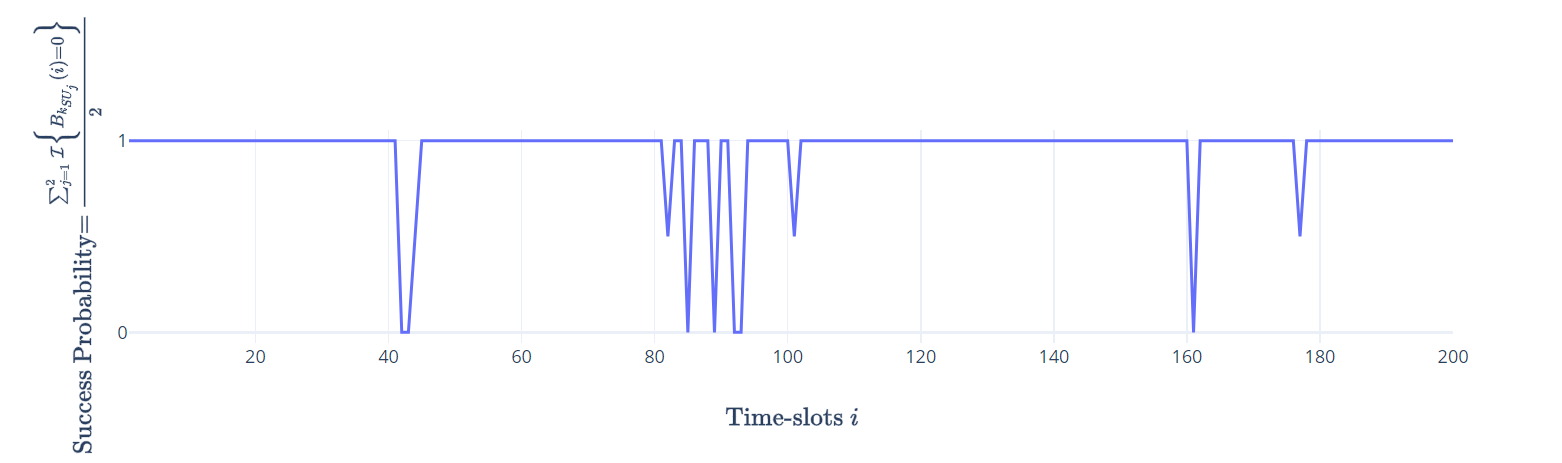
\includegraphics[width = 1.0\textwidth]{ESP32_Success_Probability.PNG}}
    \caption{The channel access probability of the ESP32 SU radios per time-slot}
    \label{fig:C.1}
\end{figure}
\section{Conclusion}\label{D.III}
In this chapter, we simulated an ad-hoc distributed peer-to-peer network with incumbent radios occupying the spectrum according to a Markovian time-frequency correlation structure, and an SU constituting a parameter estimator and a POMDP agent solving for the optimal channel sensing and access policy\texttt{-{}-}the simulated time-slotted incumbent occupancy behavior is exported onto a peer-to-peer network formed by actual ESP32 radios serving as PUs; and the time-slotted optimal channel access decisions are exported onto a peer-to-peer network formed by actual ESP32 radios serving as SUs (we use $2$ SUs in the actual implementation due to design limitations, with the access work split between the two, and merged upon completion). Upon merging the channel access results from both the ESP32 SU radios, we plot the SU network's success probability (given by \eqref{C.I})\texttt{-{}-}we find that the channel access decisions made by our SU network are accurate for a significant portion of the implementation evaluation period. The primary intention behind this analysis is to show that the optimal policy obtained by the POMDP solver with respect to an ad-hoc emulated network can be transferred (i.e., exported) onto the actual physical network with ease, by leveraging synchronization and data aggregation techniques.

%
%  summary.tex  2007-02-06  Mark Senn  http://www.ecn.purdue.edu/~mark
%

\chapter{SUMMARY}
Comprehending the need for spectrum sharing from an economic and national security point of view, in this work, we describe the various design principles involved in the development of cognitive radios, while specifically focusing on certain aspects of the design, proving their superiority to the state-of-the-art, and finally, their implementation feasibility. Detailing further, in this work, we describe the design principles underlying the operation of our cognitive radio in the DARPA SC2 Colosseum\texttt{-{}-}importantly, the CIRN architecture under which our networks were deployed in any given scenario, the OFDM PHY, the MCS adaptation algorithm driven by packet error rates, prioritized flow-scheduling involving a recursive-revisitation value-per-resource heuristic, the channel access algorithm driven by PSD measurements and collaboration messages, the CIL protocol, and multi-hop routing. Moreover, we present actual performance plots of these algorithms in DARPA SC2-emulated scenarios, in which the performance of our network is compared in real-time with that of other competitor networks deployed in the same scenario, in addition to an ensemble-view of the performance of all the networks in the scenario, to prove the need for collaboration among networks.

While acknowledging the possibility and potential of improvements in the other aspects of our radio's design, we focused our subsequent research particularly on the spectrum sensing and access algorithms in the MAC layer of the radio's network protocol stack and sought to improve it by adopting a rigorous mathematical approach as opposed to a more heuristic one incorporated in our DARPA SC2 radio. In this regard, in an AWGN observation model and a Raleigh fading channel model, we developed a POMDP formulation for channel sensing and access in a radio environment involving multiple incumbents exhibiting a time-frequency correlation structure in their occupancy behavior. In this POMDP formulation, in order to solve for the optimal channel sensing and access policy to be employed in the MAC layer of our radio, we designed an online parameter estimation algorithm leveraging tools from HMMs and MLE, and embedded it directly into a randomized point-based approximate value iteration method known as the PERSEUS algorithm with additional customizations such as fragmentation and belief update simplification. To prove the superiority of our POMDP framework for spectrum sensing and access, we have presented numerical evaluations of our algorithm against the state-of-the-art\texttt{-{}-}in doing so, we have proved that, for the same amount of deterioration in the throughput of the PUs in the network, our solution obtains a 37.5\% improvement in SU network throughput, compared to the MEM with MPE-MEI from \cite{WCL:7}; a 25\% improvement over a Neyman-Pearson Detector with no sensing restrictions from \cite{WCL:11}; and 6\% improvement over the Viterbi algorithm from \cite{WCL:6}. Critically, accounting for the need to handle deployment scenarios in which different interference constraints may be imposed at different times and in different geographical regions, our framework facilitates the trade-off between the SU network throughput and PU interference, by tuning the penalty parameter $\lambda$. Additionally, with this formulation, we drive home three crucial results: leveraging the time-frequency correlation structure exhibited in the occupancy behavior of the incumbents in the network leads to significant improvements in estimation accuracy, while allowing the radio to make wise decisions with limited information (due to channel sensing restrictions); adapting the spectrum sensing decisions according to past actions and their corresponding rewards leads to more white spaces being found for use by the cognitive radio; and an online EM algorithm for HMMs (known as the Baum-Welch algorithm) can be used to estimate the time-frequency occupancy correlation structure in tandem with a POMDP policy optimization algorithm, in non-stationary settings.

Finally, the performance metrics and illustrations presented from the POMDP optimal policy implementation experiment on an ad-hoc distributed network of ESP32 radios embedded on off-the-shelf e-puck2 robots, prove the simplicity in adapting the algorithms to different network setups and to different radio terminals having varying degrees of computational capabilities.

%
%  bibliography.tex     June 3, 2002     Mark Senn
%
%  This is the bibliography for a simple, example thesis.
%

\bibliography{all}

\end{document}
